%%% To fix widows and orphans, see:
%https://en.wikibooks.org/wiki/LaTeX/Page_Layout#Widows_and_orphans

%----------------------------------------------------------
%
\documentclass[letterpaper,12pt,openany,reqno]{book}%

%
%----------------------------------------------------------
% This is a sample document for the standard LaTeX Book Class
% Class options
%       --  Body text point size:
%                        10pt (default), 11pt, 12pt
%       --  Paper size:  letterpaper (8.5x11 inch, default)
%                        a4paper, a5paper, b5paper,
%                        legalpaper, executivepaperF
%       --  Orientation (portrait is the default):
%                        landscape
%       --  Printside:   oneside, twoside (default)
%       --  Quality:     final(default), draft
%       --  Title page:  titlepage, notitlepage
%       --  Columns:     onecolumn (default), twocolumn
%       --  Start chapter on left:
%                        openright(no, default), openany
%       --  Equation numbering (equation numbers on right is the default):
%                        leqno
%       --  Displayed equations (centered is the default):
%                        fleqn (flush left)
%       --  Open bibliography style (closed bibliography is the default):
%                        openbib
% For instance the command
%          \documentclass[a4paper,12pt,reqno]{book}
% ensures that the paper size is a4, fonts are typeset at the size 12p
% and the equation numbers are on the right side.
%
\usepackage{ulem}
\usepackage{amsmath}%
\usepackage{amsfonts}%
\usepackage{amssymb}%
\usepackage{graphicx}
\usepackage{subcaption}
\usepackage{tabulary}
\usepackage[colorlinks=true,linkcolor=blue]{hyperref}
%\hypersetup{pdfauthor={Philip Howard}, pdftitle={A Very Simple Compiler Book}}

\usepackage{tikz}
\usetikzlibrary{shapes,arrows.meta}


\usepackage{float}
\floatstyle{boxed} 
\restylefloat{figure}

\newfloat{mylisting}{thbp}{lob}[chapter]
\floatname{mylisting}{Listing}

\usepackage{listings}
\lstset{ %
xleftmargin={0.5in},						% left margin
language=C,                			% choose the language of the code
columns=flexible,
basicstyle=\small\ttfamily,     % the size of the fonts that are used for the code (was sffamily)
numbers=left,                   % where to put the line-numbers
numberstyle=\small,             % the size of the fonts that are used for the line-numbers
stepnumber=5,                   % the step between two line-numbers. If it's 1 each line will be numbered
numberfirstline=true,						% number the first line of the listing
firstnumber=1,									% auto or <number>
numbersep=5pt,                  % how far the line-numbers are from the code
%backgroundcolor=\color{white},  % choose the background color. You must add \usepackage{color}
showspaces=false,               % show spaces adding particular underscores
showstringspaces=false,         % underline spaces within strings
showtabs=false,                 % show tabs within strings adding particular underscores
frame=single,	                  % adds a frame around the code
tabsize=2,	                    % sets default tabsize to 2 spaces
captionpos=b,                   % sets the caption-position to bottom
breaklines=true,                % sets automatic line breaking
float=thbp,
%breakatwhitespace=false,        % sets if automatic breaks should only happen at whitespace
%title=\lstname,                 % show the filename of files included with \lstinputlisting; also try caption instead of title
%escapeinside={\%*}{*)}            % if you want to add a comment within your code
}


\lstnewenvironment{derivation}[2]
{
\lstset{float=htbp,caption={#1},label={#2},numbers=none}
\renewcommand{\lstlistingname}{Derivation}
}
{
\lstset{numbers=left}
\renewcommand{\lstlistingname}{Listing}
}

\lstnewenvironment{cfg}[2]
{
\lstset{float=htbp,caption={#1},label={#2},stepnumber=1,escapechar=Q}
\renewcommand{\lstlistingname}{CFG}
}
{
\lstset{numbers=left,stepnumber=5}
\renewcommand{\lstlistingname}{Listing}
}

\newcommand{\code}[1] {\lstinline[breaklines=yes,breakatwhitespace=yes]{#1}}

\newcommand{\cfgprod}[2] {{\ttfamily #1} $\rightarrow$ {\ttfamily #2}}
\newcommand{\cfgindentprod}[2] {\begin{quote} {\ttfamily #1} $\rightarrow$ {\ttfamily #2} \end{quote}}

%\usepackage[T1]{fontenc}  % access \textquotedbl
%\usepackage{textcomp}     % access \textquotesingle

\newcommand{\needswork}{\paragraph{This section needs work.}}
\newcommand{\needsproblems}{\paragraph{Add practice problems here.}}

%---------------------------------------------------
% commands for drawing FAs
\newcommand{\faterminalnode}[3] {\node at (#1) (#2) [circle, draw, double, minimum size=24pt] {#2};}
\newcommand{\fastart}[1] {\coordinate (start) at (#1);}
\newcommand{\fanonterminalnode}[2] {\node at (#1) (#2) [circle, draw, minimum size=24pt] {#2};}
\newcommand{\fanolabel}[2] {\node at (#1) (#2) [circle, draw, minimum size=24pt] {};}
\newcommand{\fatransition}[3] {\draw [->] (#1) -- (#2) node [midway, above] {#3};}
\newcommand{\fabelowtransition}[3] {\draw [->] (#1) -- (#2) node [midway, below] {#3};}
\newcommand{\farighttransition}[3] {\draw [->] (#1) -- (#2) node [midway, right] {#3};}
\newcommand{\faarctransition}[5] {\draw [->] (#1) to[out=#4, in=#5] node  [midway, above] {#3} (#2) ;}
\newcommand{\faarcbelowtransition}[5] {\draw [->] (#1) to[out=#4, in=#5] node  [midway, below] {#3} (#2) ;}
\newcommand{\faloopright}[2] {\draw (#1) edge [loop right] node {#2} ();}
\newcommand{\faloopleft}[2] {\path (#1) edge [loop left] node {#2} ();}
\newcommand{\falooptop}[2] {\path (#1) edge [loop above] node {#2} ();}
\newcommand{\faloopbottom}[2] {\path (#1) edge [loop below] node {#2} ();}
%---------------------------------------------------
% commands for drawing PDAs
\newcommand{\pdaterminal}[3] {\node at (#1) (#2) [rectangle, draw, rounded corners] {#3};}
\newcommand{\pdapush}[3] {\node at (#1) (#2) [rectangle, draw] {#3};}
\newcommand{\pdaread}[3] {\node at (#1) (#2) [diamond, draw] {#3}; }
\newcommand{\pdaconnect}[2] {\node at (#1) (#2) [circle, draw, minimum size=10pt] {};}
\newcommand{\pdatransition}[3] {\draw [->] (#1) -- (#2) node [midway, above] {#3};}
\newcommand{\pdaxthree}[4] {\draw [->] (#1) -- (#2) node [midway, above] {#4} -- (#3) ;}
\newcommand{\pdaxfour}[5] {\draw [->] (#1) -- (#2) node [midway, above] {#5} -- (#3) -- (#4);}
\newcommand{\pdarighttransition}[3] {\draw [->] (#1) -- (#2) node [midway, right] {#3};}
\newcommand{\pdalefttransition}[3] {\draw [->] (#1) -- (#2) node [midway, left] {#3};}

\newcommand{\pdaarctransition}[5] {\draw [->] (#1) to[out=#4, in=#5] node  [midway, above] {#3} (#2) ;}
\newcommand{\pdaloopright}[2] {\draw (#1) edge [loop right] node {#2} ();}

%---------------------------------------------------

\usepackage{mdwlist}
\newenvironment{mydesc}[1][9em]
  {
     \begin{basedescript}
     {
      \renewcommand{\makelabel}[1]{\bfseries##1}
      \desclabelwidth{ #1 }
      \desclabelstyle{\multilinelabel}
     }
  }
  {
     \end{basedescript}%
  }
\makecompactlist{mydesc*}{mydesc}

%----------------------------------------------------------
\newtheorem{theorem}{Theorem}
\newtheorem{acknowledgement}[theorem]{Acknowledgement}
\newtheorem{algorithm}[theorem]{Algorithm}
\newtheorem{axiom}[theorem]{Axiom}
\newtheorem{case}[theorem]{Case}
\newtheorem{claim}[theorem]{Claim}
\newtheorem{conclusion}[theorem]{Conclusion}
\newtheorem{condition}[theorem]{Condition}
\newtheorem{conjecture}[theorem]{Conjecture}
\newtheorem{corollary}[theorem]{Corollary}
\newtheorem{criterion}[theorem]{Criterion}
\newtheorem{definition}[theorem]{Definition}
\newtheorem{example}[theorem]{Example}
\newtheorem{exercise}[theorem]{Exercise}
\newtheorem{lemma}[theorem]{Lemma}
\newtheorem{notation}[theorem]{Notation}
\newtheorem{problem}[theorem]{Problem}
\newtheorem{proposition}[theorem]{Proposition}
\newtheorem{remark}[theorem]{Remark}
\newtheorem{solution}[theorem]{Solution}
\newtheorem{summary}[theorem]{Summary}
\newenvironment{proof}[1][Proof]{\textbf{#1.} }{\ \rule{0.5em}{0.5em}}
%----------------------------------------------------------


\begin{document}


%\tikz [foo /.tip = {Latex[length=3mm,width=2.5mm]} ]
%\tikz[arrows={[bend]}] 
\tikzset{ >=Latex }
\tikzset{arrows = {[length=3mm,width=2.5mm]} }

\frontmatter
\title{A Very Simple Grammars Book}
\author{Philip W. Howard}
\date{\today}
\maketitle
\tableofcontents
\listoffigures
\chapter{Preface}

I've been teaching Introduction to Grammars (aka Computer Theory) at Oregon Institute of Technology (OIT) for several years. OIT offers a very hands-on program, so why include a theory course? The most obvious answer is that it lays the theoretical background for a compiler class. I don't find that answer particularly compelling because to be successful in a compiler class a student needs a practical knowledge of some of the concepts included in a grammars class, but the student does not need the theoretical content to be successful in compilers.

To me, the primary reason for including the grammars class in our curriculum is precisely because it is a theory class. Requiring students to think abstractly, and to work on abstract problems (some of which are quite difficult) allows them to develop skills and thought processes that can be missed in a purely practical, hands-on program of study. These additional skills and thought processes will make them better equipped to solve some of the complex problems they may face in their professional careers.

So why did I decide to write a text for this class? There is a Computer Theory text that I really like, but it has become criminally expensive (as I'm writing this, Amazon would be glad to sell you a new paperback edition for over \$500). I could not, in clear conscience, ask my students to purchase a book at that price. I found an Open text that could be legally downloaded free; a print-on-demand paperback version could be purchased for under \$10. It was a good text, but it was ``too mathematical'' for my purposes. I want my students to be able to wrestle with concepts without getting bogged down with too much notation. So I decided to attempt my own.

I hope that this book proves useful to my students, and if it is discovered by others, that it is useful to them as well.

Phil Howard
\mainmatter
%%%%%%%%%%%%%%%%%%%%%%%%%%%%%%%%%%%%%%%%%%%%%%%%%%%%
%% FORMATTING
\setlength{\parindent}{0cm} % Default is 15pt.
\setlength{\parskip}{8pt plus 2pt minus 2pt}
%%%%%%%%%%%%%%%%%%%%%%%%%%%%%%%%%%%%%%%%%%%%%%%%%%%%

\part{Introduction}
My grammars students often wonder why we include a theory course in an otherwise very hands-on program. My answer, ``Because grammars is fun!'' doesn't seem to carry much weight, so I offer the following list of benefits to studying this topic:

\begin{enumerate}
\item The grammars course lays the theoretical foundation for the compilers course. What does a compiler do? It implements several formal language processors. What is a formal language? That's part of what is learned in the grammars course.
\item You will be better at what you're being trained to do if you can think abstractly. A theory course helps you do that.
\item Many programming problems can be made much easier if you can transform the problem to a different domain. The grammars class illustrates ways this is done. If you ``get'' the mechanism, you can apply it elsewhere.
\item As you are stretched, you grow. By facing difficult challenges in your course work, you are better equipped to face difficult challenges in your professional work.
\item And besides, grammars is fun!
\end{enumerate}

\chapter{Introduction}
\section{Historical Background}
\needswork
\section{Formal Languages}
Computer theory deals with what is known as ``formal languages''. They aren't formal in the sense that you use them when talking to important people (as opposed to the informality that you allow when shooting the breeze with friends). They are formal in the sense that they conform to a specific (usually mathematical) form. In particular, given a statement, it is always possible to answer the question, ``Is that statement a valid statement in this formal language?'' English does not meet this definition. Consider all the red ink used by English teachers while grading freshmen compositions. The writers thought their statements were valid English, the but teachers disagreed.

Figure~\ref{F.formal.language.processor} illustrates what a formal language processor does. Any arbitrary input can be fed into the processor, and it answers the question, ``Is the input a valid statement in the language?''. It always returns ``yes'' or ``no''. If the language is a formal language, there can be no ``maybe''.

%----------------------------------------------------------
\begin{figure}[hbt]
\centering
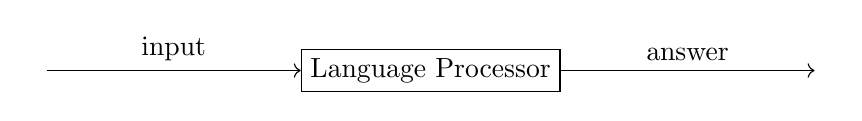
\begin{tikzpicture}
\node (a) at (-5,0) {};
\node (b) at (0,0) [shape=rectangle, draw] {Language Processor};
\node (c) at (5,0) {};

\draw [->] (a) -- (b) node [midway, above] {input} ;
\draw [->] (b) -- (c) node [midway, above] {answer} ;
%\draw [->] (b) -- (c) node [midway, above, text width=3cm, align=center] {improved\\code} ;
\end{tikzpicture}
 \caption[Formal language processor]{A formal language process is fed some input and it returns one of two answers: The input is a valid statement in the language or The input is not a valid statement in the language.}
  \label{F.formal.language.processor}
\end{figure}
%----------------------------------------------------------

If you attempted to create a Language Processor for English, it should probably reject statements like, ``Cup sky red Perl''. Rejecting that statement might be easy enough, but could you create a processor that accepts all valid English (including English poetry), and rejects all non-English. To get a sense of the difficulty of this challenge, I refer you to poetry by ee cummings (capitalization is correct). The poetry of ee cummings is considered valid (and even good) English poetry by those who get to decide such things, but it would likely be rejected my any sensible English language validity checker.

Those who study formal languages usually restrict themselves to very simple languages. As an example, consider the language of all strings consisting of any combination of the letters ``a'' and ``b''. This language includes strings such as ``aaaa'' and ``abababbbb''. It isn't useful for anything outside the study of formal languages, but it is an example of a formal language.

The study of formal languages is tightly coupled with mathematical sets. In particular, a formal language is a set of strings. Specifically, the set of all strings that meet the definition of the language.  This book assumes you are familiar with mathematical sets including the operations union, intersection, and subtraction. If you aren't familiar with these operations, I'm sure there's a Wikipedia page that can help you out.

Formal languages consist of the following:
\begin{enumerate}
\item An alphabet: a set of characters that the strings in the language are composed of. The alphabet for a language is often represented by the symbol $\Sigma$.
\item A definition of what strings are in the language.
\end{enumerate}

Let's illustrate with an example. 

\begin{quote}
$\Sigma = \{ a \ b \}$

All strings of five letters.
\end{quote}

Given this definition, the string ``aaxbb'' would be rejected because 'x' is not in the alphabet. The string ``aabb'' would likewise be rejected because it consists of four letters, not five. However, the strings, ``aaaaa'', ``aabbb'', and ``ababa'' would all be included in the language (along with many others).

Formal languages can be broken into categories based on the mechanism used to specify the language. We will initially be interested in three types of definitions, which are discussed in the following chapters.
\begin{enumerate}
\item Recursive definitions (not to be confused with Recursive Languages discussed in Part~\ref{C.Beyond.Context.Free} of the book)
\item Regular Expressions
\item Context Free Grammars
\end{enumerate}

\chapter{Recursive Definitions}
Recursion is a useful technique in writing some computer programs. It is also a useful technique in specifying formal languages. Consider the following two definitions of the set EVEN:
\begin{enumerate}
\item The set of all positive integers divisible by 2
\item A recursive definition:
\begin{enumerate}
\item 2 is in EVEN
\item If $x$ is in EVEN then $x+2$ is in EVEN.
\end{enumerate}
\end{enumerate}

Which of these two definitions is the most useful? Probably the first one. If you wanted to prove the 96 is in EVEN using the first definition, a simple division by 2 suffices. If you wanted to prove this using the second definition, it would take a bit longer. But there are other instances where a recursive definition is quite elegant.

Consider the following non-recursive definition of arithmetic expressions:
\begin{enumerate}
\item $\Sigma = \{ number\ +\ -\ *\ /\ (\ ) \}$
\item Can't have two operators in a row
\item Must have balanced parenthesis
\item Can't have two numbers in a row
\item Can't begin or end with an operator
\end{enumerate}

Is this set of rules sufficient? Do they allow every valid arithmetic expression? Do they preclude every invalid expression? Could you argue from these rules that the following is (or isn't) a valid arithmetic expression?
\begin{quote}
$(2+7)/3-(((4+5)*(6)-1)*3 + 4)$
\end{quote}
How about:
\begin{quote}
$()()(2+7)/3-(((4+5)*(6)-1)*3 + 4)$
\end{quote}
This last expression meets the definition given above, but is not a valid arithmetic expression because of the empty parenthesis. We could add a rule that states you can't have empty parenthesis, which would rule out the expression above. How about the expression:
\begin{quote}
$)))4((($
\end{quote}
This expression has balanced parenthesis (the same number of opens as closes), but they happen to be in the wrong order. We could fix that by specifying that parenthesis have to be properly nested. Then what about the expression:
\begin{quote}
$5(*)7$
\end{quote}
As you can see, there seems to be a never ending combination of ways to thwart our set of rules, so how can we know when we have a complete set? When we can't think of any new ways to break our set? What if someone more creative (or evil) comes along and finds a way to break the rules that we hadn't thought of.

Let's try a recursive definition for arithmetic expressions (called AE in the definition):

\begin{enumerate}
\item Any number is in AE
\item If $f$ and $g$ are in AE, then so are:
\begin{enumerate}
\item $f + g$
\item $f - g$
\item $f * g$
\item $f / g$
\item $(f)$
\end{enumerate}
\end{enumerate}
I claim (without proof) that this is a complete set of rules that always works.

How can we use this definition to prove an expression is a valid arithmetic expression? We do so by construction: invoke the various rules one at a time until the desired expression is constructed. Let's do so with the expression:
\begin{quote}
$(2+7)/5$
\end{quote}
The construction is as follows:
\begin{enumerate}
\item $2$ is in AE (Rule 1)
\item $7$ is in AE (Rule 1)
\item $2+7$ is in AE (Points 1 and 2 and Rule 2b)
\item $(2+7)$ is in AE (Point 3 and Rule 2e)
\item $5$ is in AE (Rule 1)
\item $(2+7)/5$ is in AE (Points 4 and 5 and Rule 2d)
\end{enumerate}
Having constructed the desired expression using the rules, we have proven that it is a valid arithmetic expression. (More formally, we have proven that it is in the language AE as defined above).

How do we prove that an expression is not in AE? This is a bit more complicated. Take the expression given above:
\begin{quote}
$()()(2+7)/3-(((4+5)*(6)-1)*3 + 4)$
\end{quote}
Let's generalize it to the statement:
\begin{quote}
Valid statements in AE never have empty parenthesis.
\end{quote}

Before proving this statement, we will prove a different one:
\begin{quote}
Valid statements in AE never start with a close parenthesis and never end with an open parenthesis.
\end{quote}
The proof is as follows:
\begin{enumerate}
\item Numbers do not contain parenthesis, so Rule~1 cannot create an AE that starts with a close parenthesis or ends with an open parenthesis.
\item If $f$ and $g$ do not start with a close parenthesis or end with an open parenthesis, none of the Rule 2's will create a string that starts with a close parenthesis or ends with an open parenthesis.
\item Since there is no way to construct a string that starts with a close parenthesis or ends with an open parenthesis, such a string does not exist in AE.
\end{enumerate}

Back to empty parenthesis: We could prove this using a similar mechanism to what we just used. However, we will use proof by contradiction just to illustrate this mechanism. With this style of proof, you assume the opposite of what you want to prove and then reason until you encounter a contradiction. Since you got to a contradiction, your assumption must have been false. Note: as we will see later, it is important that you only make a single assumption. The contradiction means at least one of your assumptions was false. If you've made multiple assumptions, you don't know which one is false.

Let's assume that a string in AE can contain empty parenthesis. Let's define $s$ as the shortest string that contains empty parenthesis. The string $s$ must be constructed using one of the rules. Which one? Let's consider them one at a time:
\begin{enumerate}
\item Numbers do not contain parenthesis, so $s$ cannot be constructed using Rule~1.
\item The empty string is not a valid number. Rules 2a-2e add characters to the string, and no rules subtract characters from the string. Therefore, it is not possible to have an empty string in AE.
\item Rules 2a-2d do not add parenthesis to the string so they cannot create $s$.
\item Rule 2e will create an empty set of parenthesis if either:
\begin{enumerate}
\item $f$ is the empty string 
\item $f$ begins with a close parenthesis or ends with an open parenthesis
\end{enumerate}
However, we've already proven that neither of these can happen.
\item Since there is no way to construct $s$, our assumption must be false and we can conclude that a string in AE cannot contain empty parenthesis.
\end{enumerate}

\section{Constructing Recursive Definitions}
We've seen several recursive definitions. What do they have in common? A recursive definition is always composed of two parts:
\begin{itemize}
\item Base Cases that identify some set of strings in the language. The base case for AE was ``Any number is in AE''.
\item Recursive Rules of the form, ``If $x$ is in L, then so is $f(x)$''. Rules 2a-2e for AE are the recursive rules. Recursive rules can use multiple variables as illustrated in the definition of AE.
\end{itemize}

When constructing recursive definitions, it is important to keep in mind what the language is. For example, the language AE was a set of strings. As a result, rules 2a-2e were adding characters to the string, they were not performing arithmetic operations. The language EVEN was a set of numbers, so Rule~b was performing an arithmetic operation to create a new number.

If the language is a set of strings, then the recursive rules always extend or combine strings. That is, they always make longer strings, they never remove characters from the string. In other words, you should never have a rule of the form, ``If $x$ is in L, then so is $x$ without the trailing semicolon.''

As another example of a recursive definition, consider the following definition of Polynomial:
\begin{enumerate}
\item Any number is in Polynomial
\item The variable $x$ is in Polynomial
\item If $f$ and $g$ are in Polynomial, then so are:
\begin{enumerate}
\item $f+g$
\item $f-g$
\item $f g$
\item $f/g$
\item $(f)$
\end{enumerate}
\end{enumerate}

Note 1: In Rule~3c, $f g$ is used to represent the multiplication of $f$ and $g$. Polynomials are mathematical expressions, so we are using the mathematical notation for multiplication. If we were using a programming language notation, this rule would probably read $f*g$.

Note 2: like AE, this is a set of strings so the arithmetic operators in Rule~3 are simply characters, no arithmetic operations are performed. 

Given this definition, it should be easy enough to show that $(24/4/2)$ is in Polynomial (note that it is also in AE). What is the meaning of this expression? is it $3$ or $12$ (based on which operation is performed first). It turns out this is an erroneous question. Both Polynomial and AE are sets of strings. We can answer the question, ``Is this string in the language?'', but the question ``What does this string mean?'' is not relevant to these languages.

In programming languages, there is syntax and semantics. One way of thinking of these two is that syntax deals with the question, ``Is this a valid statement in the formal language?'' Semantics deals with the question, ``What is the meaning of this statement?'' or even, ``Does this statement have a valid meaning in the language?''. At this point, we are only concerned with syntax, not semantics.

\section{Summary}
Recursive definitions provide a mechanism to construct formal languages. A recursive definition consists of base cases and recursive rules that are used to extend the language. The mechanism we presented here isn't very mathematically rigorous, so we can't prove many properties about the languages that are generated by these definitions (a short-coming that won't be found in the next several chapters). One thing we can say about languages generated by recursive definitions is that they are always infinite. That is, they always contain an infinite number of words. This is true because there is no limit on how many times a recursive rule can be invoked, and each invocation produces a new word in the language.

\section{Problems}
\begin{enumerate}
\item Given the definition of Polynomial given in this chapter argue either that the statement $x^3 + 4x^2 -7$ either is or is not in Polynomial.
\item The definition of Polynomial given in this chapter only allows a single variable. Extend the definition to allow two variables.
\item The language PALINDROME is the set of all strings that read the same forwards and backwards. Give a recursive definition of even-length PALINDROMEs over $\Sigma = \{a\ b\}$. 
\item Extend your definition of PALINDROME to include both even and odd length strings.
\item Give a recursive definition of positive integers (or argue that it can't be done).
\item Give a recursive definition of positive rational numbers (or argue that it can't be done).
\item Give a recursive definition of positive real numbers (or argue that it can't be done).
\item Give a recursive definition for the set of strings over $\Sigma=\{0 1 2 3 4 5 6 7 8 9\}$ that cannot start with the digit zero.
\end{enumerate}

\part{Regular Languages}
\chapter{Regular Expressions}
Many programmers are familiar with regular expressions from non-compiler contexts. Examples include using an asterisk (*) as a wildcard in a file name, or specifying patterns for the \code{grep} utility. Different programs use different syntax for specifying regular expressions. In this chapter a minimalist syntax for all regular expressions is presented. Most programs that interpret regular expressions enhance this syntax in various ways to make writing regular expressions easier, but the added syntax does not add extra capabilities. In this chapter, we are not interested in programs that make use of regular expressions, so we don't need the syntactic sugar that many of them add. Instead, we are interested in the formal languages that can be specified using regular expressions.

Regular expressions include the following features:
\begin{mydesc}[10em]
	\item[Concatenation] Concatenation is gluing two strings end-to-end. For example, concatenating ``\code{ab}'' with ``\code{bc}'' yields the string ``\code{abcd}''.
  \item[Alternation] Alternation means to choose exactly one from a set of alternatives. Regular expressions use either the vertical bar (\code{|}) or the plus sign (\code{+}) to mean alternation. So the expression \code{a + b + c} means to choose either an '\code{a}', a '\code{b}', or a '\code{c}'. 
	\item[Grouping] Parenthesis can be used for grouping operations much as they can in algebraic expressions.
	\item[Kleene Closure] Kleene Closure means to take zero or more instances of a string. Kleene Closure is denoted by an asterisk ($^*$). So, for example, $x^*$ means zero or more '$x$' characters. Kleene Closure has higher precedence than concatenation so that $ab^*$ means $a(b^*)$ not $(ab)^*$.
\end{mydesc}

In addition to these operations, the $\Lambda$ symbol is used to represent an empty string (a string with no characters in it).

The most common enhancements to this syntax are as follows:
\begin{mydesc}
\item[zero or one] The question mark
 (\code{?}) 
indicates zero or one of an item so that \code{a?} 
means the same as ($\Lambda$ \code{+ a}).
\item[one or more] The plus sign (\code{+}) is similar to Kleene Closure, but it is one-or-more not zero-or-more so that \code{a+} means the same as $aa^*$.
\item[character range] Square brackets (\code{[]}) can be used to specify a character range so that \code{[a-m]} means any single character in the range '\code{a}' through '\code{m}'. This could be represented long-hand as '\code{(a + b + c + d + ...)}'.
\end{mydesc}

These enhancements will be used in a few examples, and they are allowed in homework problems provided their use is clear. Note that the one-or-more enhancement uses the plus sign that can also be used for concatenation so any regular expression that uses \textbf{any} of these enhancements must use the vertical bar for alternation.

If we want a regular expression for integer constants, we could try
\begin{quote}\code{[0-9]+}\end{quote}
but this allows any number of leading zeros. A better expression would be:
\begin{quote}\code{[1-9][0-9]*}\end{quote}
This fixes the leading zero problem, but it does not allow the number zero. This can be fixed as follows:
\begin{quote}\code{0 | ([1-9][0-9]*)}\end{quote}
If we want to allow negative numbers, we could add an optional minus sign:
\begin{quote}\code{0 | (-?[1-9][0-9]*)}\end{quote}

There are exercises at the end of the chapter that can be used to practice writing regular expressions. You use the enhanced syntax or the minimal syntax for these exercises.

\section{Manipulating Regular Expressions}

Regular expressions look similar to algebraic expressions, so it might be tempting to manipulate them as if they were algebraic expressions. Some manipulations are possible, but the rules can be quite different from algebra. For example, in both regular expressions and algebra,
\begin{quote}
$a(b+c) = ab + ac$
\end{quote}
but the following have no algebraic equivalent:
\begin{quote}
$(a^*)^* = a^*$\\
$(a+b^*)^* = (a+b)*$\\
$(a^*b^*)^* = (a+b)^*$
\end{quote}

\section{Language Families}
Each regular expression defines a language.\footnote{These languages are not unique; it is possible to write multiple regular expressions for the same language.} Remember that a formal language is a set of strings. Also recall that it is possible to have a set of sets, so what can we say about the set of all languages that can be defined by regular expressions? This set is known as Regular Languages. They are ``regular'' in the sense that they can be defined by a regular expression. Regular languages have a set of properties that they share. We will eventually explore what these properties are. 

We can also think of the set of all regular expressions. This is yet another language (set of strings). We can give a recursive definition of this language, but we cannot give a regular expression for it because, as we shall see, it is not regular.

\begin{enumerate}
\item Every letter in $\Sigma$ is in RE
\item If $r_1$ and $r_2$ are in RE, then so are:
\begin{enumerate}
\item $r_1 r_2$
\item $r_1 + r_2$
\item $r_1^*$
\item $(r_1)$
\end{enumerate}
\end{enumerate}

So we now have three separate but related languages:
\begin{itemize}
\item The language (set of all strings) defined by a particular regular expression.
\item The set of all languages definable by regular expressions.
\item The set of all regular expressions.
\end{itemize}

It is important to keep these three languages separate. Consider the following questions, one for each category of language:
\begin{itemize}
\item What is the language defined by $(a + b)^*a(a + b)^*$? This question is asking you to enumerate (or otherwise describe) a particular regular language.
\item Is the language L regular? This is asking whether the specific language L is in the set of all languages definable by regular expressions.
\item Is the statement, $a + (b + c)+$ a regular expression? This is asking ``Is it a well-formed regular expression?'' or ``Is it in the language for regular expressions that we gave a recursive definition for?''
\end{itemize}

In the coming sections we want to examine properties of regular languages (properties of the entire family of regular languages, not of a particular regular language). We will do a couple of them now.

First of all, how do you prove a language is regular? The obvious solution is to write a regular expression that generates the language. One needs to be careful to make sure the regular language actually generates the correct language. For example, if one asked, ``Is the language L of all strings over $\Sigma = \{a\ b\}$ which contain at least one $a$ and at least one $b$ regular?''
The regular expression
\begin{quote}
$(a+b)^*a(a+b)^*b(a+b)^*$
\end{quote}
would not be proof that it was. All strings generated by this regular expression contain at least one \code{a} and at least one \code{b}. However, the string \code{ba} is part of L, but it cannot be generated by the specified regular expression. In other words:
\begin{quote}
$(a+b)^*a(a+b)^*b(a+b)^* \subset L$
\end{quote}

This is not sufficient proof that L is regular. It is always possible to give a regular subset of any language. This can be done by giving a alternation of a finite list of words from the language. The ability to show there is a regular subset of the language is not sufficient proof that the language is regular.

A regular expression that generates a language is adequate proof that the language is regular (provided the regular expression actually corresponds to the language). How can we prove a language isn't regular? An inability to write a regular expression for the language is not sufficient proof. The statement, ``I can't write a regular expression for that language'' might be because the language isn't regular or it might be because you simply aren't creative (or smart or persistent) enough to come up with one. Chapter~\ref{C.RL.theory} provides a mechanism to prove a language isn't regular. 

Theorem~\ref{TH.finite.languages} gives the first property we will prove regarding regular languages.
\begin{theorem}
\label{TH.finite.languages}
All finite languages are regular.
\end{theorem}

The proof is quite simple. If a language is finite, every word in the language can be enumerated. The list might be very long, but it can be generated. A regular expression that corresponds to this language is simply the alternation of each word in the language:
\begin{quote}
(word\_1) + (word\_2) + \dots + (word\_n)
\end{quote}

Before proving other properties of regular languages, we have a question to answer.

\section{Why Regular Languages?}
We've identified a class of languages known as ``Regular Languages'' --- namely, those languages that can be defined by regular expressions. Why is this class of languages interesting? From a theory point of view, they are interesting because they form the smallest class of languages in what's known as the Chompsky Hierarchy of languages. Later parts of the text will deal with the larger classes of languages in the hierarchy, all of which are supersets of regular languages. 

From a practical point of view, regular languages are useful because they are fast and efficient to process. By ``process'', we mean answering the question, ``Is this input a member of a particular regular language?'' A common application of this is the \code{grep} utility included with most Linux distributions. With \code{grep}, you specify a regular expression and an input file, and \code{grep} identifies all lines of the file that include a match for the regular expression\footnote{This is a simplification of what \code{grep} does, but it is accurate for the purposes of this illustration}. Most uses of regular expressions include ``scanning'' for a match. A text string (often the contents of a text file) is read looking for a match to the regular expression. How efficient are regular expressions scanners? Theorem~\ref{TH.O.N.for.res}, which won't be proven until later, gives a bound on their efficiency.
\begin{theorem}
\label{TH.O.N.for.res}
Any regular expression can be scanned for in $O(N)$ with small time constant where $N$ is the length of the input string.
\end{theorem}

The next chapter discusses a ``machine'' that can perform this processing.

\section{Exercises}
\begin{enumerate}
\item Write a regular expression for a string containing any odd number of the letter \code{a}.
\item Write a regular expression for C (or Java) variable names. Valid characters include upper and lower case letters, digits, and the underscore (\code{\_}).
\item Write a regular expression for a string containing a positive even number of \code{a}'s followed by an odd number of \code{b}'s. The following are valid strings: \code{aaaabbb}, \code{aabaabaabbb}, \code{aaaaaabbbbbaabaabaab}. The following are not valid strings: \code{aaab}, \code{aaaabbbaa}, \code{bbbaab}.
\item For the previous question, state why each of the non-valid strings are not valid.
\item Write a regular expression for a floating-point constant. The following rules apply: 
\begin{enumerate}
\item The integer part cannot have leading zeros unless the integer part is zero. 
\item If there is a decimal point, it must be followed by at least one digit.
\item The decimal part must not have trailing zeros unless the decimal part is zero.
\end{enumerate}
For the following problems, give an English definition of the language defined by the specified regular expressions. Don't simply transliterate the regular expressions. For example, for the regular expression $a^*b(a+b)^*$, you should not say, ``Any number of $a$'s followed by a $b$ followed by any combination of characters.'' Instead, you should say ``All strings with a $b$.

Assume $\Sigma = \{a\ b\}$ unless otherwise specified.

\item $(a+b)^*a(a+b)^*b(a+b)^*$
\item $(aa + ab + ba + bb)^*$
\item $(a+b)(aa + ab + ba + bb)^*$
\item $((a+b)(a+b))^*$
\end{enumerate}

\chapter{Finite Automata}
There is a well-known children's game called Chutes and Ladders. The goal is to be the first player to move their piece from the beginning (bottom) to the ending (top) of the board. On a player's turn, they spin a spinner which lands on a number. The player advances their piece the specified number of squares on the board. If their piece lands on the bottom of a ladder, they climb the ladder thus making extra progress towards their goal. If their piece lands on the top of a chute, they slide down the chute winding up closer to the beginning. This game is considered a ``children's'' game because it involves no strategy. The outcome of the game is completely determined by the sequence of numbers generate by the spinner (assuming the players don't cheat).

What does this game have to do with regular expressions or finite automata? If we assume that the spinner only generates numbers less than ten (single digit numbers), then we could spin the spinner a bunch of times and write down each result. The result would be a string of digits. We could then ask the question, ``Does this sequence of moves result in someone winning the game?'' That still doesn't sound like a regular expression question (although scanning a string sounds familiar), so let's think of a Finite Automaton\footnote{``Automaton is the singular of the plural ``Automata''.} (aka state machine).

A finite automaton consists of a finite number of states (or configurations) and transitions from state to state. How could we turn Chutes and Ladders into a state machine? Suppose there were three players. Each player's marker could be on any of the squares on the board. Each configuration of markers (each player on each valid square in every combination) could be considered a state. There would be a large number of states, but the number would be finite. Transitions consist of moves such as ``Player~2 moves forward three spaces''. Each state would have an outbound transition for each possible spinner result for each player. The finite automaton representation of the game makes it clear that there is no strategy involved. The machine process the input (the sequence of spins) without any human involvement. The outcome is determined solely by the sequence of spins. But the question still remains, ``What does this have to do with regular expressions?''

Before we answer that question (through some other examples), lets define a standardized way of graphically representing finite automata. Finite automata consist of a finite number of states and transitions between states. One state is defined as the start state, and any number of states can be defined as final states. The start state in an FA is signified by an inbound arrow that doesn't originate from another state. Processing always starts in the start state. Final states are signified by a double circle. Transitions are labeled by the letter that is used to move from one state to another. This format is illustrated in Figure~\ref{F.FA_1}.

%----------------------------------------------------------
\begin{figure}[hbt]
\centering
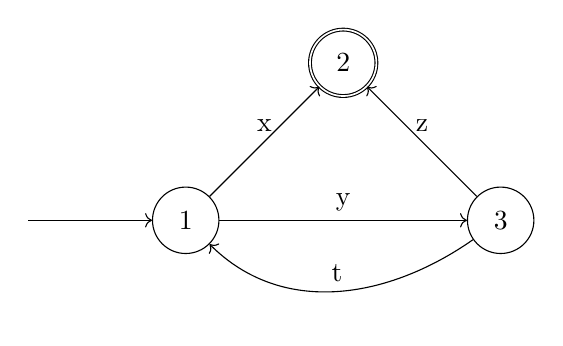
\begin{tikzpicture}

\fastart {-4, -2};
\fanonterminalnode {-2,-2}{1};
\faterminalnode {0,0}{2};
\fanonterminalnode {2,-2}{3};

\fatransition{start}{1}{};
\fatransition{1}{2}{x};
\fatransition{1}{3}{y};
\fatransition{3}{2}{z};
\faarctransition {3}{1}{t}{215}{315};

\end{tikzpicture}
 \caption[Sample Finite Automaton]{This is a sample FA. State~1 is the start state (it has an incoming arrow from nowhere). State~2 is a final state (signified by the double-circle). The transitions are labeled by what letter is used to move from one state to another.}
  \label{F.FA_1}
\end{figure}
%----------------------------------------------------------

Using the FA in Figure~\ref{F.FA_1}, and the input $ytx$, the processing starts in State~1 (the start state). The $y$ is used to transition to State~3. The $t$ is used to transition back to State~1. The $x$ is used to transition to State~2. Since the input is exhausted while in a final state, the string is accepted by the FA.

Two conditions can cause a string to be rejected: 
\begin{enumerate}
\item If the input is exhausted and the current state isn't a final state. The input $yty$ illustrates this case.
\item If there is no outbound transition on the current letter. The input $yx$ illustrates this case.
\end{enumerate}

Given these rules for processing FA's, it can be shown that the FA in Figure~\ref{F.FA_1} is equivalent to the regular expression $(yt)^* (x + yz)$. It is no coincidence that there is a regular expression that corresponds to the FA. It turns out that every FA is equivalent to some regular expression, and that each regular expression has an FA that is equivalent to it. We will prove this in a later section.

Figure~\ref{F.FA_2} gives another FA. This FA shows a slightly different format. The start state has a '-' in the label. Final states have a '$+$' in them. The states can be thought of as follows:
\begin{enumerate}
\item State 1: the start state.
\item State 2: An $a$ not preceded by an $a$.
\item State 3: A $b$ not preceded by a $b$.
\item State 4: Have read a double letter.
\end{enumerate}
Note that once a double letter has been found, the FA remains in the final state no matter what other letters are read.

%----------------------------------------------------------
\begin{figure}[hbt]
\centering
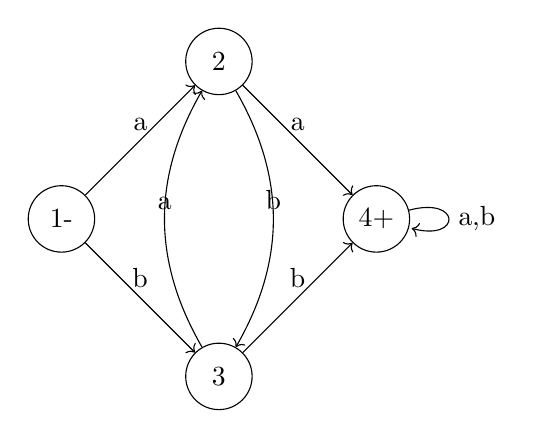
\begin{tikzpicture}

\fanonterminalnode {-2,0}{1-};
\fanonterminalnode {2,0}{4+};
\fanonterminalnode {0,2}{2};
\fanonterminalnode {0,-2}{3};

\fatransition{1-}{2}{a};
\fatransition{1-}{3}{b};
\fatransition{2}{4+}{a};
\fatransition{3}{4+}{b};
\faarctransition{3}{2}{a}{120}{240};
\faarctransition {2}{3}{b}{300}{60};
\faloopright {4+}{a,b};
\end{tikzpicture}
 \caption[FA for double letters]{This FA accepts all strings that contain a double letter.}
  \label{F.FA_2}
\end{figure}
%----------------------------------------------------------

FA's can also be represented in table form. These tables are called transition tables. The transition table for the FA in Figure~\ref{F.FA_2} is given in Figure~\ref{T.FA.2}. There is one row for each state. The state name is given in the first column. The remaining columns indicate the new state based on the transition letter at the top of the column.

%----------------------------------------------------------
\begin{figure}[hbt]
\centering
\begin{tabular}{|c|c|c|}
\hline
Current State & a & b \\
\hline
1- & 2 & 3 \\
\hline
2 & 4 & 3 \\
\hline
3 & 2 & 4 \\
\hline
4+ & 4 & 4 \\
\hline
\end{tabular}
\caption[Transition Table]{This transition table represents the same FA as Figure~\ref{F.FA_2}}
\label{T.FA.2}
\end{figure}

\section{Non-deterministic Finite Automata}

The FA illustrated in Figure~\ref{F.FA_1} is a Deterministic Finite Automaton (DFA). It is deterministic in the sense that for each character that is processed, the FA has exactly one choice on what to do. There is another class of FA's known as Non-deterministic Finite Automata (NFA's). With NFA's, for a given input, there is the potential for multiple choices on what to do. The choices can take two forms:
\begin{enumerate}
\item Multiple outbound edges labeled with the same letter. If that letter is read, any of the outbound edges labeled with that letter can be taken. This is illustrated by the edges from Node~$a$ labeled $z$ in Figure~\ref{F.NFA_1}.
\item Edges labeled $\Lambda$. These edges can be taken without consuming an input character. Node~$a$ has a $\Lambda$ transition meaning you can leave Node~$a$ without consuming any characters.
\end{enumerate}

%----------------------------------------------------------
\begin{figure}[hbt]
\centering
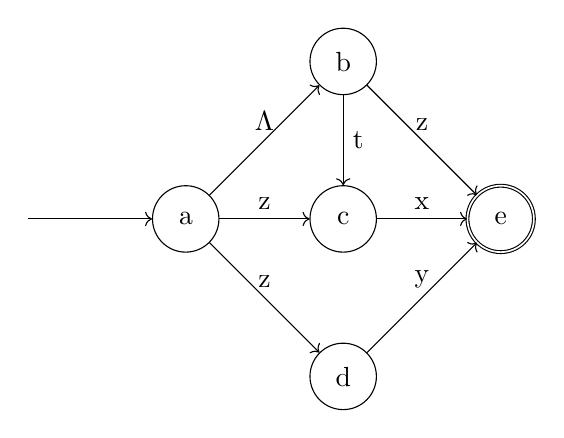
\begin{tikzpicture}

\fastart {-4, 0};
\fanonterminalnode {-2,0}{a};
\fanonterminalnode {0,2} {b};
\fanonterminalnode {0,0} {c};
\fanonterminalnode {0,-2} {d};
\faterminalnode {2,0} {e};

\fatransition{start}{a}{};
\fatransition{a}{b}{$\Lambda$};
\fatransition{a}{c}{z};
\fatransition{a}{d}{z};
\fatransition{b}{e}{z};
\farighttransition{b}{c}{t};
\fatransition{c}{e}{x};
\fatransition{d}{e}{y};

\end{tikzpicture}
 \caption[Sample Non-deterministic Finite Automaton]{This is a sample NFA. Node $a$ has multiple outbound transitions on $z$. It also has an outbound transition on $\Lambda$ meaning you could leave Node~$a$ without consuming any characters.}
  \label{F.NFA_1}
\end{figure}
%----------------------------------------------------------

The NFA in Figure~\ref{F.NFA_1} accepts the following stings:
\begin{mydesc}[2em]
	\item[$z$] This string is accepted by following the $\Lambda$ transition to Node~$b$ and then using the $z$ to transition to Node~$e$.
	\item[$tx$] This string is accepted by following the $\Lambda$ transition to Node~$b$ and then using the $t$ to transition to Node~$c$ and the $x$ to transition to Node~$e$.
	\item[$zx$] This string is accepted by using the $z$ to transition to Node~$c$ and then using the $x$ to transition to Node~$e$.
	\item[$zy$] This string is accepted by using the $z$ to transition to Node~$d$ and then using the $y$ to transition to Node~$e$.
\end{mydesc}

NFA's aren't any more powerful than DFA's--anything you can do with an NFA you can also do with a DFA\footnote{Section~\ref{S.Subset.Construction} gives a construction that can turn any NFA into an equivalent DFA. This is sufficient to argue that anything that can be done with an NFA can also be done with a DFA.}. The reason for introducing NFA's is that converting from a regular expression to code that accepts strings matching that regular expression makes use of NFA's.

\section{Thompson's}

The first step in converting a regular expression to executable code is to convert it to an equivalent NFA. For this conversion, we are going to use Thompson's Construction\footnote{Credited to Ken Thompson, the originator of the Unix operating system.}. The beauty of Thompson's construction is that it is a mechanical process -- one that doesn't require any creative thought. In other words, it can be automated. A computer program can be written to perform this conversion.

If two FA's each have a single start state and a single final state, and if the start state doesn't have any inbound edges and the final state doesn't have any outbound edges, then the two FA's can be composed by connecting the end state of one FA to the start state of the other using a $\Lambda$ transition. Thompson's Construction makes use of this fact by showing how to compose FA's for each operation supported by regular expressions (concatenation, alternation, and Kleene Closure). An NFA can be built for any regular expression simply by composing it one small piece at a time using Thompson's three diagrams. Figure~\ref{F.Thompsons} shows the three base diagrams.


%----------------------------------------------------------
\begin{figure}[htb]
\centering

%\scalebox{.7}{
\begin{subfigure}[b]{0.45\textwidth}
\centering
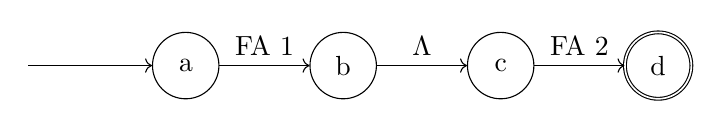
\begin{tikzpicture}
\fastart {0, 0};
\fanonterminalnode {2,0} {a};
\fanonterminalnode {4,0} {b};
\fanonterminalnode {6,0} {c};
\faterminalnode {8,0} {d};

\fatransition{start}{a}{};
\fatransition{a}{b}{FA 1};
\fatransition{b}{c}{$\Lambda$};
\fatransition{c}{d}{FA 2};

%\node at (5,-1) {Concatenation};
%\node at (5,-2) {};
\end{tikzpicture}
\caption{Concatenation}\label{F.Thompsons.Concatenation}
\end{subfigure}
%}

%\scalebox{.7}{
\begin{subfigure}[b]{0.45\textwidth}
\centering
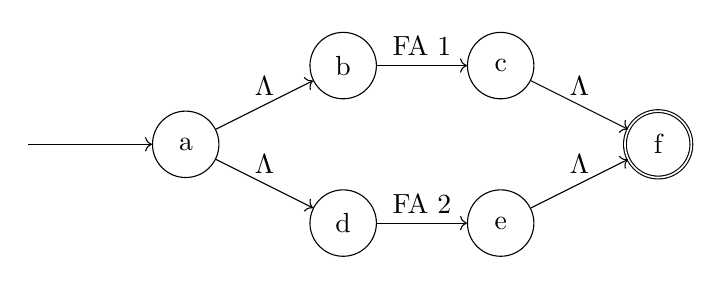
\begin{tikzpicture}
\fastart {0, 0};
\fanonterminalnode {2,0} {a};
\fanonterminalnode {4,1} {b};
\fanonterminalnode {6,1} {c};
\fanonterminalnode {4,-1} {d};
\fanonterminalnode {6,-1} {e};
\faterminalnode {8,0} {f};

\fatransition{start}{a}{};
\fatransition{a}{b}{$\Lambda$};
\fatransition{b}{c}{FA 1};
\fatransition{c}{f}{$\Lambda$};

\fatransition{a}{d}{$\Lambda$};
\fatransition{d}{e}{FA 2};
\fatransition{e}{f}{$\Lambda$};
%\node at (5,-2) {Alternation};
%\node at (5,-3) {};
\end{tikzpicture}
%}
\caption{Alternation}\label{F.Thompsons.Alternation}
\end{subfigure}

%\scalebox{.7}{
\begin{subfigure}[b]{0.45\textwidth}
\centering
%Kleene Closure
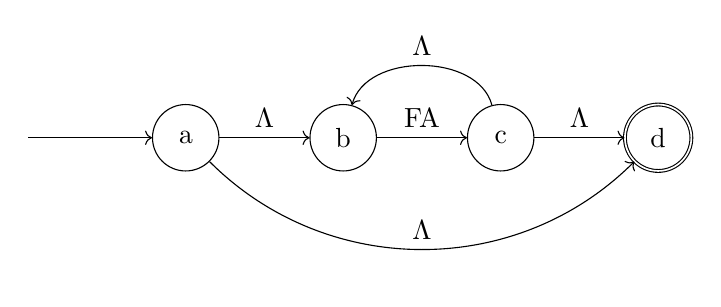
\begin{tikzpicture}
\fastart {0, 0};
\fanonterminalnode {2,0} {a};
\fanonterminalnode {4,0} {b};
\fanonterminalnode {6,0} {c};
\faterminalnode {8,0} {d};

\fatransition{start}{a}{};
\fatransition{a}{b}{$\Lambda$};
\fatransition{b}{c}{FA};
\fatransition{c}{d}{$\Lambda$};
\faarctransition {a}{d}{$\Lambda$}{315}{225};
\faarctransition {c}{b}{$\Lambda$}{105}{75};

%\node at (5,-2) {Kleene Closure};
%\node at (5,-3) {};
\end{tikzpicture}
%}
\caption{Kleene Closure}\label{F.Thompsons.KleeneClosure}
\end{subfigure}

 \caption[Thompson's Construction]{Thompson's Construction method makes use of these three diagrams. For each diagram, the FA(s) being composed are represented as two nodes (the start and end nodes) labeled $FA$, $FA 1$, or $FA 2$.}
  \label{F.Thompsons}
\end{figure}
%----------------------------------------------------------

The trick to using Thompson's construction is to NOT be creative. Each FA built with Thompson's has a single start and a single final state. The diagram can be dropped as-is directly into the next step in the construction. Nodes never need to be erased, and each composition should be drawn exactly as shown in Figure~\ref{F.Thompsons}.

Let's illustrate by doing several constructions. First, let's construct an NFA for \code{a (b + c)}. It's best to start with the inner most operation (in this case \code{(b + c)}) and work out. So first draw the alternation diagram as shown below:

\begin{center}
\scalebox{.7}{
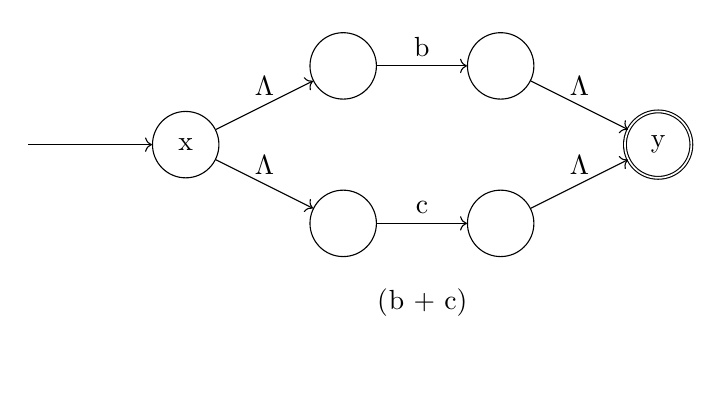
\begin{tikzpicture}
\fastart {0, 0};
\fanonterminalnode {2,0} {x};
\fanolabel {4,1} {b1};
\fanolabel {6,1} {b2};
\fanolabel {4,-1} {c1};
\fanolabel {6,-1} {c2};
\faterminalnode {8,0} {y};

\fatransition{start}{x}{};
\fatransition{x}{b1}{$\Lambda$};
\fatransition{b1}{b2}{b};
\fatransition{b2}{y}{$\Lambda$};

\fatransition{x}{c1}{$\Lambda$};
\fatransition{c1}{c2}{c};
\fatransition{c2}{y}{$\Lambda$};

\node at (5,-2) {\code{(b + c)}};
\node at (5,-3) {};
\end{tikzpicture}
} % end scaled box
\end{center}
The resulting diagram gets dropped into the \code{FA 2} position of the concatenation diagram as illustrated below. Note how the node labeled $x$ in the above diagram is in the location of the node labeled $c$ in the concatenation diagram, and the $y$ node is in the $d$ position.

\begin{center}
\scalebox{.7}{
\begin{tikzpicture}
\fastart {0, 0};
\fanonterminalnode {2,0} {s};
\fanolabel {4,0} {a1};

\fanonterminalnode {6,0} {x};
\fanolabel {8,1} {b1};
\fanolabel {10,1} {b2};
\fanolabel {8,-1} {c1};
\fanolabel {10,-1} {c2};
\faterminalnode {12,0} {y};

\fatransition{start}{s}{};
\fatransition{s}{a1}{a};
\fatransition{a1}{x}{$\Lambda$};


\fatransition{x}{b1}{$\Lambda$};
\fatransition{b1}{b2}{b};
\fatransition{b2}{y}{$\Lambda$};

\fatransition{x}{c1}{$\Lambda$};
\fatransition{c1}{c2}{c};
\fatransition{c2}{y}{$\Lambda$};

\node at (7,-2) {\code{a (b + c)}};
\node at (7,-3) {};
\end{tikzpicture}
} % end scalebox
\end{center}

As a second example, let's construct an NFA for $a (b + c)^*$. This is the same as the previous example, except that the alternation is wrapped in Kleene Closure. The alternation is, again, the innermost operation, and it is the same as in the previous example:

\begin{center}
\scalebox{.7}{
\begin{tikzpicture}
\fastart {0, 0};
\fanonterminalnode {2,0} {x};
\fanolabel {4,1} {b1};
\fanolabel {6,1} {b2};
\fanolabel {4,-1} {c1};
\fanolabel {6,-1} {c2};
\faterminalnode {8,0} {y};

\fatransition{start}{x}{};
\fatransition{x}{b1}{$\Lambda$};
\fatransition{b1}{b2}{b};
\fatransition{b2}{y}{$\Lambda$};

\fatransition{a}{c1}{$\Lambda$};
\fatransition{c1}{c2}{c};
\fatransition{c2}{y}{$\Lambda$};

\node at (5,-2) {\code{(b + c)}};
%\node at (5,-3) {};
\end{tikzpicture}
} % end scaled box
\end{center}

This is now dropped into the Kleene Closure construction:

\begin{center}
\scalebox{.7}{
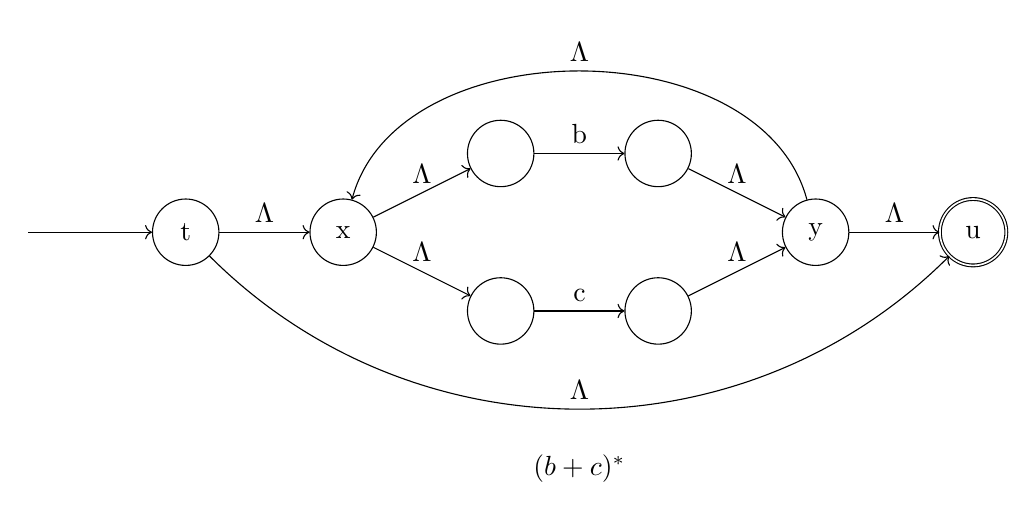
\begin{tikzpicture}
\fastart {0, 0};
\fanonterminalnode {2,0} {t}
\fanonterminalnode {4,0} {x};
\fanolabel {6,1} {b1};
\fanolabel {8,1} {b2};
\fanolabel {6,-1} {c1};
\fanolabel {8,-1} {c2};
\fanonterminalnode {10,0} {y};
\faterminalnode {12,0} {u};

\fatransition{start}{t}{};
\fatransition{t}{x}{$\Lambda$};
\fatransition{x}{b1}{$\Lambda$};
\fatransition{b1}{b2}{b};
\fatransition{b2}{y}{$\Lambda$};

\fatransition{x}{c1}{$\Lambda$};
\fatransition{c1}{c2}{c};
\fatransition{c2}{y}{$\Lambda$};

\fatransition{y}{u}{$\Lambda$};

\faarctransition {t}{u}{$\Lambda$}{315}{225};
\faarctransition {y}{x}{$\Lambda$}{105}{75};

\node at (7,-3) {$(b + c)^*$};
\end{tikzpicture}
} % end scaled box
\end{center}

Finally, we drop this into the concatenation construction:
\begin{center}
\scalebox{.7}{
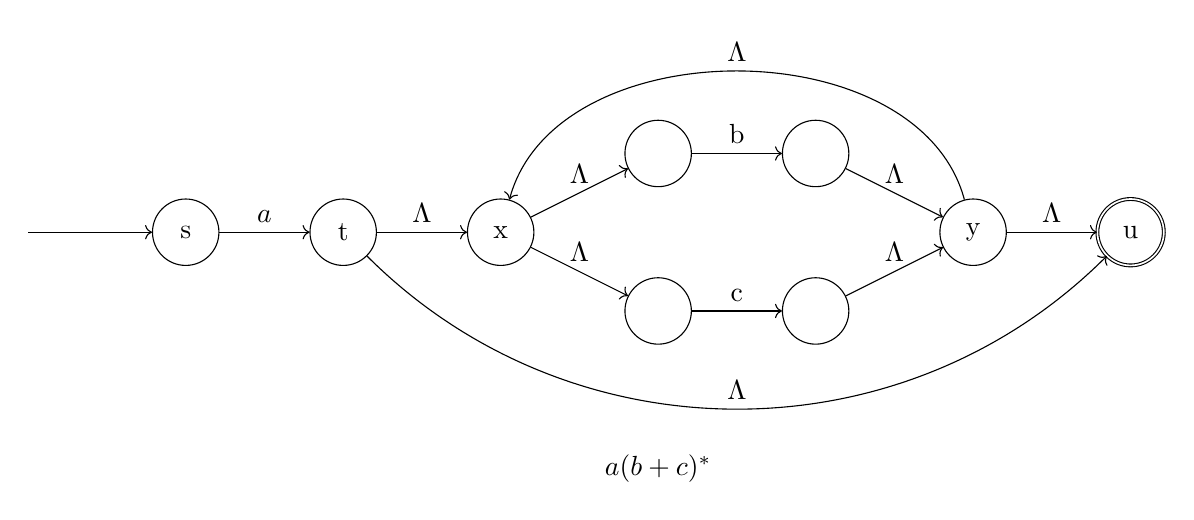
\begin{tikzpicture}
\fastart {0, 0};
\fanonterminalnode {2,0} {s}
\fanonterminalnode {4,0} {t}
\fanonterminalnode {6,0} {x};
\fanolabel {8,1} {b1};
\fanolabel {10,1} {b2};
\fanolabel {8,-1} {c1};
\fanolabel {10,-1} {c2};
\fanonterminalnode {12,0} {y};
\faterminalnode {14,0} {u};

\fatransition{start}{s}{};
\fatransition{s}{t}{$a$};
\fatransition{t}{x}{$\Lambda$};
\fatransition{x}{b1}{$\Lambda$};
\fatransition{b1}{b2}{b};
\fatransition{b2}{y}{$\Lambda$};

\fatransition{x}{c1}{$\Lambda$};
\fatransition{c1}{c2}{c};
\fatransition{c2}{y}{$\Lambda$};

\fatransition{y}{u}{$\Lambda$};

\faarctransition {t}{u}{$\Lambda$}{315}{225};
\faarctransition {y}{x}{$\Lambda$}{105}{75};

\node at (8,-3) {$a (b + c)^*$};
\end{tikzpicture}
} % end scaled box
\end{center}

As a third example, $a^* (b + c)$, includes a concatenation of two complex items
$a^*$ and $(b + c)$ ). To construct this, 
first construct $a^*$, 
then construct $(b + c)$ and then use the concatenation construction to combine them. Here is the resulting diagram:

\begin{center}
\scalebox{.7}{
\begin{tikzpicture}
\fastart {0, 0};
\fanonterminalnode {2,0} {t};
\fanolabel {4,0} {b};
\fanolabel {6,0} {c};
\fanonterminalnode {8,0} {u};

\fatransition{start}{t}{};
\fatransition{t}{b}{$\Lambda$};
\fatransition{b}{c}{a};
\fatransition{c}{u}{$\Lambda$};
\faarctransition {a}{u}{$\Lambda$}{315}{225};
\faarctransition {c}{b}{$\Lambda$}{105}{75};

\fanonterminalnode {10,0} {x};
\fanolabel {12,1} {b1};
\fanolabel {14,1} {b2};
\fanolabel {12,-1} {c1};
\fanolabel {14,-1} {c2};
\faterminalnode {16,0} {y};

\fatransition{u}{x}{$\Lambda$};
\fatransition{x}{b1}{$\Lambda$};
\fatransition{b1}{b2}{b};
\fatransition{b2}{y}{$\Lambda$};

\fatransition{x}{c1}{$\Lambda$};
\fatransition{c1}{c2}{c};
\fatransition{c2}{y}{$\Lambda$};

\node at (8,-2) {$a^* (b + c)$};
\node at (5,-3) {};
\end{tikzpicture}
} % end scaled box
\end{center}

It should be clear that Thompson's construction creates lots of $\Lambda$ transitions. This begs the question, ``isn't there an simpler way to draw these?''. The answer is in two parts. If by ``simpler'' you mean ``easier construction'', my answer would be ``no''. The whole point of Thompson's construction is that it is a simple mechanical process. It requires no creative thought. But if by ``simpler'' you mean a less complex result (one without all the $\Lambda$s), then the answer is ``yes''. The next section gives an algorithm to convert these complex NFAs into DFAs (diagrams without any $\Lambda$ transitions. The goal is not to make the diagram simpler, the goal is to get a DFA because they are easier to process in code.

\section{Subset Construction}\label{S.Subset.Construction}

To illustrate how an NFA could be processed, let's consider again the NFA for $a^* (b + c)$ presented in the last section, but presented again in Figure~\ref{F.subsetNFA}. In this figure, each node is labeled so they can be explicitly referred to. For each state, we can ask the question, ``What states could I wind up in if I encounter a particular letter in the input?''. For example, suppose we haven't consumed any input yet, what states could we be in? Clearly we could be in State~$1$, the start state, but because of the $\Lambda$ transitions, we could also be in states $2, 4, 5, 6, 8$. This set of states ($=\{1, 2, 4, 5, 6, 8\}$)\footnote{When specifying sets of characters,  it is often easier to read the list of items if each item is separated with a comma. This works unless the set included a comma (as sets of characters for a compiler often do). I will generally included commas for readability unless the set of characters includes punctuation (commas or other punctuation marks). I hope this will improve readability.}
forms a meta-state (let's call it $A$). From the meta-state~$A$, where could we wind up if we read an $a$. Since the meta-state~$A$ includes state~$2$, we can follow the $a$ to state~$3$. From there we can follow $\Lambda$s to $2, 4, 5, 6, 8$. This gives another meta-state. Let's call it $B = \{2, 3, 4, 5, 6, 8\}$. 

\begin{figure}[hbt]
\centering
\scalebox{.7}{
\begin{tikzpicture}
\fastart {0, 0};
\fanonterminalnode {2,0} {1};
\fanonterminalnode {4,0} {2};
\fanonterminalnode {6,0} {3};
\fanonterminalnode {8,0} {4};

\fatransition{start}{1}{};
\fatransition{1}{2}{$\Lambda$};
\fatransition{2}{3}{a};
\fatransition{3}{4}{$\Lambda$};
\faarctransition {a}{4}{$\Lambda$}{315}{225};
\faarctransition {3}{2}{$\Lambda$}{105}{75};

\fanonterminalnode {10,0} {5};
\fanonterminalnode {12,1} {6};
\fanonterminalnode {14,1} {7};
\fanonterminalnode {12,-1} {8};
\fanonterminalnode {14,-1} {9};
\faterminalnode {16,0} {10};

\fatransition{4}{5}{$\Lambda$};
\fatransition{5}{6}{$\Lambda$};
\fatransition{6}{7}{b};
\fatransition{7}{10}{$\Lambda$};

\fatransition{5}{8}{$\Lambda$};
\fatransition{8}{9}{c};
\fatransition{9}{10}{$\Lambda$};

\end{tikzpicture}
} % end scaled box
\caption[NFA produced by Thompson's]{This is the NFA produced by Thompson's for the regular expression $a^* (b + c)$}
  \label{F.subsetNFA}
\end{figure}

We could continue to find new meta-states by enumerating all possible outbound inputs from each meta-state and then following the $\Lambda$s from the resulting states. The results are presented in Table~\ref{T.subsetTable1}.

\begin{table}[hbt]
\center
\begin{tabular}{l|l|l|l}
\hline
\textbf{meta-state} & \textbf{NFA states} & \textbf{input} & \textbf{resulting states} \\
\hline
A & 1, 2, 4, 5, 6, 8 & a & 2, 4, 5, 6, 8 \\
A & 1, 2, 4, 5, 6, 8 & b & 7, 10 \\
A & 1, 2, 4, 5, 6, 8 & c & 9, 10 \\
B & 2, 4, 5, 6, 8 & a & 2, 4, 5, 6, 8 \\
B & 2, 4, 5, 6, 8 & b & 7, 10 \\
B & 2, 4, 5, 6, 8 & c & 9, 10 \\
C & 7, 10 & a & - \\
C & 7, 10 & b & - \\
C & 7, 10 & c & - \\
D & 9, 10 & a & - \\
D & 9, 10 & b & - \\
D & 9, 10 & c & - \\
\hline
\end{tabular}
\caption[Result of subset construction]{The results of performing the subset construction on the NFA in Figure~\ref{F.subsetNFA}. An input of ``-'' means there are no valid inputs starting from this state. Resulting states of ``-'' mean there are no valid destinations from this state.}
\label{T.subsetTable1}
\end{table}

We need a formal algorithm for producing these tables. The steps are as follows:
\begin{enumerate}
\item From the start state, follow all $\Lambda$s. Follow as many as you can, not just one. This is known as the $\Lambda$ closure of a state: all states reachable from a given state following only $\Lambda$s. This set of states is labeled $A$ in the table.
\item Make multiple rows, one for each character in the source-language, for each meta-state not already in the table. Initially this is only meta-state~$A$, and for the example NFA in Figure~\ref{F.subsetNFA}, the characters in the source language are $a, b, c$ meaning three rows for each meta-state.
\item For each NFA state in the meta-state, if there is an outbound transition on the input, write down the destination state in the resulting states column.
\item Extend the list of states in the resulting states column by forming the $\Lambda$ closure of each state already in the column.
\item If there are any new unique sets of states in the resulting states column, give them a unique label and return to Step~2.
\end{enumerate}
The process will stop once all existing rows are filled in and no new rows get generated.

Let's use these rules to derive a table for the NFA below. Note: this NFA was \textbf{not} generated with Thompson's.

\begin{center}
\scalebox{.7}{
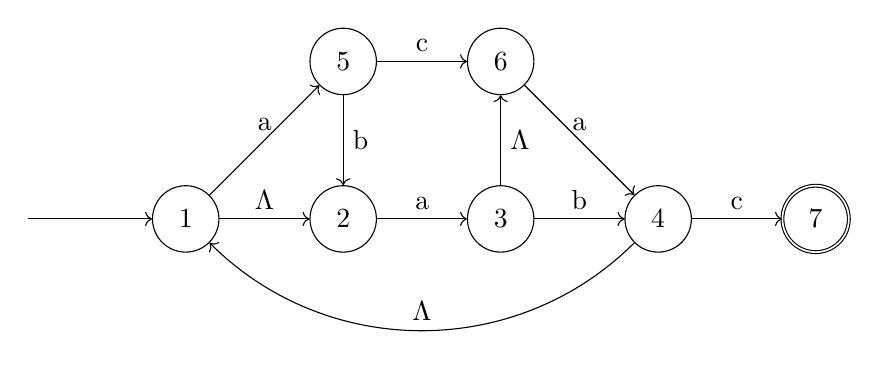
\begin{tikzpicture}
\fastart {0, 0};
\fanonterminalnode {2,0} {1};
\fanonterminalnode {4,0} {2};
\fanonterminalnode {6,0} {3};
\fanonterminalnode {8,0} {4};
\fanonterminalnode {4,2} {5};
\fanonterminalnode {6,2} {6};
\faterminalnode {10,0} {7};

\fatransition{start}{1}{};
\fatransition{1}{2}{$\Lambda$};
\fatransition{2}{3}{a};
\fatransition{3}{4}{b};
\farighttransition{3}{6}{$\Lambda$};
\fatransition{4}{7}{c};
\fatransition{1}{5}{a};
\fatransition{5}{6}{c};
\farighttransition{5}{2}{b};
\fatransition{6}{4}{a};
\faarctransition {4}{1}{$\Lambda$}{225}{315};

\end{tikzpicture}
} % end scaled box
\end{center}

Step~1 yields states 1 and 2, so this set becomes meta-state-$A$. There are three letters in the source language (a, b, c), so this yields the following rows:

\begin{center}
\small
\begin{tabular}{l|l|l|l}
\hline
\textbf{meta-state} & \textbf{NFA states} & \textbf{input} & \textbf{resulting states} \\
\hline
A & 1, 2 & a &  \\
A & 1, 2 & b &  \\
A & 1, 2 & c &  \\
\hline
\end{tabular}
\end{center}

Completing the first row, we can follow an $a$ from state 1 to 5, and from state 2 to 3. Add these two states to the resulting states column, and then follow the $\Lambda$s adding state 6. Label the set \code{ \{3, 5, 6\}} as meta-state~$B$ and add rows to the table:

\begin{center}
\small
\begin{tabular}{c|l|l|l|l}
\hline
& \textbf{meta-state} & \textbf{NFA states} & \textbf{input} & \textbf{resulting states} \\
\hline
1 & A & 1, 2 & a & B = 3, 5, 6 \\
2 & A & 1, 2 & b &  \\
3 & A & 1, 2 & c &  \\
4 & B & 3, 5, 6 & a &  \\
5 & B & 3, 5, 6 & b &  \\
6 & B & 3, 5, 6 & c &  \\

\hline
\end{tabular}
\end{center}

Completing rows 2 and 3, there are no $b$ nor $c$ transitions out of any of the states in meta-state~$A$, so the resulting states for both of these rows are empty.

Moving on to row 4, we can follow an $a$ from state 6 to state 4. We can then follow $\Lambda$s from 4 to 1 and 1 to 2 yielding meta-state $C$ containing states 1, 2, 4.

For row 5, we can follow a $b$ from 3 to 4 and from 5 to 2. We can then follow a $\Lambda$s from 4 to 1 and from there to 2 (which we've already reached), so this meta-state contains 1, 2 and 4, which we've already labeled $C$.

For row 6, we can follow a $c$ from 5 to 6. There are no $\Lambda$s from 6, so meta-state~$D$ contains only 6. Adding these new rows to the table, we have:

\begin{center}
\small
\begin{tabular}{c|l|l|l|l}
\hline
& \textbf{meta-state} & \textbf{NFA states} & \textbf{input} & \textbf{resulting states} \\
\hline
1 & A & 1, 2 & a & B = 3, 5, 6 \\
2 & A & 1, 2 & b & - \\
3 & A & 1, 2 & c & - \\
4 & B & 3, 5, 6 & a & C = 1, 2, 4 \\
5 & B & 3, 5, 6 & b & C \\
6 & B & 3, 5, 6 & c & D = 6 \\
7 & C & 1, 2, 4 & a & \\
8 & C & 1, 2, 4 & b & \\
9 & C & 1, 2, 4 & c & \\
10 & D & 6 & a & \\
11 & D & 6 & b & \\
12 & D & 6 & c & \\
\hline
\end{tabular}
\end{center}

Completing row 7, we can follow an $a$ from 1 to 5 and 2 to 3. The $\Lambda$ closure adds 6. This set of states is already labeled $B$, so we don't need to add any rows to the table.

For Row 8, there are no outbound edges on $b$ so the resulting states is empty.

For Row 9, we can follow a $c$ from 4 to 7. This new meta-state is labeled $E$.

\begin{center}
\small
\begin{tabular}{c|l|l|l|l}
\hline
& \textbf{meta-state} & \textbf{NFA states} & \textbf{input} & \textbf{resulting states} \\
\hline
1 & A & 1, 2 & a & B = 3, 5, 6 \\
2 & A & 1, 2 & b & - \\
3 & A & 1, 2 & c & - \\
4 & B & 3, 5, 6 & a & C = 1, 2, 4 \\
5 & B & 3, 5, 6 & b & C \\
6 & B & 3, 5, 6 & c & D = 6 \\
7 & C & 1, 2, 4 & a & B\\
8 & C & 1, 2, 4 & b & -\\
9 & C & 1, 2, 4 & c & E = 7 \\
10 & D & 6 & a & \\
11 & D & 6 & b & \\
12 & D & 6 & c & \\
13 & E & 7 & a & \\
14 & E & 7 & b & \\
15 & E & 7 & c & \\
\hline
\end{tabular}
\end{center}

For row 10, we can follow the a from 6 to 4 and then the $\Lambda$ to 1 and 2. This is already labeled~$C$.

For row 11, there are no outbound transitions on $b$, so the resulting states is empty.

For row 12, there are no outbound transitions on $c$, so the resulting states is empty.

\begin{center}
\small
\begin{tabular}{c|l|l|l|l}
\hline
& \textbf{meta-state} & \textbf{NFA states} & \textbf{input} & \textbf{resulting states} \\
\hline
1 & A & 1, 2 & a & B = 3, 5, 6 \\
2 & A & 1, 2 & b & - \\
3 & A & 1, 2 & c & - \\
4 & B & 3, 5, 6 & a & C = 1, 2, 4 \\
5 & B & 3, 5, 6 & b & C \\
6 & B & 3, 5, 6 & c & D = 6 \\
7 & C & 1, 2, 4 & a & B\\
8 & C & 1, 2, 4 & b & -\\
9 & C & 1, 2, 4 & c & E = 7 \\
10 & D & 6 & a & C\\
11 & D & 6 & b & -\\
12 & D & 6 & c & -\\
13 & E & 7 & a & \\
14 & E & 7 & b & \\
15 & E & 7 & c & \\
\hline
\end{tabular}
\end{center}

For Rows 13-15, there are no outbound edges from 7, so the resulting states are empty. This gives us the following table:

\begin{center}
\small
\begin{tabular}{c|l|l|l|l}
\hline
& \textbf{meta-state} & \textbf{NFA states} & \textbf{input} & \textbf{resulting states} \\
\hline
1 & A & 1, 2 & a & B = 3, 5, 6 \\
2 & A & 1, 2 & b & - \\
3 & A & 1, 2 & c & - \\
4 & B & 3, 5, 6 & a & C = 1, 2, 4 \\
5 & B & 3, 5, 6 & b & C \\
6 & B & 3, 5, 6 & c & D = 6 \\
7 & C & 1, 2, 4 & a & B\\
8 & C & 1, 2, 4 & b & -\\
9 & C & 1, 2, 4 & c & E = 7 \\
10 & D & 6 & a & C\\
11 & D & 6 & b & -\\
12 & D & 6 & c & -\\
13 & E & 7 & a & -\\
14 & E & 7 & b & -\\
15 & E & 7 & c & -\\
\hline
\end{tabular}
\end{center}

All rows are filled in, so we are done.

\textbf{Important note:} The procedure is to follow the input out of the NFA states and then follow the $\Lambda$s. A common mistake is to follow the $\Lambda$s out of the NFA states. For example, when filling out the last row, even though there is a $\Lambda$ from state 3, we don't follow it because we are only looking for transitions on $c$.

The subset construction was supposed to turn an NFA into a DFA, but it appears to have just produced a table. We can take the information in our final table from the example we just completed and summarize it in Figure~\ref{F.transitionTable}.

%----------------------------------------------------------
\begin{figure}[hbt]
\centering

\small
\begin{tabular}{l|l|l}
\hline
\textbf{From} & \textbf{transition on} & \textbf{To} \\
\hline
A & a & B \\
B & a & C \\
B & b & C \\
B & c & D \\
C & a & B\\
C & c & E \\
D & a & C \\
\hline
\end{tabular}
\caption[Transition table for DFA]{A summary of the table derived in this section. Each row contains the start state, and input character, and the resulting state if that character is found while in the start state.}
  \label{F.transitionTable}
\end{figure}
%----------------------------------------------------------

This is known as a transition table. It is fairly straight forward to convert this table into a DFA (and a DFA into a transition table). Create states for each state in the table (the union of the From and To columns). The start state is always $A$, and any meta-state that included a final state in the original NFA is a final state in the DFA (in this case State~$F$). The resulting DFA is as follows:

\begin{center}
\scalebox{.7}{
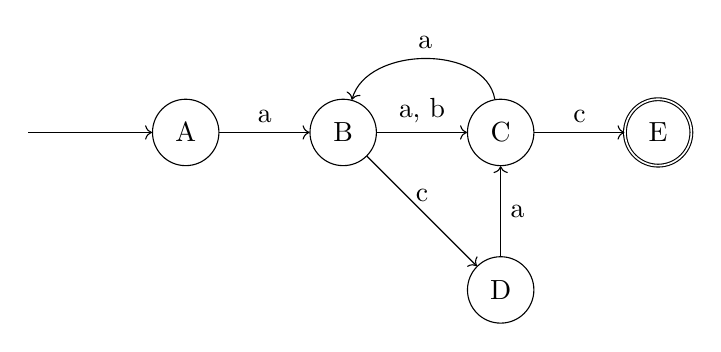
\begin{tikzpicture}
\fastart {0, 0};
\fanonterminalnode {2,0} {A};
\fanonterminalnode {4,0} {B};
\fanonterminalnode {6,0} {C};
\fanonterminalnode {6,-2} {D};
\faterminalnode    {8,0} {E};

\fatransition{start}{A}{};
\fatransition{A}{B}{a};
\fatransition{B}{C}{{a, b}}; 
\fatransition{B}{D}{c};
\faarctransition{C}{B}{a}{100}{75};
\fatransition{C}{E}{c};
%\fatransition{D}{C}{a};
%\faarctransition{B}{D}{b}{270}{180};
%\fatransition{B}{D}{b};
\farighttransition{D}{C}{a};
%\farighttransition{G}{C}{a,b};
%\faarctransition{D}{F}{c}{0}{270};
%\fatransition{D}{F}{c};
%\farighttransition{B}{E}{c};
%\fatransition{E}{C}{a};
%\faarctransition {C}{B}{a}{225}{315};

\end{tikzpicture}
} % end scaled box
\end{center}

Does the subset construction always result in a DFA, or might it result in another NFA? The answer is that it always results in a DFA for the following two reasons:
\begin{enumerate}
\item The \emph{input} column never has $\Lambda$s, so the resulting FA will not have any $\Lambda$ transitions.
\item When generating rows, each meta-state has exactly one row for each input character. As a result, there will never be multiple outbound transitions for the same character.
\end{enumerate}
The consequence is that the resulting FA has no non-determinism and is therefore a DFA.

\chapter{Theory}
\label{C.RL.theory}

What we have done so far:

We have shown that Thompson's Construction can turn any regular expression into an NFA. This implies that:
\begin{quote}
$L($regular expressions$) \subseteq L($NFA$)$
\end{quote}
This statement means that the set of all languages that can be constructed with regular expressions is a subset (or equal) of the languages that can be constructed with an NFA. In other words, anything that can be done with a regular expression can also be done with an NFA.

The Subset Construction showed that any NFA can be turned into a DFA. This implies that:
\begin{quote}
$L($NFA$) \subseteq L($DFA$)$
\end{quote}
So we now have:
\begin{quote}
$L($regular expressions$) \subseteq L($NFA$) \subseteq L($DFA$)$
\end{quote}

There are proofs both by induction and construction that show that any DFA can be turned into a regular expression. The proofs aren't particularly illuminating, so they won't be presented here. The statement will simply be taken on faith. So we now have:

\begin{quote}
$L($regular expressions$) \subseteq L($NFA$) \subseteq L($DFA$) \subseteq L($regular epxressions$)$
\end{quote}
The only way that this can be true is if:
\begin{quote}
$L($regular expressions$) = L($NFA$) = L($DFA$)$
\end{quote}
In other words, regular expressions, NFAs and DFAs are all equally powerful. They can be used to define exactly the same set of languages. This relation is known as Kleene's Theorem. It can be used to prove interesting properties of regular languages. Some properties are easier to prove using DFA's, some are easier to prove using regular expressions, but since these mechanisms are equivalent (can be used to define the same set of languages), then proving a property using one mechanism means the property applies to all languages in the family.

\begin{theorem}
The union of two regular languages is regular.
\end{theorem}
This can be proved by construction. Consider two languages $L_1$ and $L_2$ both of which are regular. Since they are regular, there is a DFA that corresponds to each of them. If we construct a new NFA by creating a new start state that is connected to the start states of both $L_1$ and $L_2$, we would have an NFA that accepts any word in $L_1$ or any word in $L_2$. Since we have an NFA for this language, the language must be regular. Figure~\ref{F.union.re} illustrates this in picture form.

%----------------------------------------------------------
\begin{figure}[hbt]
\centering
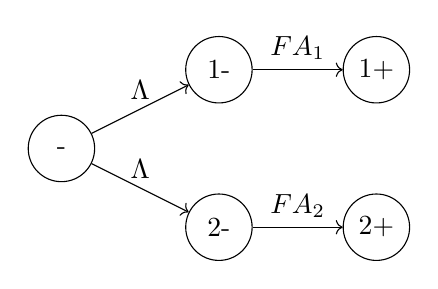
\begin{tikzpicture}

\fanonterminalnode {-2,0}{-};
\fanonterminalnode {0,1}{1-};
\fanonterminalnode {0,-1}{2-};
\fanonterminalnode {2, 1}{1+};
\fanonterminalnode {2, -1}{2+};

\fatransition{-}{1-}{$\Lambda$};
\fatransition{-}{2-}{$\Lambda$};
\fatransition{1-}{1+}{$FA_1$};
\fatransition{2-}{2+}{$FA_2$};

\end{tikzpicture}
\caption[Union of to regular expressions]{This FA accepts the strings accepted by $FA_1 \cup FA_2$}
\label{F.union.re}
\end{figure}
%----------------------------------------------------------
This could also be proved using regular expressions. If $RE_1$ is a regular expression that defines $L_1$, and $RE_2$ is a regular expression that defines $L_2$, then $RE_1 + RE_2$ defines the language $FA_1 \cup FA_2$.

\begin{theorem}
The complement of any regular language is regular.
\end{theorem}
First, what do we mean by the complement of a language. If a regular language $L$ is defined over the alphabet $\Sigma$, then the complement of $L$, which we will call $L'$, is the set of all strings that are in $\Sigma ^*$, but not in $L$.

We can again prove this by construction. If $L$ is regular, then there is a complete DFA that generates the language. By ``complete'', we mean that every state has an outbound transition for every letter in $\Sigma$. If we take that DFA and reverse the ``plusness'' of each state (that is, every state that was a final state in the original becomes a non-final state in the result, and any state that was non-final in the original becomes final in the result) then any string accepted by the original will be rejected in the final and any string regected by the original will be accepted in the final. Since the DFA is complete, it will never ``crash'' - that is, for each input letter, it will always have a transition it can follow. Since it is a deterministic FA, a given input can only wind up in a single state. That one an only state has opposite implications in the two FAs. If it accepts the string in one, it rejects the string in the other. As a result, the two FAs represent languages that are complements of each other.

%----------------------------------------------------------
\begin{figure}[htb]
\centering

%\scalebox{.7}{
\begin{subfigure}[b]{0.45\textwidth}
\centering
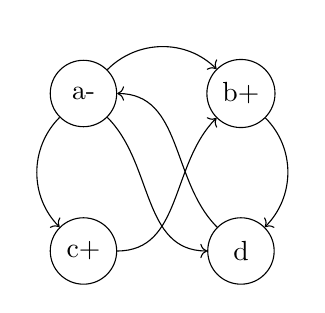
\begin{tikzpicture}

\fanonterminalnode {0,2} {a-};
\fanonterminalnode {2,2} {b+};
\fanonterminalnode {0,0} {c+};
\fanonterminalnode {2,0} {d};

\faarctransition {a-}{b+}{}{45}{135};
\faarctransition {a-}{c+}{}{225}{135};
\faarctransition {a-}{d}{}{315}{180};
\faarctransition {b+}{d}{}{315}{45};
\faarctransition {d}{a-}{}{135}{0};
\faarctransition {c+}{b+}{}{0}{225};

%\node at (5,-1) {Concatenation};
%\node at (5,-2) {};
\end{tikzpicture}
\caption{Original FA}
\end{subfigure}
%}
~
\begin{subfigure}[b]{0.45\textwidth}
\centering
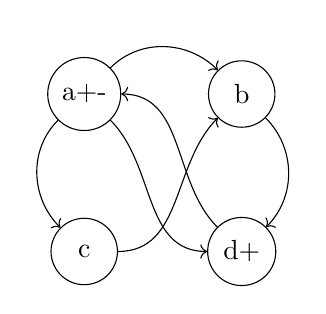
\begin{tikzpicture}

\fanonterminalnode {0,2} {a+-};
\fanonterminalnode {2,2} {b};
\fanonterminalnode {0,0} {c};
\fanonterminalnode {2,0} {d+};

\faarctransition {a+-}{b}{}{45}{135};
\faarctransition {a+-}{c}{}{225}{135};
\faarctransition {a+-}{d+}{}{315}{180};
\faarctransition {b}{d+}{}{315}{45};
\faarctransition {d+}{a+-}{}{135}{0};
\faarctransition {c}{b}{}{0}{225};

%\node at (5,-1) {Concatenation};
%\node at (5,-2) {};
\end{tikzpicture}
\caption{Compliment FA}
\end{subfigure}
%}

 \caption[Complement of a Regular Language]{A complete DFA can be modified to generate the complement of the original language by changing the ``plussness'' of each node: Final nodes in the original become non-final in the converted diagram and non-final nodes in the original become final nodes in the converted diagram.}
  \label{F.RL.Compliment}
\end{figure}
%----------------------------------------------------------

\begin{theorem}
The intersection of two regular languages is regular.
\end{theorem}

DeMorgan's Law for sets states that $L_1 \cap L_2 = (L_1' \cup L_2')'$. In other words, the intersection of two sets is equal to the complement of the union of the complement of the two sets. If $L_1$ and $L_2$ are regular then so are their complements ($L_1'$ and $L_2'$). Since these are regular, then so is their union ($L_1' \cup L_2'$). And finally, so is the complement of that language ($(L_1' \cup L_2')'$). Since this is equivalent of the intersection of the two languages, then the intersection must also be regular.

\begin{theorem}
There is an algorithm to determine if two regular expressions are equivalent.
\end{theorem}
Consider $L_1 = L(RE_1)$ and $L_2 = L(RE_2)$. If $RE_1$ and $RE_2$ define different languages, then either $L_1$ contains words not in $L_2$ or $L_2$ contains words not in $L_1$ (or both).
Since $L_1$ and $L_2$ are regular, we can compute $L_3 = (L_1 \cap L_2') \cup (L_1' \cap L_2)$. The first term in $L_3$ is all strings that are in $L_1$ but not in $L_2$. The second term is all strings that are in $L_2$ but not in $L_1$. If the union of those two terms is empty, then the two languages $L_1$ and $L_2$ must be equivalent.

But now we need a decision procedure for ``Is the language empty?''. If we have a regular expression for a language, then the following procedure will give one word in the language:
\begin{enumerate}
\item Delete all stars
\item If a $\Lambda$ is part of an alternation, remove that part of the alternation.
\item Delete all remaining $\Lambda$'s
\item For every alternation, keep only the left-most option
\item Remove parenthesis
\end{enumerate}
What is left must be a word in the language.

If we have an FA for the language, then the following procedure will determine if the FA accepts at least one word:
\begin{enumerate}
\item Add the start state to a work list
\item Remove a state from the work list and mark it as visited. Add all unmarked states reachable from this state to the work list.
\item Repeat Step~2 until the work list is empty.
\item If a final state was marked, then the language includes at least one word.
\end{enumerate}

\begin{theorem}
\label{T.FA.length}
Let F be an FA with N states. If F accepts any words at all, then it must accept a word of length less than N.
\end{theorem}
The shortest path from the start state to an accept state must visit each node at most once. As a result, if there is any path from the start state to an accept state, there must be a path with length less than N.

Theorem~\ref{T.FA.length} leads to another decision process for ``Is the language empty?'': Enumerate all words of length less than N (the number of states in the FA), and try them all. If the FA accepts any words, it must accept one of these words.

\begin{theorem}
Any infinite regular language must have a loop in the FA.
\end{theorem}
By ``loop in the FA'', what we mean is that there is some set of states which can be repeated an arbitrary number of times. For example, the states 2,3,4 in Figure~\ref{F.FA.loop} form a loop that can be repeated any number of times. 
%----------------------------------------------------------
\begin{figure}[hbt]
\centering
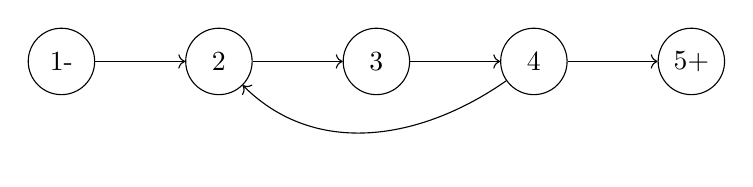
\begin{tikzpicture}

\fanonterminalnode {0,0}{1-};
\fanonterminalnode {2,0}{2};
\fanonterminalnode {4,0}{3};
\fanonterminalnode {6,0}{4};
\fanonterminalnode {8,0}{5+};

\fatransition{1-}{2}{};
\fatransition{2}{3}{};
\fatransition{3}{4}{};
\fatransition{4}{5+}{};
\faarctransition {4}{2}{}{215}{315};

\end{tikzpicture}
\caption[FA with a loop]{This FA represents an infinite language, and it contains a loop composed of states 2,3,4.}
\label{F.FA.loop}
\end{figure}
%----------------------------------------------------------
Consider any infinite regular language $L$. The language $L$ can be generated by some DFA. The DFA is finite, so let's say it has $N$ states, where $N$ is some finite number. The longest string that can be generated by this DFA without visiting the same state more than once is $\le (N-1)$. Clearly the length can't be $\ge N$ because if you make $N$ transitions between $N$ states, then at least one of those states must be repeated. The maximum length might be $< (N-1)$ because there might not be any path that touches each state exactly once. Since the maximum length without repeating states is $\le (N-1)$, then any string longer than this must visit the same state at least twice. In other words, there must be a path from State $S_i$ back to State $S_i$ and from there to a final state. This path constitutes a loop. As a result, the FA for any infinite regular language must contain a loop.

\begin{lemma}
\label{T.RL.pumping.lemma}
Let $L$ be any infinite regular language, then there exist strings $x,y,z$, where $y$ is not the empty string, such that all strings $x y^n z$ with $n>0$ are in $L$.
\end{lemma}

Since there are an infinte number of words in $L$, any FA that generates $L$ must have a loop. The string $x$ represents the path from the start state to the beginning of the loop. The string $y$ represents the path around the loop. The string $z$ represents the path from the end of the loop to a final state. Since $y$ represents a loop, then each circuit around the loop generates another $y$. Since the loop can be traversed an arbitrary number of times, strings with an arbitrary number of $y$'s can be generated. This is shown in Figure~\ref{F.RL.pumping.lemma}.

%----------------------------------------------------------
\begin{figure}[hbt]
\centering
\begin{tikzpicture}

\fanonterminalnode {0,0}{1-};
\fanonterminalnode {2,0}{2};
\fanonterminalnode {4,0}{3+};

\fatransition{1-}{2}{x};
\fatransition{2}{3}{z};
\falooptop {2}{y};

\end{tikzpicture}
\caption[FA illustrating the pumping lemma]{This FA illustrates the proof of the pumping lemma. The strings $x,y,z$ are labeled. Clearly each circuit of the loop generates another $y$.}
\label{F.RL.pumping.lemma}
\end{figure}
%----------------------------------------------------------


Lemma~\ref{T.RL.pumping.lemma} is known as the Pumping Lemma for Regular Languages. It can be used to prove that a language is NOT regular. Before giving some examples, it is important to make several clarifications:
\begin{enumerate}
\item The Lemma states that all strings $x y^n z$ are in $L$. It does NOT say that all strings in $L$ are in the form $x y^n z$.
\item The Lemma can be used to prove that a language is NOT regular. It cannot be used to prove that a language IS regular. In other words, there are some non-regular languages the fit the form of the pumping lemma, but any language that is infinite that does NOT fit the pumping lemma must not be regular.
\end{enumerate}

Consider the language $ab^*c$. This is an infinite language and it is regular, so it must conform to the pumping lemma. To show this, take $x=a$, $y=b$, $z=c$. With this assignment, it should be clear that all strings $xy^n z$ are in the language.

Now let's consider the language of all strings that consist of any number of $a$'s followed by any number of $b$'s. This language can be represented as $a^n b^m$. Is this language regular? Let's see if we can prove it is NOT regular using the pumping lemma. Let's take $x=a$, $y=ab$, $z=b$. The string $xyz$ is $aabb$ which is in the language. However, the string $xy^2 z$ is $aababb$ which is NOT in the language. Can we conclude from this that the language is not regular? No.

The previous paragraph gave a single example of a choice for $x, y, z$, and a single example is not a proof. To use the pumping lemma to prove a language is not regular, you must show that there is no possible choice of $x, y, z$ where the pumping lemma applies. Let's consider another choice. Let's choose $x=a$, $y=a$, $z=b$. With this choice, any $xy^n z$ can be written $a^{n+1} b$, all of which are in the language. Note that this does not represent ALL words in the language, but all words of this form ARE in the language. 

Since we found strings $x, y, z$ for which all $xy^nz$ are in the language, we failed to prove that this language is not regular. This should come as no surprise since the since the regular expression $a^*b^*$ generates this language. Since there is a regular expression that generates the language, the language must be regular.

Now let's make a minor modification to our language. Instead of any number of $a$'s followed by any number of $b$'s, let's require the $a$'s to be followed by the same number of $b$'s. This language can be expressed $a^nb^n$. Note that this time both letters have the same superscript meaning there must be the same number of each. Can we find an $x, y, z$ such that all strings $xy^nz$ are in the language.

\begin{quote}
Possibility 1: $y$ consists only of $a$'s. In this case, increasing $n$ in $xy^nz$ would increase the number of $a$'s without increasing the number of $b$'s thus generating words not in the language.

Possibility 2: $y$ consists only of $b$'s. In this case, increasing $n$ in $xy^nz$ would increase the number of $b$'s without increasing the number of $a$'s thus generating words not in the language.

Possibility 3: $y$ consists of both $a$'s and $b$'s. In this case, increasing $n$ in $xy^nz$ would increase the number of $a$-$b$ transitions. Since the language only allows one $a-b$ transition, this would generate words not in the language.

Since $y$ cannot be the empty string, we've enumerated all possible choices for $y$ and none of them meet the requirements of the pumping lemma. We can therefore conclude that $a^nb^n$ is not regular.
\end{quote}

This language is of more than passing concern. Consider the substitution where instead of $a$ we have an open parenthesis and instead of $b$ we have a closing parenthesis. The language is now $(^n )^n$, which is the set of nested parenthesis. The ability to have an arbitrary number of nested parenthesis (or curly braces) is an artifact of many programming languages. The fact that you cannot generate this language with a regular expression means that the syntax of most programming languages is not regular. It also means that the syntax for regular expressions is not itself regular.

If we assume that the syntax for programming languages is formal (and it would be difficult to write a compiler if it was not: how could you decide if a source file was a valid program if the language was not formal?), then we need another class of languages to express the syntax of programming languages. This other set of languages is the subject of the next part of this book.

\needsproblems

%%%%%%%%%%%%%%%%%%%%%%%%%%%%%%%%%%%%%%%%%%%%%%%
%%%%%%%%%%%%%%%% CFGs %%%%%%%%%%%%%%%%%%%%%%%%%
%%%%%%%%%%%%%%%%%%%%%%%%%%%%%%%%%%%%%%%%%%%%%%%
\part{Context Free Grammars}

\chapter{Context Free Grammars}
With English, there is a progression of language elements:
\begin{quote}
Letters $\rightarrow$ Words $\rightarrow$ Sentences $\rightarrow$ Paragraphs
\end{quote}
With computers, there is a similar progression:
\begin{quote}
Characters $\rightarrow$ Tokens $\rightarrow$ Programming Languages $\rightarrow$ Algorithms
\end{quote}

Regular expressions are suitable for defining tokens (such as integer constants or identifiers), but they can't be used for defining most programming languages because most programming languages have nesting features (parenthesis, curly braces, etc.), and regular languages are incapable of defining such features. 

In this part of the book we examine another category of languages: Context Free Languages. These languages are capable of expressing nesting, and they are suitable for defining most programming languages.

\section{Introduction to CFGs}
Recall that nested parenthesis cannot be represented as a regular expression. Another example that fits the same pattern as nested parenthesis is shown in Listing~\ref{L.infinite.ifs}
\begin{lstlisting}[caption={Nested if statements},label=L.infinite.ifs]
if (x)
{
   if (x)
	 {
	    if (x)
			{
			   etc.
			}
	 }
}
\end{lstlisting}
Each of these nesting problems boils down to the language $a^nb^n$, which we've shown cannot be represented with a regular expression. This pattern can, however, be represented with a recursive definition:
\begin{enumerate}
\item $\Lambda$ is in BAL
\item if $x$ is in BAL, then so is $axb$
\end{enumerate}

This suggests that languages defined recursively are more powerful (in the sense that they can define more languages) than regular expressions. We want to formalize the structure of recursive definitions so that we can prove properties of these languages much as we did for regular languages in Chapter~\ref{C.RL.theory}. Context Free Grammars are one such formalization.

A Context Free Grammar (CFG) is made up a a list of productions of the general form:
\begin{quote}
X can be replaced by A B C
\end{quote}
Where the X, A, B, C can be thought of as variables. The potential for recursion comes about because the variable being replaced (X in this example) can appear in the replacement:
\begin{quote}
X can be replaced by A X C
\end{quote}

More formally, a production in a CFG consists of a left hand side and a right hand side. The left hand side gives the symbol that can be replaced. The right hand side gives the list of symbols that can replace that symbol. The two sides are typically separated 
either by an arrow ( $\rightarrow$ ) 
or sometimes a colon-colon-equals ( ::= ). 
A sample production that indicates that the symbol \code{A} 
can be replaced by \code{X Y Z} is given below:

\cfgindentprod{A}{X Y Z}

Symbols in CFGs are of two flavors: non-terminals are those that appear on the left hand side of a production. They are non-terminals because they can be replaced by other symbols. Terminals are those symbols that never appear on the left hand side. They are ``terminal'' because they can never be replaced. For ease of reading, non-terminals are usually given in \texttt{UPPERCASE}, and terminals are given in \texttt{lowercase}. CFGs also need a start symbol: the symbol that is the starting point for derivations. The start symbol is often either \code{S} or \code{START}, but if neither is specified, the left hand side of the first production is assumed to be the start symbol.

%----------------------------------------------------------
\begin{cfg}{A CFG that defines the language of any number of \code{a}'s followed by the same number of \code{b}'s.}{F.cfg.1}
Q\cfgprod{S}{a S b}Q
Q\cfgprod{S}{$\Lambda$}Q
\end{cfg}
%----------------------------------------------------------

Figure~\ref{F.cfg.1} shows a complete CFG. The productions have been numbered for easy reference. There are only two productions. The first one says that the start symbol (\code{S}) can be replaced with ``\code{a S b}''. Note that this is a recursive rule because the \code{S} appears on both sides. The second production says that \code{S} can be replaced with nothing.

What can we do with this CFG? Let's do some derivations. Starting with the start symbol and Production 1, we can get the string \code{aSb}. If we then use Production 2, we are left with the string \code{ab}. Since there are no more non-terminals, we are done.

What if we invoked Production 1 more than once? The first invocation produces \code{aSb}. The next invocation produces \code{aaSbb}. Each invocation adds another \code{a} and \code{b}. When we finally invoke Production 2, we are left with a string of \code{a}'s followed by the same number of \code{b}'s.

While not the most complex illustration, this CFG illustrates that CFGs are more powerful than regular expressions\footnote{Technically, we've only shown that CFGs can solve one problem that regular expressions can't. It remains to be shown that everything you can do with a regular expression you can also do with a CFG. Once we show that, we can conclude that CFGs are strictly more powerful than regular expressions.}. Regular expressions are not able to generate balanced parenthesis. A regular expression such as $(^*)^*$ allows any number of opening parenthesis and any number of closing parenthesis, but there is no way to guarantee that the number of closing parenthesis match the number of opening parenthesis. If we substituted parenthesis for the \code{a} and \code{b} in Figure~\ref{F.cfg.1}, we would have a solution to the balanced parenthesis problem.

Figure~\ref{F.cfg.2} presents a more interesting CFG. This language defines a program as zero or more statements. An individual statement can be an assignment statement (in this language, an assignment statement is a terminal, so the assumption is that they are defined elsewhere), an \code{if} statement, or a compound statement (curly braces surrounding any number of statements). 

%----------------------------------------------------------
\begin{cfg}{This CFG defines a program as being zero or more statements, where each statement is either an \code{if} statement, an assignment statement or a compound statement.}{F.cfg.2}
Q\cfgprod{PROGRAM}{STMTS}Q
Q\cfgprod{STMTS}{STMT STMTS}Q
Q\cfgprod{STMTS}{$\Lambda$}Q
Q\cfgprod{STMT}{IF\_STMT}Q
Q\cfgprod{STMT}{COMPOUND\_STMT}Q
Q\cfgprod{STMT}{assignment\_stmt}Q
Q\cfgprod{IF\_STMT} {if ( expr ) STMT}Q
Q\cfgprod{COMPOUND\_STMT} { \{ STMTS \} }Q
\end{cfg}
%----------------------------------------------------------

The program in Listing~\ref{L.nested.ifs} illustrates the features of the language defined by the CFG in CFG~\ref{F.cfg.2}. Line~1 is a simple assignment statement. The \code{if} statement that begins in Line~2 is a simple \code{if} statement. The \code{if} statement that begins in Line~4 shows a nested \code{if} statement. The compound statement that begins in Line~8 shows that compound statements can be nested and that they can be empty (in Line~11).

\begin{lstlisting}[caption={Sample program in the language defined by the CFG in CFG~\ref{F.cfg.2}},label=L.nested.ifs]
assignment_statement
if (expr)
   assignment_statement
if (expr)
    if (expr)
       assignment_statement
if (expr)
{
   assignment_statement
   assignment_statement
   {
   }
}
\end{lstlisting}

\section{Derivations}

Listing~\ref{L.nested.ifs} claims to be a program in the language defined in Figure~\ref{F.cfg.2}. How can we substantiate this claim? This is normally done by showing a derivation of the program given the CFG. Each line of a derivation substitutes a single non-terminal for the right-hand-side of a production for that non-terminal. 

Derivations start with the start symbol and continue until there are only terminals. Each step other than the first should list the production number that was invoked to make the substitution. Rather than starting with the longer program in Listing~\ref{L.nested.ifs}, let's start with the shorter program in Listing~\ref{L.short.prog}.

\begin{lstlisting}[caption={Short program program in the language defined by the CFG in CFG~\ref{F.cfg.2}. The derivation of this program is given in Derivation~\ref{D.derive.1}},label=L.short.prog]
if (expr)
{
   assignment_statement
   assignment_statement
}
\end{lstlisting}

\begin{derivation}{Derivation of the program in Listing~\ref{L.short.prog}}{D.derive.1}
    PROGRAM
1   STMTS
4   IF_STMT
7   if ( expr ) STMT
8   if ( expr ) { STMTS }
2   if ( expr ) { STMT STMTS }
6   if ( expr ) { assignment_stmt STMTS }
2   if ( expr ) { assignment_stmt STMT STMTS }
6   if ( expr ) { assignment_stmt assignment_stmt STMTS }
3   if ( expr ) { assignment_stmt assignment_stmt }
\end{derivation}

The derivation in Derivation~\ref{D.derive.1} is what's known as a left-most derivation because each time there were multiple non-terminals, the left-most one was replaced. It is also possible to do right-most derivations, and you can also do neither: sometimes pick the left-most non-terminal, sometimes the right-most, and sometimes one in the middle.

\subsection{Derivation forms}\label{S.derive.forms}
The left-most nature of Derivation~\ref{D.derive.1} wasn't that obvious because there were never more than two non-terminals in any line of the derivation. For a better example, consider the the CFG for expressions in postfix notation given in CFG~\ref{CFG.postfix}. Using that grammar, Derivation~\ref{D.post.top.down} shows a derivation of the expression
\begin{quote}
3 4 + 5 6 - *
\end{quote}
%----------------------------------------------------------
\begin{cfg}{This CFG defines the syntax for postfix expressions. In production 4, the vertical bars represent alternation, so an OP can be one of the four arithmetic operators.}{CFG.postfix}
Q\cfgprod{EXPR}{POST}Q
Q\cfgprod{POST}{POST POST OP}Q
Q\cfgprod{POST}{number}Q
Q\cfgprod{OP}{+ | - | * | /}Q
\end{cfg}
%----------------------------------------------------------

\begin{derivation}{Derivation of the expression 3 4 + 5 6 - *}{D.post.top.down}
    EXPR
1   POST
2   POST POST OP
2   POST POST OP POST OP
3   3 POST OP POST OP
3   3 4 OP POST OP
4   3 4 + POST OP
2   3 4 + POST POST OP OP
3   3 4 + 5 POST OP OP
3   3 4 + 5 6 OP OP
4   3 4 + 5 6 - OP
4   3 4 + 5 6 - *
\end{derivation}
Derivation~\ref{D.post.top.down} is both top-down and left-most. It is top-down because it begins with the start symbol and progresses to all terminals. When a derivation is represented graphically (see Section~\ref{S.syntax.trees}), this derivation starts at the top of the diagram and progresses to the bottom. This derivation is also left-most because in each step, the left-most non-terminal is the one that was replaced.

Derivation~\ref{D.post.bottom.up} shows a bottom-up right-most derivation of the same expression. It is bottom up because it begins with all terminals and combines them using productions until the terminals have been reduced to the start symbol. Note that if these steps were reversed, the derivation would be top-down. In this sense, top-down and bottom-up derivations are inverses of each other. Note also that if this derivation was inverted to its top-down form, it would be a right-most derivation. In each step it is the right-most non-terminal that gets replaced. The left-most or right-most nature of a derivation is always from the top-down perspective.
\begin{derivation}{Bottom-up right-most Derivation of the expression 3 4 + 5 6 - *}{D.post.bottom.up}
    3 4 + 5 6 - *
3   POST 4 + 5 6 - *
3   POST POST + 5 6 - *
4   POST POST OP 5 6 - *
2   POST 5 6 - *
3   POST POST 6 - *
3   POST POST POST - *
4   POST POST POST OP *
2   POST POST *
4   POST POST OP
2   POST
1   EXPR
\end{derivation}

We now have four derivation forms: top-down left-most, top-down right-most, bottom-up left-most, and bottom-up right-most. The first and last of these are the most common, and the ones most often used by compilers. 

One last thing to note: If you were asked to give a derivation of an expression using our postfix grammar, there would be many correct answers. You could chose which order to invoke productions and which non-terminal to replace in each step. But if any of the four flavors mentioned in the previous paragraph were requested, there would be exactly one correct answer. There would be no choice as to which non-terminal to replace or which production to invoke. 

The only-one-right-derivation property is true of this grammar because it is non-ambiguous. Ambiguous grammars will be described in Section~\ref{S.ambiguous.grammars}.

\subsection{Syntax Trees}\label{S.syntax.trees}
Derivations can be represented graphically as syntax trees. In a syntax tree, the children of each non-terminal are the items from the right hand side of the production that was used to replace the non-terminal. Figure~\ref{F.syntax.tree.1} shows the syntax tree for the derivation in Derivation~\ref{D.derive.1}.
\begin{figure}[htb]
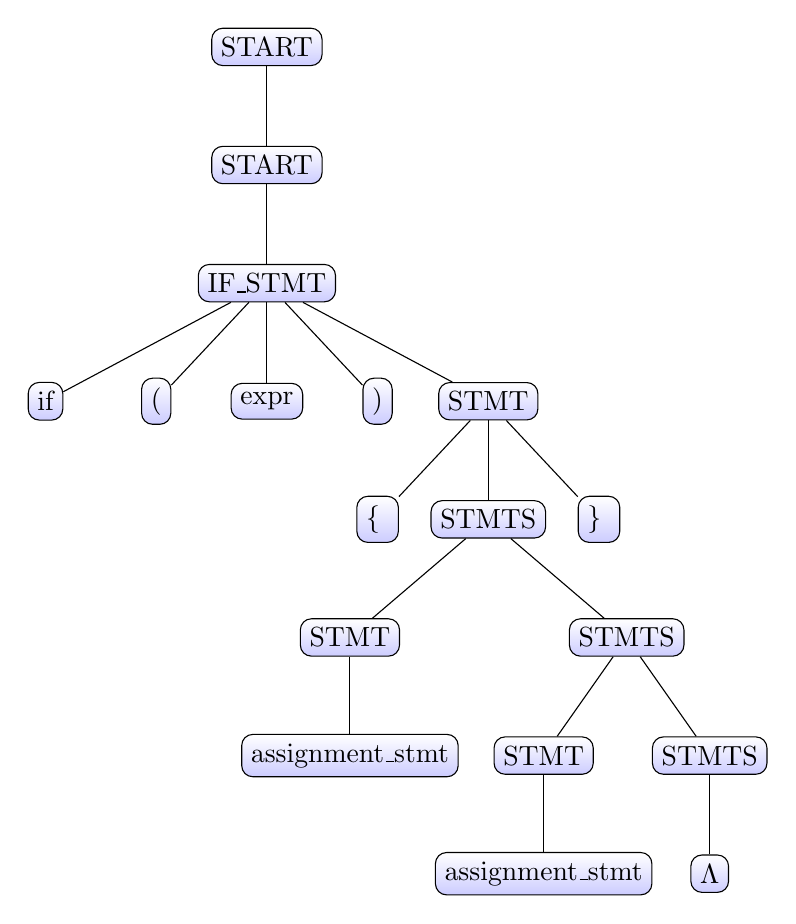
\begin{tikzpicture}[sibling distance=4em, 
  level 5/.style={sibling distance=10em},
  level 6/.style={sibling distance=6em},
  every node/.style = {shape=rectangle, rounded corners,
    draw, align=center,
    top color=white, bottom color=blue!20}]]
  \node {START}
    child { node {START} 
      child { node {IF\_STMT}
        child { node {if} }
				child { node {(} }
				child {node {expr} }
				child { node {)} } 
				child { node {STMT}
				  child { node { \{ } }
					child { node {STMTS} 
					  child { node {STMT} 
						  child {node {assignment\_stmt} }
						}
						child { node {STMTS}
					    child { node {STMT} 
						    child {node {assignment\_stmt} }
						  }
						  child { node {STMTS}
							 child { node {$\Lambda$} }
							}
						}
					}
					child { node { \} } }
				}
			}
		};
\end{tikzpicture}
\caption[Syntax tree]{A syntax tree representing the derivation in Figure~\ref{D.derive.1}.}
\label{F.syntax.tree.1}
\end{figure}
Note that if the derivation is given in tree form, there is no sense of left-most or right-most because the tree gives no indication of what order the productions were invoked. For the derivation represented in Figure~\ref{D.derive.1}, it would not matter what order the productions were invoked. All derivations would produce an identical tree. The only-one-tree property is true because the grammar used for this derivation is non-ambiguous. Ambiguous grammars are discussed in the next section.

\section{Ambiguous Grammars}\label{S.ambiguous.grammars}
English, and I presume all spoken languages, is ambiguous. A single statement can be interpreted different ways. Consider the two statements
\begin{quote}
Fruit flies like an apple.
Time flies like an arrow.
\end{quote}
Both statements appear structurally the same; only a couple of words were changed. However, with the normal interpretations, ``flies'' is the subject in the first sentence, but the verb in the second (unless the second sentence is referring to flies native to the Tardis). If we are sufficiently familiar with the English language, we come up with the correct interpretation of each sentence without even consciously thinking about it. But what if you tried to write a program to understand English? How would it distinguish betweeen the two.

Consider the statement, ``I shot the man with the gun.'' When the police show up and you utter that sentence, you hope they interpret it as, ``See that man over there with a gun? I shot him in self defence.'' You hope they don't interpret it, ``See this gun in my hand? I shot that [possibly unarmed] man over there with this gun.'' Although I hope you never find youself in a situation where you have to utter such a sentence, if you do, you might want to pick a less ambiguous statement.

A grammar is ambiguous when a single input can produce multiple different meanings. For CFGs, the ``meanings'' are defined by the syntax tree produced by parsing a statement. The grammar in CFG~\ref{F.GR.ambiguous} illustrates this. The expression $3+4*5$ can be derived two different ways. One has the multiplication happening first and the other with the addition happening first. These two derivations are illustrated by the trees in Figure~\ref{D.derive.2}.
%----------------------------------------------------------
\begin{cfg}{An ambiguous expression grammar.}{F.GR.ambiguous}
Q\cfgprod{EXPR}{EXPR + num}Q
Q\cfgprod{EXPR}{EXPR * num}Q
Q\cfgprod{EXPR}{num}Q
\end{cfg}
%----------------------------------------------------------
%----------------------------------------------------------
\begin{figure}[htb]
\centering
%\scalebox{.7}{
\begin{subfigure}[b]{0.95\textwidth}
\centering
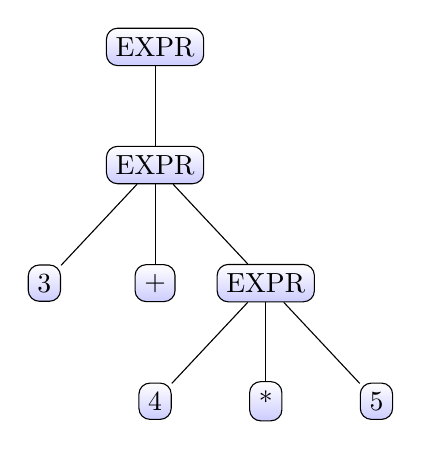
\begin{tikzpicture}[sibling distance=4em, 
  every node/.style = {shape=rectangle, rounded corners,
    draw, align=center,
    top color=white, bottom color=blue!20}]]
  \node {EXPR}
    child { node {EXPR} 
		  child { node {3}}
			child { node {+}}
      child { node {EXPR}
        child { node {4} }
				child { node {*} }
				child { node {5} }
			}
		};
\end{tikzpicture}
\caption{Derivation showing multiplication happening first.}
\end{subfigure}
%%%%%%

\begin{subfigure}[b]{0.95\textwidth}
\centering
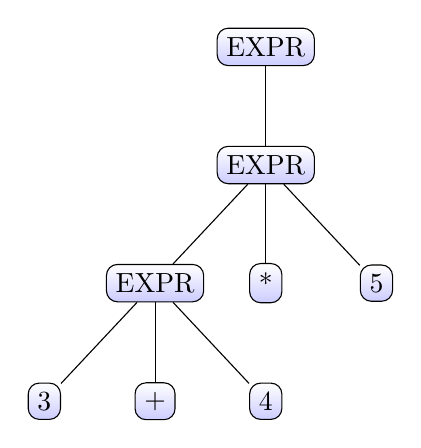
\begin{tikzpicture}[sibling distance=4em, 
  every node/.style = {shape=rectangle, rounded corners,
    draw, align=center,
    top color=white, bottom color=blue!20}]]
  \node {EXPR}
    child { node {EXPR} 
      child { node {EXPR}
  		  child { node {3}}
	  		child { node {+}}
        child { node {4} }
			}
			child { node {*} }
			child { node {5} }
		};
\end{tikzpicture}
\caption{Derivation showing addition happening first.}
\end{subfigure}
%%%%%%

 \caption[Derivations from an ambiguous grammar]{Two syntax trees showing derivations of $3+4*5$ using the ambiguous grammar in CFG~\ref{F.GR.ambiguous}}
\label{D.derive.2}
\end{figure}
%----------------------------------------------------------

Note that the ambiguity of a grammar is defined by the existence of multiple trees for the same expression. It is not defined based on different derivation orders for the same expression. Recall that when a derivation is represented as a tree, the top-down vs. bottom-up and left-most vs. right-most nature of the derivation is obscured. Any grammar can be used in a left-most or right-most (or middle-most) fashion. That does not mean the grammar is ambiguous (otherwise, all grammars would be). If each of these derivations results in the same tree, the grammar is considered non-ambiguous.

For programming languages, ambiguous grammars are clearly bad. The expression $3+4*5$ should not evaluate to a different value simply because the compiler did a left-most derivation versus a right-most derivation. There are expression grammars that resolve the ambiguity of the grammar in Figure~\ref{F.GR.ambiguous}, but since this is a theory book, we will leave that topic for a compiler book.

\section {Grammar Forms}
One of the tasks of a compiler is to find a derivation of the input (the source code being compiled) given the definition of the language (typically expressed as a CFG). This part of a compiler is known as a parser. In order for a parser to be efficient, there needs to be turn-the-crank algorithms for finding a derivation. The algorithms should not require a guess-and-check process. In particular, given the next $N$ input symbols, the parser should always know what production to use next in the derivation.

There are two primary algorithms used by parsers. One is a top-down algorithm, the other is a bottom-up algorithm. The top-down algorithm starts with the start symbol and based on the next input token invokes a production. This continues until all input is exhausted and only terminals remain. The bottom-up algorithm reads tokens and periodically reduces some collection of symbols that match the right hand side of a production to the symbol on the left hand side of that production. This continues until all input is exhausted and only the start symbol remains.

There are two grammar forms that are used in support of these compilers. An LL(1) grammar reads input Left to right (the first L), does a Left-most derivation (the second L), and can always make a decision with 1 token of look-ahead. An LR(1) grammar reads input Left to right, does a Right-most derivation and can always make a decision with 1 token of look-ahead. LL(1) grammars are used by top-down parsers, and LR(1) grammars are used by bottom-up parsers.

These grammars are related as follows.
\begin{quote}
$LL(1) \subset LR(1) \subset CFG$
\end{quote}
Note that these are strict subsets. There are things that can be done with an LR(1) grammar that cannot be done with an LL(1) grammar. An there are things that can be done with CFGs that cannot be done with an LR(1) grammar.

To illustrate what causes difficulties with the top-down algorithm (and therefore the restrictions placed on LL(1) grammars), consider the grammar given in CFG~\ref{C.paren.expr}. %----------------------------------------------------------
\begin{cfg}{This CFG defines a fully parenthesized expression.}{C.paren.expr}
Q\cfgprod{EXPR}{number}Q
Q\cfgprod{EXPR}{(EXPR + EXPR)}Q
Q\cfgprod{EXPR}{(EXPR - EXPR)}Q
Q\cfgprod{EXPR}{(EXPR / EXPR)}Q
Q\cfgprod{EXPR}{(EXPR * EXPR)}Q
\end{cfg}
%----------------------------------------------------------
This grammar defines fully parenthesized expressions. Since they are fully parenthesized, the grammar is unambiguous. However, with this grammar, how many tokens of look-ahead are required to determine which production to invoke first? If the first token is a number, then clearly Production~1 must be invoked. But if the first token is an open parenthesis, then how many additional tokens must be read to determine which of the productions 2-5 should be invoked? Three is not enough because expressions can be nested as in 
\begin{quote}
(((5-3)-3)*2)
\end{quote}
As a result, this grammar is not an LL(1) grammar.

The specifics of the top-down and bottom-up algorithms are left to a course on compilers. Also, the algorithms for transforming a grammar into LL(1) or LR(1) form are left to a course on compilers. Later, we will look at other grammar forms and transformations to convert a grammar into a particular form, but we will be interested in a form that is useful for proving properties of grammars, not a form that is useful to a compiler.

\section{Exercises}
For the following problems, assume $\Sigma = \{a\ b\}$ unless specified otherwise.
\begin{enumerate}
\item Write a CFG for PALINDROME.
\item Write a CFG for the language defined by the regular expression $a^*b$.
\item Write a CFG for arithmetic expressions in postfix notation (where the operators come after the operands).
\item Give a derivation for the program in Listing~\ref{L.nested.ifs}. Be sure to list the production number used in each step.
\item Provide derivations for the following two statements given the following CFG. Be sure to list the production numbers for each step.
\begin{quote}
$3+4*5+7$\\
$(3+4)*(5+7)*8$
\end{quote}
%----------------------------------------------------------
\begin{cfg}{}{}
Q\cfgprod{START}{AE}Q
Q\cfgprod{AE}{AE+AE}Q
Q\cfgprod{AE}{AE*AE}Q
Q\cfgprod{AE}{(AE)}Q
Q\cfgprod{AE}{number}Q
\end{cfg}
%----------------------------------------------------------
\item Use the following CFG and show derivations for the two expressions from the previous problem. Be sure to list the production numbers for each step.
%----------------------------------------------------------
\begin{cfg}{}{}
Q\cfgprod{START}{EXPR}Q
Q\cfgprod{EXPR}{EXPR + TERM}Q
Q\cfgprod{EXPR}{TERM}Q
Q\cfgprod{TERM}{TERM * FACT}Q
Q\cfgprod{TERM}{FACT}Q
Q\cfgprod{FACT}{(EXPR)}Q
Q\cfgprod{FACT}{number}Q
\end{cfg}
%----------------------------------------------------------
\item Is the language defined by CFG~\ref{F.cfg.2} ambiguous? If so, show two syntax trees for the same input. If not, you must argue that it is not possible to create two different syntax trees for the same input.
\item Is the grammar in Question 5 ambiguous? Explain.
\item Is the grammar in Question 6 ambiguous? Explain.
\item Do the grammars in Questions 5 and 6 define the same language? Explain.
\end{enumerate}

\chapter{Pushdown Automata}
When talking about regular languages, we found that an existing concept, state machines (aka finite automata), proved very useful for processing regular languages. In this chapter, rather than showing that an existing machine is useful for processing context free languages (those that can be defined by a CFG), we will instead invent such a machine.

Finite automata have no way of ``remembering'' what path they took. This is why they were unable to solve the balanced parenthesis problem. They had no way to remember how many opening parenthesis they encountered, so they couldn't enforce that there be the same number of closing parenthesis. To solve this problem, we propose that a push-down stack be added to finite automata thus making a new machine called a pushdown automata.

To illustrate how this could allow us to solve the balanced parenthesis problem, suppose each time we encountered an opening parenthesis in the input, we pushed it onto the stack. Each time we encountered a closing parenthesis, we popped an open from the stack. If we never attempted to pop an empty stack, and if at the end of the input, the stack was empty, then we must have only encountered balanced parenthesis.

For pushdown automata (PDA), the input is viewed as residing on a tape. Each ``cell'' on the tape contains a single character (or token). The tape is infinite in length, and every cell after the end of the input contains a $\Lambda$. Each time the tape is read, it advances to the next cell. Note that with this configuration, reading past the end of the input always returns a $\Lambda$.

The stack for a PDA is also viewed as a tape, infinite in both directions, with all cells initially holding a $\Lambda$. When a token is pushed onto the stack, it is written to the tape and the tape advances to the next cell. When a token is popped off the stack, the tape is advanced to the previous cell and the token at that location is read. Note that with this configuration, popping an empty stack always returns a $\Lambda$.

It should be pointed out, that a $\Lambda$ in a PDA is very different from a $\Lambda$ in an FA. For an FA, a $\Lambda$ transition means you go to the next state without reading any input. For a PDA, it means you've read past the input or popped below the bottom of the stack.

The other difference between an FA and a PDA, is that with an FA, transitions imply reading input. For a PDA, each read is made explicit.

Because of the differences between FA's and PDA's, we need a new set of symbols. Figure~\ref{F.pda.symbols} shows several of these. The start and end states are rounded rectangles. The end states make it clear whether the input is accepted or rejected. The explicit reads are diamonds, and the outbound edges are labeled with the token that was read from the input tape.

\begin{figure}[htbp]
\centering
\begin{tikzpicture}

\pdaterminal{0,0}{start}{start}
\coordinate (start1) at (0, -1);
\pdaterminal{2,0}{accept}{accept}
\coordinate (accept1) at (2, 1);
\pdaterminal{5,0}{reject}{reject}
\coordinate (reject1) at (3.5, 0);
\pdaread{8,0}{read}{read}
\coordinate (readin) at (6.5, 0);
\coordinate (reada) at (8, 2);
\coordinate (readb) at (10,0);

\pdatransition{start}{start1}{}
\pdatransition{accept1}{accept}{}
\pdatransition{reject1}{reject}{}
\pdarighttransition{read}{reada}{a}
\pdatransition{read}{readb}{b}
\pdatransition{readin}{read}{}

\end{tikzpicture}

\caption[Symbols for PDAs]{Symbols for PDAs. The start symbol is only allowed to have outbound arrows. The accept and reject symbols are only allowed to have inbound arrows. The is no requirement on where the arrows enter or leave the symbols, only that the diagram be neat. When the PDA enters a read symbol, the input tape is read and the outbound arrow corresponding to the read symbol is followed.}
\label{F.pda.symbols}
\end{figure}

It is possible to draw an FA using the PDA symbols. An example is given in Figure~\ref{F.PDA.1}. It should be clear from this example that any DFA can be drawn using the new symbols. However, the purpose of the new symbols isn't simply to give us another way to draw DFAs. Instead, the new format allows us to add memory in the form of a pushdown stack. Push operations are encoded in a rectangle. Pop operations use the same symbol as read, but with the word ``pop'' instead of ``read''.
%----------------------------------------------------------
\begin{figure}[htbp]
\centering
\begin{subfigure}[b]{0.45\textwidth}
\centering
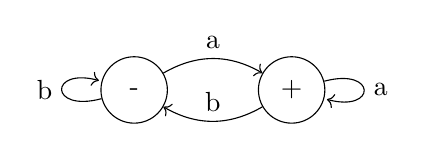
\begin{tikzpicture}

\fanonterminalnode {-2,0}{-};
\fanonterminalnode {0,0}{+};

\faarctransition{-}{+}{a}{30}{150};
\faarctransition {+}{-}{b}{210}{330};
\faloopright {+}{a};
\faloopleft {-}{b}
\end{tikzpicture}
 \caption{FA for accepting $(a+b)^*a$.}
\end{subfigure}

\begin{subfigure}[b]{0.45\textwidth}
\centering
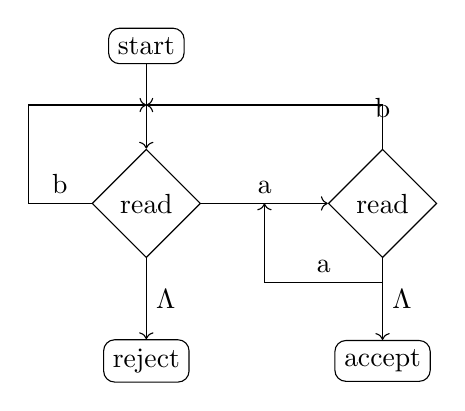
\begin{tikzpicture}

\pdaterminal {0,4}{start}{start}
\coordinate (start1) at (0, 3.25);
\pdaread {0,2}{nota}{read}
\coordinate (nota1) at (-1.5, 2);
\coordinate (nota2) at (-1.5, 3.25);
\pdaread {3,2}{reada}{read}
\coordinate (reada1) at (3, 3.25);
\coordinate (reada2) at (3, 1);
\coordinate (reada3) at (1.5, 1);
\coordinate (reada4) at (1.5, 2);
\pdaterminal {3,0}{accept}{accept}
\pdaterminal {0,0}{reject}{reject}
\pdatransition {start}{nota}{}
\pdatransition {nota}{reada}{a}
\pdarighttransition {nota}{reject}{$\Lambda$}
\pdarighttransition {reada}{accept}{$\Lambda$}
\pdaxthree {reada2}{reada3}{reada4}{a}
\pdaxthree {reada}{reada1}{start1}{b}
\pdaxfour {nota}{nota1}{nota2}{start1}{b}
\end{tikzpicture}
 \caption{PDA for accepting $(a+b)^*a$.}
\end{subfigure}

\caption{Both an FA and a PDA for accepting all strings that contain a double letter.}
\label{F.PDA.1}
\end{figure}
%----------------------------------------------------------

Figure~\ref{F.PDA.2} shows a PDA for accepting $a^nb^n$. Each time an $a$ is read, it is pushed onto the stack. Each time a $b$ is read, the stack is popped. If the stack is empty, the string is rejected because we had too many $b$'s. If we read an $a$ following a $b$, we also reject the string.

%----------------------------------------------------------
\begin{figure}[htbp]
\centering
\scalebox{.7}{
\begin{tikzpicture}

\pdaterminal {0,8}{start}{start}
\coordinate (start1) at (0, 7);
\pdapush {-2, 7}{pusha}{push a}
\pdaread {0,5}{reada}{read}
\coordinate (reada1) at (-2, 5);
\pdaread {0,2}{popa}{pop}
\coordinate (popa1) at (0, 4);
\pdaread {3, 2}{readb}{read}
\coordinate (readb1) at (3, 4);
\pdaread {6, 2}{popfinal}{pop}
\coordinate (popfinal1) at (6, 5);
\coordinate (popfinal2) at (9, 2);
\pdaterminal {0,-0.5}{reject1}{reject}
\pdaterminal {3,-0.5}{reject2}{reject}
\pdaterminal {6,-0.5}{accept}{accept}
\pdaterminal {9,-0.5}{reject3}{reject}

\pdatransition {start}{reada}{}
\pdalefttransition {reada}{popa}{b}
\pdarighttransition {popa}{reject1}{$\Lambda$}
\pdarighttransition {readb}{reject2}{a}
\pdarighttransition {popfinal}{accept}{$\Lambda$}
\pdatransition {pusha}{start1}{}
\pdatransition {popa}{readb}{a}
\pdatransition {readb}{popfinal}{$\Lambda$}
\pdaxthree {reada}{reada1}{pusha}{a}
\pdaxthree {readb}{readb1}{popa1}{b}
\pdaxthree {reada}{popfinal1}{popfinal}{$\Lambda$}
\pdaxthree {popfinal}{popfinal2}{reject3}{a}
\end{tikzpicture}
} % scale
\caption{PDA for accepting $a^nb^n$.}
\label{F.PDA.2}
\end{figure}
%----------------------------------------------------------

Since Figure~\ref{F.PDA.2} shows a solution to to $a^nb^n$, it is clear that PDAs are more powerful than FAs. Another example illustrates this. Figure~\ref{F.PDA.PAL.1} shows a PDA for accepting palindromes where the center letter is always an $x$. The reason for requiring the center $x$ is so the PDA knows when to transition from pushing input onto the stack to popping values off the stack.
%----------------------------------------------------------
\begin{figure}[htbp]
\centering
\scalebox{.7}{

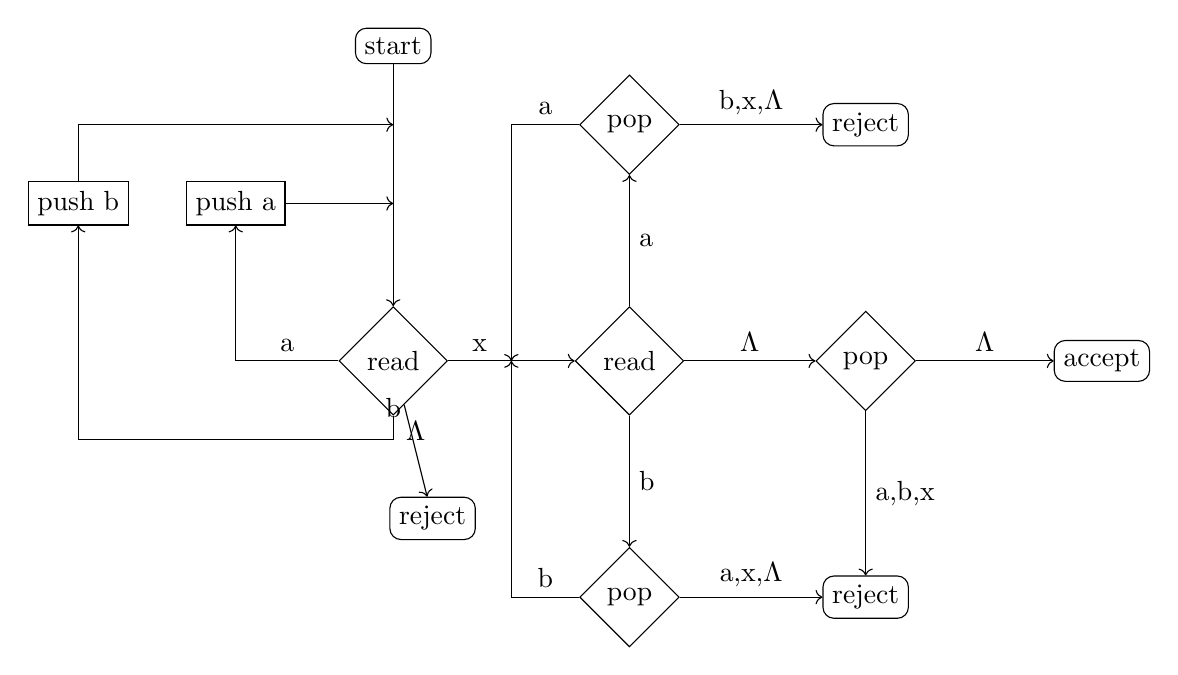
\begin{tikzpicture}

\pdaterminal {0,8}{start}{start}
\coordinate (start1) at (0, 7);
\coordinate (start2) at (0, 6);

\pdapush {-2, 6}{pusha}{push a}
\pdatransition {pusha}{start2}{}

\pdapush {-4, 6}{pushb}{push b}
\coordinate (pushb1) at (-4,7);
\pdaxthree {pushb}{pushb1}{start1}{}

\pdaread {0,4}{read1}{read}
\pdatransition {start}{read1}{}
\coordinate (read1b1) at (0, 3);
\coordinate (read1b2) at (-4, 3);
\coordinate (read1a) at (-2, 4);
\pdaxthree {read1}{read1a}{pusha}{a}
\pdaxfour {read1}{read1b1}{read1b2}{pushb}{b}


\pdaterminal {0.5,2}{reject1}{reject}
\pdatransition {read1}{reject1}{$\Lambda$}

\pdaread {3,4}{read2}{read}
\coordinate (read2a) at (1.5,4);
\pdaxthree {read1}{read2a}{read2}{x}

\pdaread {3,7}{popa}{pop}
\coordinate (popa1) at (1.5,7);
\pdarighttransition {read2}{popa}{a}
\pdaxthree {popa}{popa1}{read2a}{a}

\pdaread {3,1}{popb}{pop}
\coordinate (popb1) at (1.5,1);
\pdarighttransition {read2}{popb}{b}
\pdaxthree {popb}{popb1}{read2a}{b}

\pdaterminal {6,1}{reject2}{reject}
\pdatransition {popb}{reject2}{a,x,$\Lambda$}

\pdaterminal {6,7}{reject3}{reject}
\pdatransition {popa}{reject3}{b,x,$\Lambda$}

\pdaread {6,4}{popL}{pop}
\pdatransition {read2}{popL}{$\Lambda$}
\pdarighttransition {popL}{reject2}{a,b,x}

\pdaterminal {9,4}{accept}{accept}
\pdatransition {popL}{accept}{$\Lambda$}

\end{tikzpicture}
} % scale
\caption{PDA for accepting PALINDROME with a center $x$.}
\label{F.PDA.PAL.1}
\end{figure}
%----------------------------------------------------------

On the left part of the PDA, each time a value is read, it is pushed onto the stack. Once the center $x$ is read, each read requires a matching pop. If the value read doesn't match the value popped, the input is rejected. In order for the input to be accepted, the input and the stack have to become empty at the same time.

The purpose for requiring the center $x$ was to indicate when the PDA switches from pushing to popping. What if we wanted to have PALINDROME without the center-$x$ requirement? With FAs, we introduced non-determinism to make it easier to create an FA that matched a given regular express. What if we allowed non-determinism in PDAs? Figure~\ref{F.PDA.PAL.2} shows a PDA that accepts even-lengthed palindromes. It uses non-determinism to decide when to transition from pushing to popping. 
%----------------------------------------------------------
\begin{figure}[htbp]
\centering
\scalebox{.7}{

\begin{tikzpicture}

\pdaterminal {0,8}{start}{start}
\coordinate (start1) at (0, 7);
\coordinate (start2) at (0, 6);

\pdapush {-2, 6}{pusha}{push a}
\pdatransition {pusha}{start2}{}

\pdapush {-4, 6}{pushb}{push b}
\coordinate (pushb1) at (-4,7);
\pdaxthree {pushb}{pushb1}{start1}{}

\pdaread {0,4}{read1}{read}
\pdatransition {start}{read1}{}
\coordinate (read1b1) at (0, 3);
\coordinate (read1b2) at (-4, 3);
\coordinate (read1a) at (-2, 4);
\pdaxthree {read1}{read1a}{pusha}{a}
\pdaxfour {read1}{read1b1}{read1b2}{pushb}{b}

\pdaread {3,4}{read2}{read}
\coordinate (read2a) at (1.5,4);
\pdaxthree {read1}{read2a}{read2}{x}

\pdaread {3,7}{popa}{pop}
\coordinate (popa1) at (1.5,7);
\pdarighttransition {read2}{popa}{a}
\pdaxthree {popa}{popa1}{read2a}{a}
\pdatransition {read1}{popa}{a}

\pdaread {3,1}{popb}{pop}
\coordinate (popb1) at (1.5,1);
\pdarighttransition {read2}{popb}{b}
\pdaxthree {popb}{popb1}{read2a}{b}
\pdatransition {read1}{popb}{b}

\pdaread {6,4}{popL}{pop}
\pdatransition {read2}{popL}{$\Lambda$}

\pdaterminal {9,4}{accept}{accept}
\pdatransition {popL}{accept}{$\Lambda$}

\end{tikzpicture}
} % scale
\caption{PDA for accepting even-lengthed PALINDROMEs. Nondeterminism is used to transition from the first half of the palindrome to the second half.}
\label{F.PDA.PAL.2}
\end{figure}
%----------------------------------------------------------

In addition to including non-determinism, Figure~\ref{F.PDA.PAL.2} does not include reject states. Instead, if the PDA reaches a read or pop state without a transition on the symbol acquired, the machine crashes and the string is rejected. This is analogous to FAs that don't include dead states. 

With FAs we were able to show that DFAs and NFAs were equivalent. Anything you can do with one, you can do with the other. This is not true with PDAs. We will state without proof the non-deterministic PDAs are strictly more powerful than deterministic PDAs. Figure~\ref{F.machine.sizes.1} shows the relationship between the languages definable by the various machines we've encountered so far.
\begin{figure}[htbp]
\centering
\scalebox{.7}{
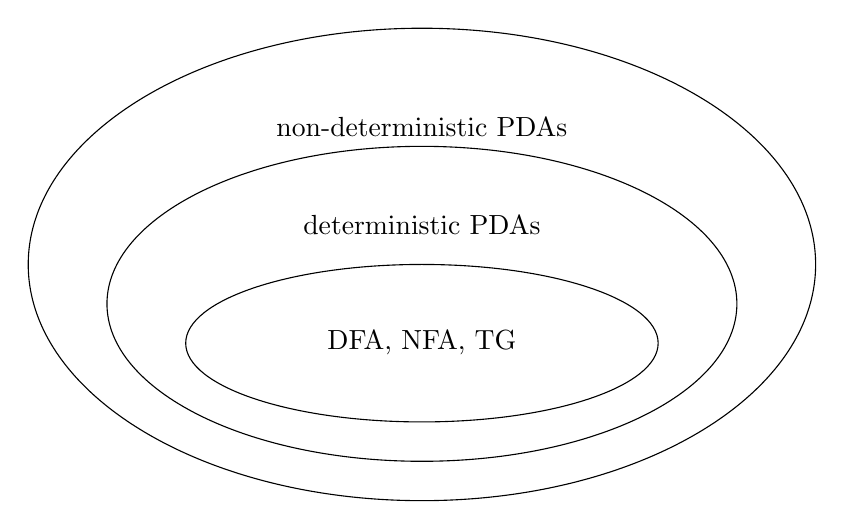
\begin{tikzpicture}
\draw (0,0) ellipse (3 and 1);
\draw (0,.5) ellipse (4 and 2);
\draw (0,1) ellipse (5 and 3);
\node at (0,0) {DFA, NFA, TG};
\node at (0,1.5) {deterministic PDAs};
\node at (0,2.75) {non-deterministic PDAs};
\end{tikzpicture}
} % scalebox
\caption{Relationship between the languages definable by the various machines we've encountered.}
\label{F.machine.sizes.1}
\end{figure}

\section {Conversion from CFG to PDA}
There is a form of PDA known as a ``central pop PDA'' that makes it easy to show a construction to go from any CFG to a PDA. A central pop PDA isn't a different type of machine, just a particular way of laying out a PDA. It is so named because there is a pop operation in the center of the diagram. Consider the PDA in Figure~\ref{F.PDA.CP.1}.
%----------------------------------------------------------
\begin{figure}[htbp]
\centering
\scalebox{.7}{

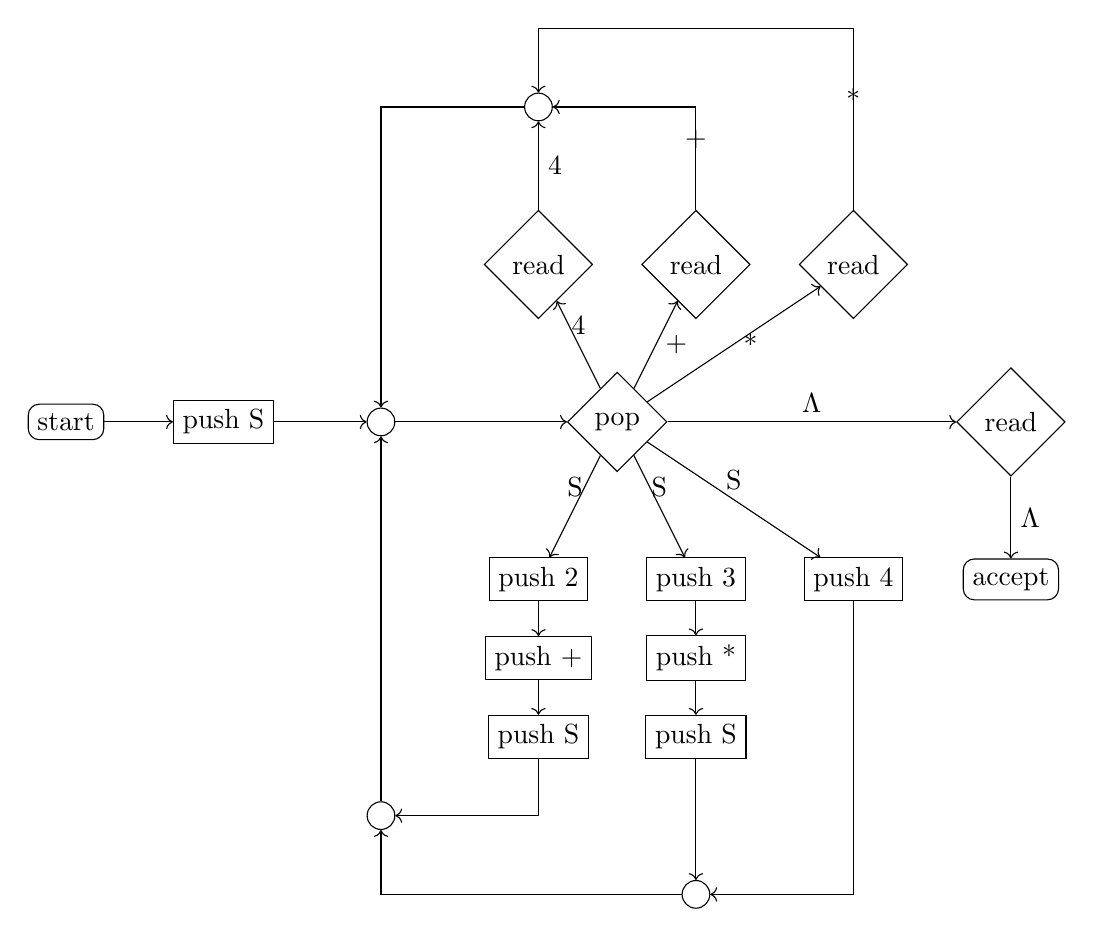
\begin{tikzpicture}

\pdaterminal {0,0}{start}{start}
\pdapush     {2,0}{pushS1}{push S}
\pdatransition {start}{pushS1}{}
\pdaconnect  {4,0} {pop1}
\pdatransition {pushS1}{pop1}{}
\pdaread     {7,0} {pop}{pop}
\pdatransition {pop1}{pop}{}

\pdapush     {6,-2}{push2}{push 2}
\pdatransition {pop}{push2}{S}
\pdapush     {6,-3}{push+}{push +}
\pdatransition {push2}{push+}{}
\pdapush     {6,-4}{pushS2}{push S}
\pdatransition {push+}{pushS2}{}
\coordinate (pushS2b) at (6, -5);
\pdaconnect {4, -5}{pop2}
\pdaxthree {pushS2}{pushS2b}{pop2}{}
\pdatransition {pop2}{pop1}{}

\pdapush     {8,-2}{push3}{push 3}
\pdatransition {pop}{push3}{S}
\pdapush     {8,-3}{push*}{push *}
\pdatransition {push3}{push*}{}
\pdapush     {8,-4}{pushS3}{push S}
\pdatransition {push*}{pushS3}{}
\pdaconnect {8, -6}{pop3}
\pdatransition {pushS3}{pop3}{}
\coordinate (pushS3b) at (4, -6);
\pdaxthree {pop3}{pushS3b}{pop2}{}

\pdapush     {10,-2}{push4}{push 4}
\pdatransition {pop}{push4}{S}
\coordinate (pushS4b) at (10, -6);
\pdaxthree {push4}{pushS4b}{pop3}{}

\pdaread {6, 2}{read4}{read}
\pdatransition {pop}{read4}{4}
\pdaread {8, 2}{read+}{read}
\pdarighttransition {pop}{read+}{+}
\pdaread {10, 2}{read*}{read}
\pdarighttransition {pop}{read*}{*}

\pdaconnect {6,4}{pop4}
\coordinate (pop1up) at (4, 4);
\coordinate (read+b) at (8, 4);
\coordinate (read*b) at (6, 5);
\coordinate (read*c) at (10, 5);

\pdarighttransition {read4}{pop4}{4}
\pdaxthree {read+}{read+b}{pop4}{+}
\pdaxfour {read*}{read*c}{read*b}{pop4}{*}
\pdaxthree {pop4}{pop1up}{pop1}{}

\pdaread {12, 0}{readL}{read}
\pdaterminal {12, -2}{accept}{accept}
\pdatransition {pop}{readL}{$\Lambda$}
\pdarighttransition {readL}{accept}{$\Lambda$}

\end{tikzpicture}
} % scale
\caption{PDA in central pop form or the CFG: $S \rightarrow S + 2\ |\ S * 3\ |\ 4$.}
\label{F.PDA.CP.1}
\end{figure}
%----------------------------------------------------------
The PDA starts by pushing the start symbol. The central pop then has one branch for each production as well as one branch for each terminal. If a non-terminal is popped off the stack, the right hand side of one of the productions for that non-terminal are pushed onto the stack from right to left. If a terminal is popped off the stack, then that terminal is read from the input. The central pop loop continues until the stack is empty. If the input is also empty, then the input is accepted as a word in the language.

Central pop PDAs have the property of producing top-down left-most derivations of the corresponding CFG. Since the right hand side of a production is pushed right to left, the top of the stack is either a terminal or the left-most non-terminal in the working string. The non-determinism in the PDA corresponds to the decision of which production to invoke in the derivation. Every valid left-most derivation is represented by a path through the PDA. Each time a terminal is encountered on the stack, the input is read to validate that the correct terminal is in the input stream. For this reason, only valid derivations are allowed. Since every valid left-most derivation is allowed and only valid derivations are allowed, the language represented by the central pop PDA exactly corresponds to the language represented by the corresponding CFG. Since a central pop PDA can be constructed for and CFG, this construction proves $L(CFG) \subseteq L(PDA)$

\section{Converting a PDA to a CFG}
There is another construction that allows us to convert any PDA into a CFG. In outline, there are steps to convert the PDA into a standard form. From that form, it is possible to construct a CFG that accepts the same language as the PDA. It would be analogous to showing a construction to convert an arbitrary FA into the form created by Thompson's Construction, and then showing how to go from that form into a regular expression.

Unfortunately, the conversion of the PDA into its standard form is complicated. The conversion from that to a CFG is even worse. Both are beyond the scope of A Very Simple Grammars Book, so they will not be included. However, the construction is sufficient to show that $L(PDA) \subseteq L(CFG)$. Since the previous section proved the reverse, we now have $L(CFG) = L(PDA)$.

\chapter{Theory of Context Free Languages}
In this chapter we will examine various properties of context free languages.
\section{All regular languages are context free}
When proving Kleene's Theorem, we used various constructions to show the equivalence of various forms of expressing a language. We will do the same here.

Take any FA, and give each state a unique name. To build an equivalent CFG, create a non-terminal for each state in the FA. For each edge in the FA, create a production as illustrated in Figure~\ref{F.FA.2.CFG}. For every final state in the FA, create a production with that state on the left-hand side and $\Lambda$ on the right.
%----------------------------------------------------------
\begin{figure}[hbt]
\centering
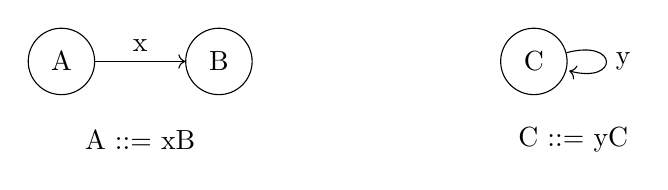
\begin{tikzpicture}

\fanonterminalnode {0,0}{A};
\fanonterminalnode {2,0}{B};
\fanonterminalnode {6,0}{C};

\fatransition{A}{B}{x};
\faloopright {C}{y};
\node at (1, -1) {A ::= xB};
\node at (6.5, -1) {C ::= yC};
\end{tikzpicture}
 \caption{Creating CFG productions from FA transitions.}
  \label{F.FA.2.CFG}
\end{figure}
%----------------------------------------------------------
For a complete example of using this construction, consider the FA in Figure~\ref{F.FA.to.CFG.example}. This FA is represented by the following CFG.
%----------------------------------------------------------
\begin{cfg}{}{}
Q\cfgprod{S}{aB}Q
Q\cfgprod{B}{bD}Q
Q\cfgprod{B}{aC}Q
Q\cfgprod{C}{aC}Q
Q\cfgprod{C}{$\Lambda$}Q
Q\cfgprod{D}{aB}Q
Q\cfgprod{D}{bE}Q
Q\cfgprod{E}{$\Lambda$}Q
\end{cfg}
%----------------------------------------------------------

%----------------------------------------------------------
\begin{figure}[hbt]
\centering
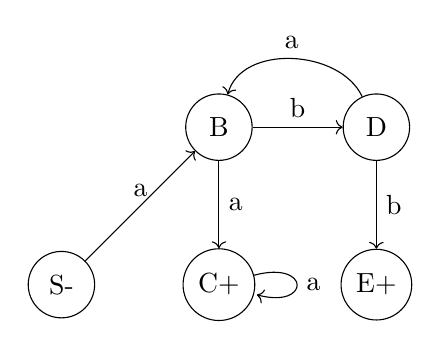
\begin{tikzpicture}

\fanonterminalnode {0,0}{S-};
\fanonterminalnode {2,2}{B};
\fanonterminalnode {2,0}{C+};
\fanonterminalnode {4,2}{D};
\fanonterminalnode {4,0}{E+};


\fatransition{S-}{B}{a};
\fatransition{B}{D}{b};
\farighttransition{B}{C+}{a};
\farighttransition{D}{E+}{b};
\faloopright {C+}{a};
\faarctransition {D}{B}{a}{115}{75};

\end{tikzpicture}
 \caption{Illustration of FA that is turned into a CFG.}
  \label{F.FA.to.CFG.example}
\end{figure}
%----------------------------------------------------------
\needswork
Need to do a proof that this works.

\section{Chompsky's Normal Form}
In this section we show that all grammars (for languages that don't include the empty string) can be transformed into Chompsky's Normal Form (CNF). In this form, all productions either have exactly two non-terminals on the right hand side (and no terminals) or exactly one terminal.

\subsection {Eliminating Lambda Productions}
CFG~\ref{C.with.lambda.1} shows a CFG that includes a $\Lambda$ production. CFG~\ref{C.no.lambda.1} shows an equivalent CFG without the $\Lambda$. There are two differences in the second CFG: the production for $L$ does not include the $\Lambda$ option, and there is a second production for $S$, which does not include the $L$. This additional production is necessary because in the original CFG, $L$ can be replaced with $\Lambda$ (nothing). Since that option was removed in the second CFG, we need an additional production that doesn't include $L$.
%----------------------------------------------------------
\begin{cfg}{CFG that includes a $\Lambda$ production.}{C.with.lambda.1}
Q\cfgprod{S}{STUFF L OTHER}Q
Q...Q
Q\cfgprod{L}{$\Lambda$ | a | b}Q
\end{cfg}
%----------------------------------------------------------
\begin{cfg}{Equivalent CFG without a $\Lambda$ production.}{C.no.lambda.1}
Q\cfgprod{S}{STUFF L OTHER}Q
Q\cfgprod{S}{STUFF OTHER}Q
Q...Q
Q\cfgprod{L}{a | b}Q
\end{cfg}
%----------------------------------------------------------

This transformation seems easy enough, but there is a potential problem. What if removing the $\Lambda$ from one production adds a $\Lambda$ to another. Consider the grammar in CFG~\ref{C.with.lambda.2}. If we follow the pattern from the previous example using this grammar, when we eliminate the $\Lambda$ from the $A$ production, we will introduce a $\Lambda$ to the $B$ production. When we eliminate that $\Lambda$, we will re-introduce the $\Lambda$ to the $A$ production.
%----------------------------------------------------------
\begin{cfg}{CFG that includes recursive $\Lambda$s.}{C.with.lambda.2}
Q\cfgprod{S}{STUFF}Q
Q...Q
Q\cfgprod{A}{$\Lambda$ | B}Q
Q\cfgprod{B}{STUFF | A}Q
\end{cfg}
%----------------------------------------------------------

The solution to recursive $\Lambda$s is to eliminate them all at once. The first step is to find all non-terminals that are nullable. That is, all non-terminals that can be replaced by a $\Lambda$ either directly or indirectly. A non-terminal is nullible if either:
\begin{quote}
{\ttfamily X} $\rightarrow \Lambda$\\
or\\
{\ttfamily X} $\rightarrow$ ... $\rightarrow \Lambda$\\
\end{quote}

We can find all the nullables using the following procedure:
\begin{enumerate}
\item Mark all non-terminals with $\Lambda$ productions.
\item If a production has only marked non-terminals on the right hand side, mark the non-terminal on the left hand side.
\item If Step~2 resulted in marking a new non-terminal, mark that non-terminal throughout the grammar.
\item Repeat steps 2 and 3 until no new non-terminals are marked.
\end{enumerate}
All terminals marked as a result of this procedure are nullable. Consider the following grammar (which happens to be for the language $(A+b)^*bb(a+b)^*$):
\begin{quote}
{\ttfamily S} $\rightarrow$ {\ttfamily X Y}\\
{\ttfamily X} $\rightarrow$ {\ttfamily Z b}\\
{\ttfamily Y} $\rightarrow$ {\ttfamily b W}\\
{\ttfamily Z} $\rightarrow$ {\ttfamily A B}\\
{\ttfamily W} $\rightarrow$ {\ttfamily Z}\\
{\ttfamily A} $\rightarrow$ {\ttfamily a A | b A | $\Lambda$}\\
{\ttfamily B} $\rightarrow$ {\ttfamily B a | B b | $\Lambda$}\\
\end{quote}
The productions for both $A$ and $B$ include $\Lambda$, so cross out every occurrence of $A$ and $B$. This results in the following grammar:
\begin{quote}
{\ttfamily S} $\rightarrow$ {\ttfamily X Y}\\
{\ttfamily X} $\rightarrow$ {\ttfamily Z b}\\
{\ttfamily Y} $\rightarrow$ {\ttfamily b W}\\
{\ttfamily Z} $\rightarrow$ {\ttfamily \sout{A} \sout{B}}\\
{\ttfamily W} $\rightarrow$ {\ttfamily Z}\\
{\ttfamily \sout{A}} $\rightarrow$ {\ttfamily a \sout{A} | b \sout{A} | $\Lambda$}\\
{\ttfamily \sout{B}} $\rightarrow$ {\ttfamily \sout{B} a | \sout{B} b | $\Lambda$}\\
\end{quote}
Since $Z$ has a production where everything on the right hand side is crossed out, cross out all occurrences of $Z$. This results in the following grammar:
\begin{quote}
{\ttfamily S} $\rightarrow$ {\ttfamily X Y}\\
{\ttfamily X} $\rightarrow$ {\ttfamily \sout{Z} b}\\
{\ttfamily Y} $\rightarrow$ {\ttfamily b W}\\
{\ttfamily \sout{Z}} $\rightarrow$ {\ttfamily \sout{A} \sout{B}}\\
{\ttfamily W} $\rightarrow$ {\ttfamily \sout{Z}}\\
{\ttfamily \sout{A}} $\rightarrow$ {\ttfamily a \sout{A} | b \sout{A} | $\Lambda$}\\
{\ttfamily \sout{B}} $\rightarrow$ {\ttfamily \sout{B} a | \sout{B} b | $\Lambda$}\\
\end{quote}
Since $W$ has a production where everything on the right hand side is crossed out, cross out all occurrences of $W$. This results in the following grammar:
\begin{quote}
{\ttfamily S} $\rightarrow$ {\ttfamily X Y}\\
{\ttfamily X} $\rightarrow$ {\ttfamily \sout{Z} b}\\
{\ttfamily Y} $\rightarrow$ {\ttfamily b \sout{W}}\\
{\ttfamily \sout{Z}} $\rightarrow$ {\ttfamily \sout{A} \sout{B}}\\
{\ttfamily \sout{W}} $\rightarrow$ {\ttfamily \sout{Z}}\\
{\ttfamily \sout{A}} $\rightarrow$ {\ttfamily a \sout{A} | b \sout{A} | $\Lambda$}\\
{\ttfamily \sout{B}} $\rightarrow$ {\ttfamily \sout{B} a | \sout{B} b | $\Lambda$}\\
\end{quote}
This didn't result in any additional non-terminals being crossed out, so we are done. The nullables are $A, B, W, Z$.

Now that we have a procedure for identifying all the nullables, we can give a procedure for eliminating $\Lambda$ productions. The procedure is as follows:
\begin{enumerate}
\item Identify all nullables.
\item Delete all $\Lambda$ productions.
\item For all productions with a nullable on the right hand side, create new productions for all subsets of the nullables, but don't introduce any new $\Lambda$ productions nor duplicates.
\end{enumerate}
To illustrate this procedure, consider the following CFG:
\begin{quote}
{\ttfamily S} $\rightarrow$ {\ttfamily a | X b Y | a Y a}\\
{\ttfamily X} $\rightarrow$ {\ttfamily Y | $\Lambda$}\\
{\ttfamily Y} $\rightarrow$ {\ttfamily b | X}\\
\end{quote}
The nullables are $X$ and $Y$. The second and third $S$ productions include nullables, so we need to create subsets. Take the production that has $X\ b\ Y$ on the right hand side. We will need new productions without the $X$, without the $Y$, and with neither. The production with $a\ Y\ a$ on the right hand side will need a new production without the $Y$. This yields the following CFG:
\begin{quote}
{1. \ttfamily S} $\rightarrow$ {\ttfamily a}\\
{2. \ttfamily S} $\rightarrow$ {\ttfamily X b Y | b Y | X b | b}\\
{3. \ttfamily S} $\rightarrow$ {\ttfamily a Y a | a a}\\
{4. \ttfamily X} $\rightarrow$ {\ttfamily Y}\\
{5. \ttfamily Y} $\rightarrow$ {\ttfamily b | X}\\
\end{quote}
Production 2 shows the second $S$ production and the new ones created from the subsets. Production~3 shows the third $S$ production and the new one created from the subsets. Productions 4 and 5 contain nullables, but a subset from those productions would create new $\Lambda$ productions, so no new productions are created from these.

Note that for Production~2, $b$ is not eliminated in the subset process because it is not nullable (as terminals never are).

\subsection{Eliminating Unit Productions}
A unit production is a production with just a single non-terminal on the right hand side. Note: It must be a single non-terminal. A production with a single terminal is not considered a unit production.

This procedure is similar the the procedure for eliminating $\Lambda$ productions, and like the $\Lambda$ procedure, we need to be aware of recursive unit productions. The procedure is as follows:
\begin{quote}
For every pair of terminals $A, B$ for which either:
\begin{quote}
{\ttfamily A} $\rightarrow$ {\ttfamily B}\\
{\ttfamily A} $\rightarrow$ {\ttfamily X$_1$} $\rightarrow$ {\ttfamily X$_2$} ... $\rightarrow$ {\ttfamily B}\\
\end{quote}
and the non-unit productions of $B$ 
\begin{quote}
{\ttfamily B} $\rightarrow\ S_1 | S_2 | S_3$
\end{quote}
create new productions for $A$:
\begin{quote}
{\ttfamily A} $\rightarrow S_1 | S_2 | S_3$\\
\end{quote}
Do all pairs simultaneously, and don't create any new unit productions.
\end{quote}

To identify all the unit pairs, start by making a list of all unit productions. Then invoke unit productions on the right hand side. Eliminate duplicates and any productions of the form {\ttfamily A} $\rightarrow$ {\ttfamily A}. Repeat this until no new unit pairs are identified.

This process is illustrated starting with the following CFG:
\begin{quote}
{1. \ttfamily S} $\rightarrow$ {\ttfamily EXPR}\\
{2. \ttfamily EXPR} $\rightarrow$ {\ttfamily EXPR + TERM}\\
{3. \ttfamily EXPR} $\rightarrow$ {\ttfamily TERM}\\
{4. \ttfamily TERM} $\rightarrow$ {\ttfamily TERM * num}\\
{5. \ttfamily TERM} $\rightarrow$ {\ttfamily num}\\
\end{quote}
Productions 1 and 3 are unit productions. Production~5 is not a unit production because even though the right hand side has only one symbol, it is a terminal, not a non-terminal. We can invoke production 3 on the right hand side of Production~1 yielding the following unit pairs:
\begin{quote}
{\ttfamily S} $\rightarrow$ {\ttfamily EXPR}\\
{\ttfamily S} $\rightarrow$ {\ttfamily TERM}\\
{\ttfamily EXPR} $\rightarrow$ {\ttfamily TERM}\\
\end{quote}
The non-unit productions are:
\begin{quote}
{\ttfamily EXPR} $\rightarrow$ {\ttfamily EXPR + TERM}\\
{\ttfamily TERM} $\rightarrow$ {\ttfamily TERM * num}\\
{\ttfamily TERM} $\rightarrow$ {\ttfamily num}\\
\end{quote}
Creating the new productions yields the following CFG:
\begin{quote}
{1. \ttfamily S} $\rightarrow$ {\ttfamily EXPR + TERM}\\
{2. \ttfamily S} $\rightarrow$ {\ttfamily TERM * num}\\
{3. \ttfamily S} $\rightarrow$ {\ttfamily num}\\
{4. \ttfamily EXPR} $\rightarrow$ {\ttfamily EXPR + TERM}\\
{5. \ttfamily EXPR} $\rightarrow$ {\ttfamily TERM * num}\\
{6. \ttfamily EXPR} $\rightarrow$ {\ttfamily num}\\
{7. \ttfamily TERM} $\rightarrow$ {\ttfamily TERM * num}\\
{8. \ttfamily TERM} $\rightarrow$ {\ttfamily num}\\
\end{quote}

\subsection{Eliminating mixed productions}
A mixed production is one that includes both terminals and non-terminals on the right hand side. To eliminate all mixed productions, create new non-terminals for each terminal then in each mixed production, replace the terminal with the corresponding non-terminal. 

Starting with the CFG we had at the end of the previous section, we need new terminals for $+\ *\ num$. These are as follows:
\begin{quote}
{\ttfamily PLUS} $\rightarrow$ {\ttfamily +}\\
{\ttfamily TIMES} $\rightarrow$ {\ttfamily *}\\
{\ttfamily NUM} $\rightarrow$ {\ttfamily num}\\
\end{quote}
Substituting these into the previous grammar we get:
\begin{quote}
{1. \ttfamily S} $\rightarrow$ {\ttfamily EXPR PLUS TERM}\\
{2. \ttfamily S} $\rightarrow$ {\ttfamily TERM TIMES NUM}\\
{3. \ttfamily S} $\rightarrow$ {\ttfamily num}\\
{4. \ttfamily EXPR} $\rightarrow$ {\ttfamily EXPR PLUS TERM}\\
{5. \ttfamily EXPR} $\rightarrow$ {\ttfamily TERM TIMES NUM}\\
{6. \ttfamily EXPR} $\rightarrow$ {\ttfamily num}\\
{7. \ttfamily TERM} $\rightarrow$ {\ttfamily TERM TIMES NUM}\\
{8. \ttfamily TERM} $\rightarrow$ {\ttfamily num}\\
{9. \ttfamily PLUS} $\rightarrow$ {\ttfamily +}\\
{10. \ttfamily TIMES} $\rightarrow$ {\ttfamily *}\\
{11. \ttfamily NUM} $\rightarrow$ {\ttfamily num}\\
\end{quote}
Note that we did not perform the substitution in productions 3, 6, or 8 because they are not mixed. They contain only a terminal. If we had performed the substitution on these productions, we would have created new unit productions. We went through a bunch of trouble to eliminate them, so we don't want to create new ones.

\subsection{Conversion to Chompsky's Normal Form}
The final step in converting to Chompsky's Normal Form is to transform all productions with more than two non-terminals on the right hand side into productions with exactly two. Consider the following production:
\begin{quote}
{\ttfamily A} $\rightarrow$ {\ttfamily B C D E}\\
\end{quote}
We will take the first two non-terminals on the right hand side and create a new non-terminal to replace them. We'll then repeat this until we are left with just two non-terminals. The first two are $B\ C$, so we will create a new non-terminal $Z$ to replace them.
\begin{quote}
{\ttfamily A} $\rightarrow$ {\ttfamily Z D E}\\
{\ttfamily Z} $\rightarrow$ {\ttfamily B C}\\
\end{quote}
We will then replace $Z\ D$ as follows:
\begin{quote}
{\ttfamily A} $\rightarrow$ {\ttfamily Y E}\\
{\ttfamily Z} $\rightarrow$ {\ttfamily B C}\\
{\ttfamily Y} $\rightarrow$ {\ttfamily Z D}\\
\end{quote}

It might be tempting to try to optimize the process by finding the minimum number of new non-terminals, but there is no need for this optimization. Simply start with the first production with three or more non-terminals and create a new non-terminal for the first two on the right hand side. Continue this process until all productions have exactly two non-terminals or a single terminal.

Performing this substitution on the expression grammar we had in the previous section we get:
\begin{quote}
{1. \ttfamily S} $\rightarrow$ {\ttfamily EXPRPL TERM}\\
{2. \ttfamily S} $\rightarrow$ {\ttfamily TERMTI NUM}\\
{3. \ttfamily S} $\rightarrow$ {\ttfamily num}\\
{4. \ttfamily EXPR} $\rightarrow$ {\ttfamily EXPRPL TERM}\\
{5. \ttfamily EXPR} $\rightarrow$ {\ttfamily TERMTI NUM}\\
{6. \ttfamily EXPR} $\rightarrow$ {\ttfamily num}\\
{7. \ttfamily TERM} $\rightarrow$ {\ttfamily TERMTI NUM}\\
{8. \ttfamily TERM} $\rightarrow$ {\ttfamily num}\\
{9. \ttfamily PLUS} $\rightarrow$ {\ttfamily +}\\
{10. \ttfamily TIMES} $\rightarrow$ {\ttfamily *}\\
{11. \ttfamily NUM} $\rightarrow$ {\ttfamily num}\\
{12. \ttfamily EXPRPL} $\rightarrow$ {\ttfamily EXPR PLUS}\\
{13. \ttfamily TERMTI} $\rightarrow$ {\ttfamily TERM TIMES}\\
\end{quote}

\subsection{Why Chompsky's Normal Form?}
The obvious question is, ``Why would we convert a grammar to Chompsky's Normal Form?'' The grammar presented at the end of the last section seems much more cumbersome than the original grammar, so why do this? The answer is that in practice we don't. We simply needed to prove that it can be done. The reason why this is interesting is that a grammar in Chompsky's Normal Form (CNF) will always produce binary parse trees. Since they are binary trees, we can define a relationship between the length of an input and the minimum tree depth needed to generate a string of that length. This will be useful when we want to prove that a language isn't context free.

In the previous sections, we showed that any CFG (that didn't allow empty strings) could be converted to CNF. To eliminate the exception, we could simply add a production {\ttfamily S}~$\rightarrow \Lambda$ to our CNF grammar if the original language included the empty string. Adding this production does not violate the binary tree nature of derivations. As a result, when we reason about grammars in CNF, the logic can be applied to any context free language.

\section{The Pumping Lemma for CFGs}
All productions for a CFG in Chompsky's Normal Form are in one of two forms: Live productions have exactly two non-terminals on the right hand side. They are ``live'' because when invoking one of these productions, the parse tree can continue to grow down that branch. Terminal productions (it's tempting to call them ``dead'') have exactly one terminal on the right hand side. These are terminal productions because the growth of the parse tree on this branch terminates when one of these productions is invoked.

When thinking about the shape of parse trees for CNF grammars, several things can be said:
\begin{enumerate}
\item The trees are binary trees because all live productions have two children.
\item All of the terminals are in leaf nodes of the tree.
\item Each leaf node has exactly one terminal.
\end{enumerate}

For a binary tree with $N$ leaf nodes, the minimum depth of the tree is $log_2(N)+1$. If the tree isn't balanced, it might be deeper, but it must be at least this deep. Since parse trees for CNF grammars are binary trees, we can use this fact when reasoning about parse trees for CNF grammars.

Suppose we have a grammar in CNF with $P$ live productions. Further suppose we have an input that is longer than $2^P$. For this input, the depth of the tree must be greater than $P$, and since we only have $P$ live productions, at least one of them must have been repeated on some path from the root to a leaf.

Note: We aren't claiming that all paths are that long, only that at least one path is. Nor are we claiming that all productions get repeated, only that at least one of them is. 

Consider the parse tree shown in Figure~\ref{F.CFG.pump.1}. Notice that the production $M$ was repeated on the path from the root to $X_1$. If the length of the input is greater than $2^P$, then this is required to have happened for some production $M$ on some path from the root to some leaf.
\begin{figure}[htb]
\centering
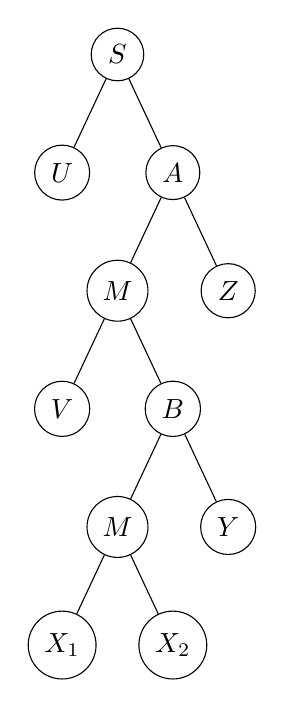
\begin{tikzpicture}[sibling distance=4em, 
  every node/.style = {shape=circle, draw, align=center}]
  \node {$S$}
      child { node {$U$} } 
		  child { node {$A$}
		    child {node {$M$}
				  child {node {$V$}}
					child {node {$B$}
					  child {node {$M$}
						  child {node {$X_1$}}
							child {node {$X_2$}}
						}
						child {node {$Y$}}
					}
			  }
			  child {node {$Z$}}
		};
\end{tikzpicture}
\caption[CNF Parse Tree]{A parse tree representing the derivation of some string based on a grammar in CNF. The nodes are labeled based on the production that was invoked to produce the children.}
\label{F.CFG.pump.1}
\end{figure}

Since both occurences of $M$ in this derivation use the same production, anything we can derive from the upper $M$, could also be derived from the lower $M$. Graphically, this would involve selecting the subtree based at the upper $M$ and pasting that subtree in the place of the lower $M$. Figure~\ref{F.CFG.pump.2} shows the result of this operation.
\begin{figure}[htb]
\centering
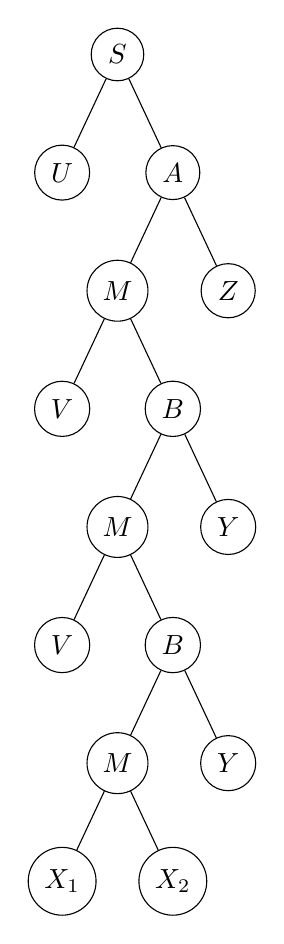
\begin{tikzpicture}[sibling distance=4em, 
  every node/.style = {shape=circle, draw, align=center}]
  \node {$S$}
      child { node {$U$} } 
		  child { node {$A$}
		    child {node {$M$}
				  child {node {$V$}}
					child {node {$B$}
		        child {node {$M$}
				      child {node {$V$}}
					    child {node {$B$}
					      child {node {$M$}
						      child {node {$X_1$}}
							    child {node {$X_2$}}
						    }
						    child {node {$Y$}}
					    }
			      }
						child {node {$Y$}}
					}
			  }
			  child {node {$Z$}}
		};
\end{tikzpicture}
\caption[CNF Parse Tree]{A parse tree when the subtree based at the upper $M$ from Figure~\ref{F.CFG.pump.1} is replicated at the lower $M$.}
\label{F.CFG.pump.2}
\end{figure}

Starting with the tree represented in Figure~\ref{F.CFG.pump.1}, if $u$ represents all terminals derived from the subtree based at $U$, and $v$ represents all the terminals derived from the subtree based at $V$, $x$ represents all the terminals derived from the subtrees based at $X_1$ and $X_2$, then likewise for $Y$ and $Z$, then the string represented by this tree is $uvxyz$. If we do the same substitutions for the tree in Figure~\ref{F.CFG.pump.2}, then the resulting string is $uv^2xy^2z$. If we do the copy and paste one more time, we will get $uv^3xy^3z$. We can continue to copy and paste to generate all strings $uv^nxy^nz$. This leads to the pumping lemma for context free languages.

\begin{lemma}
\label{T.CFL.pumping.lemma}
If $G$ is any CFG in CNF with $P$ live productions and $w$ is a word derived from $G$ with length greater than $2^P$, then we can divide $w$ into five substrings $w=uvxyz$, where $x$ is not the empty string and where both $v$ and $y$ are not the empty strings, such that all strings $uv^nxy^nz$ can also be generated by $G$.
\end{lemma}

The pumping lemma for context free languages bears some similarity to the pumping lemma for regular languages: Given a word of sufficient length, it can be broken into pieces such that all words derived as some function of those pieces are also in the language. The number of pieces is different, and the function is different, but the general form is the same. And like the pumping lemma for regular languages, the pumping lemma for context free languages can be used to prove a language is NOT context free, but it cannot be used to prove a language IS context free.

Consider the language $a^nb^nc^n$. Can we find assignments to $u,v,x,y,z$ such that all words of the form $uv^nxy^nz$ are in this language? Let's consider the possibilities:
\begin{enumerate}
\item If $v$ only has one type of letter (only $a$'s or only $b$'s or only $c$'s) and $y$ contains only that same letter (or is empty), then each time we pump the number of that letter will increase, but the number of the other letters will not change thus generating words not in the language.
\item If $v$ only has one type of letter and $v$ contains only a different letter, then each time we pump the number of two letters will increase, but the number of the other letter not change thus generating words not in the language.
\item If either $v$ or $y$ are strings containing different letters (for example, both $a$'s and $b$'s), then each time we pump we will generate extra transitions from one letter to another and thus strings not in the language.
\end{enumerate}
Since there is no way to assign $u,v,x,y,z$, such that all strings $uv^nxy^nz$ are in the language, $a^nb^nc^n$ must not be context free.

Consider the language $a^nb^ma^nb^m$. If we do the assignment where $u=\Lambda$, $v$ is the first group of $a$'s, $x$ is the first group of $b$'s, $y$ is the second group of $a$'s and $z$ is the second group of $b$'s, then all words $uv^nxy^nz$ are in the language. It turns out that this language is not context free, so we need a different approach to prove this.

There is a corollary to the pumping lemma that says that the length of the string $vxy$ must be less than $2^P$. To justify this corrollary, consider the parse tree given in Figure~\ref{F.CFG.pump.1}. The string $vxy$ is all the terminals generated by the subtree based at the upper $M$. By copying and pasting this subtree, we can generate any arbitrary length string. If we then took the upper most $M$ from the resulting tree and copied that, pasting it onto the lower most $M$, the resulting $vxy$ could be arbitrarily large. However, if we chose two $M$s that are closer to each other, the length of $vxy$ gets smaller. What the corrollary makes us do is choose two $M$s that are ``close'' rather than allowing us to choose two that are far apart.

Applying this corollary to the language $a^nb^ma^nb^m$, since we can choose any word with length greater than $2^P$, we will choose a word such that both $n$ and $m$ are greater than $2^P$. In this case, the assignment we chose above doesn't work. If $v$ consists of just the last $a$ in the first group and $y$ consists of just the first $a$ in the second group, while it is true that all $uv^nxy^nz$ are in the language, it is also true that the length of $uxy$ is greater than $2^P$ because it includes all $b$'s in the first group. Any assignment such that the length of $uxy$ is less than $2^P$ will generate words not in the language because this limitation prevents us from assigning $v$ to the first group of a letter and $y$ to the second group of that letter, and these are the only assignments that only generate words in the language. Therefore $a^nb^ma^nb^m$ is not context free.

\section {Properties of Context Free Languages}
\subsection {Context Free Languages are closed under union}
\begin{theorem}
\label{TH.CLF.union}
If $L_1$ and $L_2$ are two context free languages, then so is $L_1 \cup L_2$.
\end{theorem}
This can be proven using CFG's. If a subscript is added to all the non-terminals of the CFG for $L_1$ and a different subscript is added to all the non-terminals of the CFG for $L_2$, then a new CFG can be formed with a new start symbol as follows:
\begin{quote}
$S \rightarrow S_1\ |\ S_2$
\end{quote}
This can also be proven with PDA's using the same mechanism: create a new start state and have it transition to whereever the state states of the two PDA's transition to.

\subsection {Context Free Languages are closed under concatenation}
\begin{theorem}
\label{TH.CLF.concat}
If $L_1$ and $L_2$ are two context free languages, then so is $L_1 L_2$.
\end{theorem}
This can be proven using CFG's similar to the proof for union. The resulting CFG is:
\begin{quote}
$S \rightarrow S_1 S_2$
\end{quote}
However, proving by PDA is not so straight forward because the PDA for $L_1$ may require reading to the end of the input. This would not leave any input to fulfill the $L_2$ part of the word. However, the proof by CFG is sufficient to show that there is a PDA that accepts $L_1 L_2$.

\subsection {Context Free Languages are not closed under intersection}
First we must state that some context free languages are closed under intersection. In particular, all regular languages are also context free, and regular languages are closed under intersection. However, not all context free languages, when intersected, produce another context free languages. 

Consider the languages $L_1 = a^nb^na^m$ and $L_2 = a^nb^ma^n$. $L_1$ requires the first two groups of letters to be the same length. $L_2$ requires the first and third groups to be the same length. In order for a word to be in both $L_1$ and $L_2$, the first and second groups must be the same lenght and the first and third must be the same length. In other words, all three groups must be the same length so that $L_3 = L_1 \cap L_2 = a^nb^na^n$, which has already been proven to be non-context free.

\subsection {Context Free Languages are not closed under complement}
We will prove this by contradiction:

Suppose $L_1$ and $L_2$ are context free and that context free languages are closed under compliment. That would imply:
\begin{quote}
$L_1'$ and $L_2'$ are context free (our assumption)\\
$L_1' \cup L_2'$ is context free (CFLs are closed under union)\\
$(L_1' \cup L_2')'$ is context free (our assumption)\\
$L_1 \cap L_2$ is context free (De Morgan's Law)
\end{quote}
But since we've already shown that CFL's are not closed under intersection, the following statement is not true (in the general case), so our assumption must be false and we must conclude that CFL's are not closed under complement.

\subsection {Decidability on Emptiness}
To decide if $\Lambda$ is the language, use the nullable procedure to determine if the start symbol is nullable. If so, $\Lambda$ is in the language, so the language is not empty.

If $\Lambda$ is not in the language, convert the CFG to CNF preserving the entire language. The use the following procedure:
\begin{enumerate}
\item for each non-terminal that has a production with only terminals on the right-hand side, keep that production and delete all the others for that non-terminal.
\item For all other productions with that non-terminal on the right-hand side, substitute the string of terminals for the non-terminal.
\item Repeat steps 1 and 2 until either S has only terminals on the right-hand side or no further substitutions are possible.
\end{enumerate}
If the procedure results in a production with S on the left-hand side and a string of terminals on the right-hand side, then that is a word in the language. If the procedure does not result in such a production, then there are no words in the language.

\subsection{Decidability on whether a particular non-terminal ever gets used in derivations}
A non-terminal is considered ``unproductive'' if it cannot be used in derivations. If the procedure from the previous section is run until no further substitutions are possible (instead of stopping once S has all terminals on the right-hand side), then any non-terminal that does not have all terminals on the right-hand side is unproductive. This is true because there is no way for that non-terminal to be turned into all terminals. Once it appears in a derivation, the derivation will recurse forever.

The second step in determining if a non-terminal can ever be used is to determine if there is a path from S to that non-terminal. The following procedure can be used to determine if non-terminal X can be used in a derivation:
\begin{enumerate}
\item Eliminate all non-productive non-terminals from the grammar. In other words, delete all productions where a non-productive non-terminal appears on either the left-hand side or the right-hand side.
\item Mark all occurences of X (on either side)
\item Mark all non-terminals where that non-terminal is the left-hand side and there are any marks on the right-hand side. Note: it is not necessary for everything on the right-hand side to be marked. What we are marking is all non-terminals that can unltimately result in an X.
\item Repeat Step 2 until either S is marked or no additional non-terminals can be marked.
\end{enumerate}
If S gets marked, that means there is a path from S to X using only productive non-terminals. Since only productive non-terminals are included in the grammar at this point, they can all be turned into terminals resulting in a word in the language that included X in its derivation.

\subsection{Decidability on whether L is infinite}
Procedure 1: Convert the CFG to CNF and enumerate all possible words of length $s^P+1$. If any of these words are in the language, then the language is infinite. This is because we can then use the pumping lemma to generate arbitrarily large words.

Procedure 2: If there is any self embedding, L is infinte. Self embedding means that there is a form of recursion that allows the sub-tree under some non-terminal X to include an X. The following procedure can be used to determine if a particular production X allows self-embedding.
\begin{enumerate}
\item Eliminate all useless non-terminals (those that are either non-productive because they can't be reduced to all terminals, or those that can't be derived from the start symbol)
\item Replace X on the left-hand side with $\chi$
\item Mark all X's on the right-hand side
\item Mark all non-terminals that have any marks on the right-hand side
\item Repeat Step 4 until either $\chi$ is marked or no further non-terminals can be marked.
\end{enumerate}
If $\chi$ is marked, then X allows self-embedding and the language is infinte. If this procedure is repeated for all non-terminals until one is found that allows self-embedding, and no such non-terminal is found, then the language is finite.

\subsection {Decidability on whether a particular word is in a language}
For a non-deterministic approach, follow all possible paths through the PDA for that particular word. If any of them arrive at an accept state, then the word is accepted in the language.

For a deterministic approach, we need a deterministic derivation generator. These are known as parsers and they are the subject of books on compilers. We'll save this for later.

\subsection {Undecidable properties of Context Free Languages}
The following are undecidable:
\begin{enumerate}
\item Does $CFL_1 = CFL_2$?
\item Is a CFG ambiguous?
\item Given and ambiguous CFG, is there another non-ambiguous CFG that defines the same language?
\item Is the complement of a particular CFL context free?
\item Is the intersection of two CFL's context free?
\item Give two CFL's, do they have any words in common?
\item Are there any words NOT in a CFL? (Is the language $(a+b)^*$?)
\end{enumerate}

While context free languages are more powerful than regular languages, they also have fewer closure properties, and there is less we can decide about them. Despite the added power of context free languages, they aren't powerful enough to describe algorithms. For that we need a new class of languages, which will be discussed in the next part of this book.

\part{Beyond Context Free Languages}
\label{C.Beyond.Context.Free}
We saw that context free grammars could make use of a PDA's stack to define languages such as $a^nb^n$ that could not be defined with regular expressions. But the memory was limited: it consisted of a single stack. This limitation meant that context free grammars could not define a language such as $a^nb^nc^n$ because the stack could keep track of one set of letters, but not the next. It might be tempting to add another stack to keep track of a second group of letters, but what if we had more groups? We don't want a band-aid solution to solve a slightly more complex problem, we want a general solution for defining algorithms\footnote{It turns out that a second stack IS a general solution, but we'll get to that later.}. Alan Turing proposed a general purpose compute machine, and that machine forms the bases for general computability.

\chapter{Turing Machines}
When we introduced push down automata, we introduced the concept of a ``tape'' that contained the input and another tape that was used for the stack. Turing machines also make use of a read-write tape, but it is not limited to stack behavior. A Turing machine consists of the following:
\begin{itemize}
\item An infinite read-write tape that starts with the input and has $\Delta$ characters in all cells that don't have input characters.
\item A finite number of states that define behavior. Each state (instruction) performs the following:
\begin{enumerate}
\item Reads the tape
\item Writes the tape
\item Moves the tape one space either forward or backwards
\item Branches to the next instruction (state) based on the character read
\end{enumerate}
\end{itemize}
Figure~\ref{F.TM.1} shows a Turing Machine.
\begin{figure}[htbp]
\centering
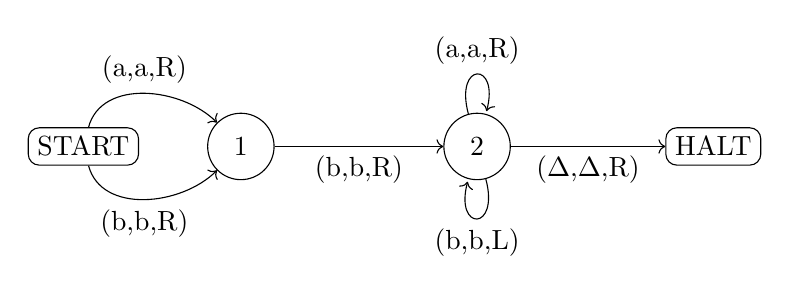
\begin{tikzpicture}
\pdaterminal{0,0}{START}{START}
\fanonterminalnode {2, 0}{1}
\fanonterminalnode {5, 0}{2}
\pdaterminal{8,0}{HALT}{HALT}
\faarctransition {START}{1}{(a,a,R)}{75}{135};
\faarcbelowtransition {START}{1}{(b,b,R)}{285}{225};
\falooptop{2}{(a,a,R)}
\faloopbottom{2}{(b,b,L)}
\fabelowtransition {1}{2}{(b,b,R)}
\fabelowtransition {2}{HALT}{($\Delta$,$\Delta$,R)}
\end{tikzpicture}
\caption[Sample Turing Machine]{Sample Turing Machine. The labels on the transitions are in the following form: (read, write, movement direction). The movement direction specifies the movement of the tape head, not the tape, so that ``R'' means the cell to the right of the current cell is the next cell that will be read. The input is accepted if the machine makes it to the HALT state.}
\label{F.TM.1}
\end{figure}
If this Turing Machine was given an input tape with ``$a,b,a,\Delta$'', the first $a$ would write the $a$ back to the tape, move the read/write head over the $b$, and transition to State~1. The $b$ would write the $b$ back to the tape, move the read/write head to the second $a$ and move to State~2. The next $a$ would leave us in State~2, and when we read the $\Delta$, we would reach the HALT state and accept the input.

If the input tape had ``$a,a,a,\Delta$'', then once we reached State~1 and read the second $a$, the machine would crash because there are no out-bound transitions on $a$.

If the input tape had ``$a,b,b,\Delta$'', when we reached State~2 and read the 2nd $b$, we would stay in State~2, but move the tape back to the first $b$. The next operation would leave us in State~2 and move the tape back to the $a$. The $a$ would move the tape to the first $b$, and then we would loop forever switching between the $a$ and the first $b$.

These three inputs, and their resulting behaviors, illustrate the three possibilities with Turing Machines:
\begin{enumerate}
\item Reach a HALT state and accept the input
\item Crash and reject the input
\item Loop forever and never make a decision
\end{enumerate}
Turing Machines can be represented in table form (much like transition tables for DFA's). Figure~\ref{F.TM.2} show such a table.
%----------------------------------------------------------
\begin{figure}[hbt]
\centering
\begin{tabular}{|c|c|c|c|c|}
\hline
State & Read & Write & Move & Next \\
\hline
1 & a & A & Right & 2 \\
\hline
2 & a & a & Right & 2 \\
\hline
2 & B & B & Right & 2 \\
\hline
2 & b & B & Left & 3 \\
\hline
3 & B & B & Left & 3 \\
\hline
3 & a & a & Left & 4 \\
\hline
3 & A & A & Right & 5 \\
\hline
4 & a & a & Left & 4 \\
\hline
4 & A & A & Right & 1 \\
\hline
5 & B & B & Right & 5 \\
\hline
5 & $\Delta$ & $\Delta$ & Right & HALT \\
\hline
\end{tabular}
\caption[Turing Machine Table]{This Turing Machine accepts the language $a^nb^n$.}
\label{F.TM.2}
\end{figure}
This machine accepts strings in the form $a^nb^n$. It does so by ``crossing out'' an $a$ and a matching $b$. The letters are crossed out by making them capital. State~1 crosses out the leftmost $a$. State~2 moves to the right looking for an un-crossed $b$. State~3 moves back to the left looking for an un-crossed $a$. If it finds one, State~4 looks for the right-most crossed $A$, which then goes back to State~1 to cross the next pair. If State~3 doesn't find an un-crossed $a$, it moves to State~5 looking for the end of tape. If there are too many $a$'s on the starting tape, the machine will crash in State~2 while looking for a uncrossed $b$ (it will reach the end of tape before finding an uncrossed $b$). If there are too many $b$'s on the tape, the machine will crash in State~5 while looking for the end of tape (it will find an uncrossed $b$ before getting to the end of tape).

We could extend this machine to handle languages such as $a^nb^nc^n$ by adding states to handle the $c$'s (doing so is left as a problem). This shows that Turing Machines can do things that CFG's can't. But we aren't just interested in being able to define more complex algorithms, we want to be able to do general computation.

\section{Computing with Turing Machines}
In order to do computation with TM's, we need a way to represent numbers on the input tape. We could, of course, use decimal notation, but that would create a proliferation of states because we'd need states for each digit. The simplest notation for numbers in TM's is unary. In unary, if we want to represent the number $N$, we simply list $N$ $a$'s. Suppose we wanted to add two numbers. The first number would consist of a string of $a$'s. The first number would be followed by a single $b$ to mark the boundary between numbers. The second number would consist of another string of $a$'s. How could we add these numbers? If we replace the $b$ with an $a$ and then delete the last $a$ on the tape, the tape would contain the result in unary. Figure~\ref{F.TM.add} shows such a TM.
%----------------------------------------------------------
\begin{figure}[hbt]
\centering
\begin{tabular}{|c|c|c|c|c|}
\hline
State & Read & Write & Move & Next \\
\hline
1 & a & a & Right & 1 \\
\hline
1 & b & a & Right & 2 \\
\hline
2 & a & a & Right & 2 \\
\hline
2 & $\Delta$ & $\Delta$ & Left & 3 \\
\hline
3 & a & $\Delta$ & Right & 3 \\
\hline
3 & $\Delta$ & $\Delta$ & Left & HALT \\
\hline
\end{tabular}
\caption[Turing Machine for adding]{This Turing Machine adds two numbers in unary.}
\label{F.TM.add}
\end{figure}
%----------------------------------------------------------

A similar approach could be used for performing subtraction. The last $a$ in the second number could be crossed out (replaced with $\Delta$), then a matching $a$ from the first number could be crossed out. This continues until there are no more $a$'s in the second group.

These two examples are hardly sufficient to argue that TM's are general purpose compute machines, but nevertheless, we will state (without proof) the following theorem:

\begin{theorem}
Everything that can be computed can be computed with a TM.
\end{theorem}

\chapter{Other Universal Compute Machines}
Turing Machines come in different forms based on the attributes of the tape. TM's can be constructed with tapes that are infinite in one direction, but the machine will crash if an attempt is made to move the tape before the beginning. It is also possible to construct a TM with a tape that is infinite in both directions. Both of these forms are equally powerful.

Another Universal Compute Machine is known as a Post Machine. These machines are just like PDA's except that instead of a stack, the ``push'' operation writes to the end of the tape. In other words, the tape is now a queue that is initialized with the input. There are proofs (by construction) that show that Post Machines and Turing Machines are equally powerful (either can be converted into the other).

Finally, there is a 2PDA: A PDA that has two stacks instead of one. Just like with Post Machines, there are proofs (by construction) that show that 2PDA's are equally powerful as Turing Machines.

\needswork Show constructions for TM=PM and TM=2PDA.

\chapter{Language Families}
We've already seen the following relationship between languages:
\begin{quote}
Regular Languages $\subset$ Deterministic Context Free Lanuages $\subset$ Non-deterministic Context Free Languages
\end{quote}
But we now have new families: those that can be defined by Turing Machines. How do these fit in this hierarchy?

\section {Context Sensitive Languages}
Context free languages are context free because, when building strings, anywhere a non-terminal appears it can be replaced using any production that has that non-terminal on the left-hand side. In other words, there is no context that says, ``You can replace A unless it is surrounded by $q$'s''. If we want to allow context, we can do so by relaxing the rules of what can go on the left hand side of a production. We can provide context by including more than just a non-terminal on the left-hand side. These grammars can take one of two forms. Consider the production:
\begin{quote}
$\alpha A \beta \rightarrow \alpha \gamma \beta$\\
where 
\begin{quote}
$A$ is a non-terminal and\\
$\alpha$, $\beta$, and $\gamma$ are strings of terminals and non-terminals such that $\gamma$ is not the empty string.
\end{quote}
\end{quote}
This production says that the non-terminal $A$ can be replaced with $\gamma$ provided that the $A$ is surrounded by the strings represented by $\alpha$ and $\beta$. Grammars in this form are known as context sensitive grammars. These languages can be recognized by Turing Machines where the tape length is bounded by some constant times the input length. The limit on the tape length really is a limit as we'll see in the next section.

\section{Recursive and Recursively Enumerable Languages}
The following production form is less restrictive than that for context sensitive languages:
\begin{quote}
$\alpha A \beta \rightarrow \gamma$\\
where 
\begin{quote}
$A$ is a non-terminal and\\
$\alpha$, $\beta$, and $\gamma$ are strings of terminals and non-terminals such that $\gamma$ is not the empty string.
\end{quote}
\end{quote}
The difference with this form is that the entire left-hand side is replaced, not just the non-terminal. This form of grammar leads to recursively enumerable languages. To explain this set of languages, let's first consider recursive languages.

Recall that Turing Machines can either halt, crash, or loop forever. If a TM can be constructed for a language such that all words in the language will cause the TM to halt and all words not in the language will cause the TM to crash, then this language is known as recursive. If a TM can be constructed which will halt on all words in the language, and will either crash or loop forever for words not in the language, then this languages is known as recursively enumerable. There are languages which are recursively enumerable, but not recursive. 

\subsection{The Halting Problem}
Suppose we defined a language as ``All programs that terminate''. We will restrict our programs to those that do not do any input so we don't have to worry about the input affecting whether or not the program terminates. To decide if a specific program was in the language, we could write a script that runs the program and if it terminates, prints the message ``This program is in the language.'' If we gave it a program in the language, we would get an answer. If we gave it a program not in the language (a program that loops forever), we would never get an answer. This is an example of the type of languages that are recursively enumerable, but not recursive.

Perhaps the script solution to the halting problem is a bad solution. Is there some other way to determine if a program loops forever? Let's assume it is possible. Let's assume we have an algorithm (meaning we can write a program to implement it) that returns \code{true} if a specified program halts and \code{false} if it doesn't. If so, we could write the following function:
\begin{quote}
\code{bool halts(program p);}
\end{quote}
We could then use that function in the following program:
\begin{lstlisting}[caption={Halting Problem program},label=L.halting]
program me
{
   while (halts(me))
	 {}
}
\end{lstlisting}
What does this program do? It passes itself into the \code{halt()} function. If the program \code{me} halts, then the \code{while} will loop forever, meaning \code{me} won't halt. But if \code{me} doesn't halt, then the \code{halts} function will return \code{false} so the \code{while} won't loop, and the program will terminate.

The result is that this program is self-contradicting. It is so because the \code{halts} function cannot, in fact, be written.

\section{Chompsky's Hierarchy}
Given our set of languages, we can now present Chompsky's Hierarchy. Each language category in the hierarchy is a strict subset of the languages higher in the hierarchy. The hierarchy is as follows (from smallest language to largest)
\begin{enumerate}
\item Regular Languages
\item Deterministic Context Free Languages
\item Non-Deterministic Context Free Languages
\item Context Sensitive Languages
\item Recursive Languages (not part of Chompsky's original hierarchy)
\item Recursively Enumerable Languages
\end{enumerate}
There is yet another category: Those that are not recursively enumerable. But before we introduce that category, we need to talk about Universal Turing Machines.

\section{Universal Turing Machines}
\label{S.universal.TM}
We have seen Turing Machines represented as diagrams, and we've seen them represented as tables. Is it possible to encode a Turing Machine onto a tape that can be used as the input to a Turing Machine? The answer is yes.

Let's restrict ourselves to Turing Machines over the alphabet $\Sigma = \{a\ b\}$. If we arrange the rows of the table form of a Turing Machine as follows:

\begin{tabular}{|c|c|c|c|c|}
\hline
State & Next & Read & Write & Move \\
\hline
$X_1$ & $X_2$ & $X_3$ & $X_4$ & $X_5$ \\
\hline
\end{tabular}

We can then encode each row as follows:
\begin{quote}
State: string of $X_1$ $a$'s followed by a $b$.\\
Next: string of $X_2$ $a$'s followed by a $b$.\\
Read, Write: 
\begin{quote}
$a$ is encoded as $aa$\\
$b$ is encoded as $ab$\\
\# is encoded as $ba$\\
$\Delta$ is encoded as $bb$
\end{quote}
Move: Left is encoded as $a$, and Right is encoded as $b$
\end{quote}
With this encoding, each row matches the regular expression $aa^*baa^*b(a+b)^5$. If we concatenate all rows together, it is always possible to determine where one row's encoding stops and the next row's encoding starts.

If we always use State~1 as the start state and State~2 as the HALT state, then we have a complete encoding suitable for any TM. What can we do with these encodings?

Recall that anything that can be computed can be computed by a TM. Clearly the behavior of a TM can be computed (we can build a machine - a TM - that can perform the calculation). So we should be able to create a TM that has as input:
\begin{quote}
\verb;<encoding of T>#<input word for T>;
\end{quote}
Where the behavior of the TM is as if T (encoded in the first part of the input) was run on the input (the second part of the input). This means that if T would halt on the input, the TM would also halt leaving the same characters on the tape. If T would crash, the TM would also crash. If T would loop forever, then the TM would also loop forever.

What have we just done? This TM is known as a Universal Turing Machine because it can emulate any TM (and is thus universal). It is a programmable computer. Instead of creating a new machine each time we want to solve a problem, we simply encode the problem on tape and feed it into our Universal TM.

This may not seem like a revolutionary thing to a modern reader (I assume you've been writing programs for a ``Universal'' machine prior to reading this), but it was revolutionary in its time. Not only is the Universal TM programmable, but it is even a Von Neumann machine: code and data are the same thing. 

Since Turing Machines are formal languages, and now also programmable machines, we can use the machine to answer questions about the languages that can be represented by TM's. This is, in part, how we know the Halting Problem cannot be solved. But we can go farther. We can now show that there are languages that are not recursively enumerable. 

\section{Non-Recursively Enumerable Languages}
The encoding discussed in Section~\ref{S.universal.TM} is called the Code Word Language (CWL). Using that encoding, we can now define the language ALAN:
\begin{quote}
ALAN = the set of all words in CWL that are NOT accepted by the TM's they represent or that do not represent TM's.
\end{quote}
In other words, ALAN can be thought of as either:
\begin{enumerate}
\item All programs that do not accept themselves as input.
\item All encodings \verb;<encoding of T>#<encoding of T>; where the Universal TM either crashes or loops.
\end{enumerate}
Let's consider some languages and figure out if the encoding for these languages are in ALAN.
\begin{quote}
L = \{all words with a double $a$\}
\end{quote}
Would the encoding for a machine that accepts all words with a double $a$ have a double $a$? Yes. The halt state is State~2 (which is encoded as a double $a$), and any machine that accepts any word must include the halt state, so the encoding would include a double $a$. Since the encoding would have a double $a$, the machine would accept itself, and so this word is not in ALAN.

What about \verb;L = {};? A TM that rejects all inputs would reject itself, so this word IS in ALAN.

What about PALINDROME? The CWL for PALINDROME almost certainly is not a palindrome, so this word is (most likely) in ALAN.

What about CWL = ``aabbab''. This is not a valid TM, so this is in ALAN.

But now we come to the interesting one. Is the CWL for a TM that accepts ALAN in ALAN? Let's assume ``yes''.

\begin{center}
\begin{tabular}{p{0.5\textwidth} l}
1) T accepts ALAN & 1) Definition of T\\
2) ALAN contains no cod word that is accepted by the machine it represents & 2) Definition of ALAN\\
3) CWL(T) is in ALAN & 3) Hypothesis\\
4) T accepts the word CWL(T) & 4) From 1 and 3\\
5) CWL(T) is not in ALAN & 5) From 2 and 4\\
6) Contradiction & 6) From 3 and 5
\end{tabular}
\end{center}

Since our assumption resulted in a contradiction, our assumption must be false. Let's try assuming the opposite: The CWL for a TM that accepts ALAN is not in ALAN.
\begin{center}
\begin{tabular}{p{0.5\textwidth} l}
1) T accepts ALAN & 1) Definition of T\\
2) If a word is not accepted by the machine it represents, it is in ALAN & 2) Definition of ALAN\\
3) CWL(T) is not in ALAN & 3) Hypothesis\\
4) T does not accept the word CWL(T) & 4) From 1 and 3\\
5) CWL(T) is in ALAN & 5) From 2 and 4\\
6) Contradiction & 6) From 3 and 5
\end{tabular}
\end{center}

What do we do now? Both the true and false assumptions resulted in contradictions. The problem is that there was another assumption we ignored. We assumed that there was a TM that accepts ALAN. It turns out that assumption was false. ALAN is not a recursively enumerable language, so there is no TM that accepts it. ALAN is not computable.

So now we have another category of language: those which are not computable. We will call this category ``Outer Space''. It includes language such as ALAN. I think poetry also fits this category (for a proof, read a few poems by ee cummings). We can't say much about languages in this category. We can't prove properties on this category because they are, by their very nature, not computable.

But there is one thing we can say about at least some of these languages. They come about if a language has the ability to be reflexive. That is, if the language can refer to itself. Consider the statement, 
\begin{quote}
This statement is a lie.
\end{quote}
This statement refers to itself (it is reflexive), and it uses that self-reference to be self-contradicting. The Halting Problem program did the same thing. Universal Turing Machines allow us to do the same thing. ALAN is example of a self-referential language, and it is this self-referentialness that makes in not computable.

Self referential statements are OK and interesting in the study of logic as a branch of philosophy. A philosophy class could spend hours of delight discussing whether ``This statement is a lie'' is true or not. However, these kinds of statements are anathema in mathematics. Mathematics used to be this pure scientific field where everything was either clearly true or clearly false (see \url{https://www.xkcd.com/435/}). Unfortunately, set theory is reflexive: you can have sets of sets. That's why set theory ``broke'' mathematics. Turing Machines are also reflexive. That's part of what makes computability (and programming in general) so interesting. 

\chapter{Conclusion}
Why study Computer Grammars (other than the fact that they're cool)? Some things that should be gained from this study:

You've learned about problem hardness in terms other that Big-O. Chompsky's Hierarchy describes language classes, but it also in some sense describes problem hardness. Consider the difference between a cellphone camera app that tags pictures taken in national parks vs. an app that tags pictures with birds in them (see \url{https://xkcd.com/1425/}). One problem is in the domain of regular languages. The other is probably at least recursive.

You've learned about problem transformations. For example, we can transform a regular expression problem into a DFA problem, which is much easier to write code for. In the field of software development, there are many transformations that can make writing software for a particular problem easier. If you can recognize such possible transformations, it will make it easier for you to solve problems.

You've learned new ways to express things. Some of your colleagues may not share the lingo, but if you know different ways to express things, you also know different ways to think about things. And this is really the point of this study: It should make you better at thinking about things than you used to be.

Returning to problem hardness, what problem domain (language category) would each of the following be in:
\begin{enumerate}
\item Design and build a steel girder bridge.
\item Design and build a power supply for a computer.
\item Design and build a compiler (or operating system or ...)
\end{enumerate}
I suspect the first two are in the domain of either regular or context free languages. There are known, almost turn-the-crank solutions to the first two. The third is at least context sensitive if not recursively enumerable. Some practitioners might argue that if we add the qualifier ``bug free'' to our compiler or operating system problem, that might put it in the outer space category.

A great deal of effort has been expended in trying to make software development resemble most other engineering disciplines, where many of the problems have known solutions (or at least procedures for finding solutions). Progress has been made, but software development is still a much fuzzier discipline. It remains, at least in part, an art not a science. I strongly suspect it will continue to be difficult to nail down (or engineer) because of the nature of the problems we are trying to solve. 

I hope this book has been valuable to you, and I hope you have gained at least some of the intended benefits of this study.

\begin{thebibliography}{9}
\bibitem {xkcd} \textsc{Munroe, Randal}: \textit{xkcd comics}, \url{xkcd.com}

\bibitem {comptheory} \textsc{Cohen, Daniel I.A.}: \textit{Introduction to Computer Theory}, John Wiley \& Sons, Inc., (1997).

\bibitem {FoundComp} \textsc{Carol Critchlow and David Eck}:\ \textit{Fundations of Computation}, \url{https://open.umn.edu/opentextbooks/textbooks/foundations-of-computation} (2011).
\end{thebibliography}

\end{document}
